\documentclass{article}

\usepackage{arxiv}

\usepackage[utf8]{inputenc} % allow utf-8 input
\usepackage[T1]{fontenc}    % use 8-bit T1 fonts
\usepackage{lmodern}        % https://github.com/rstudio/rticles/issues/343
\usepackage{hyperref}       % hyperlinks
\usepackage{url}            % simple URL typesetting
\usepackage{booktabs}       % professional-quality tables
\usepackage{amsfonts}       % blackboard math symbols
\usepackage{nicefrac}       % compact symbols for 1/2, etc.
\usepackage{microtype}      % microtypography
\usepackage{graphicx}

\title{Introducing ICBe: Very High Recall and Precision Event Extraction
from Narratives about International Crises}

\author{
    Rex W. Douglass
    \thanks{Correspondence should be addressed to Rex W. Douglass at
\href{mailto:rexdouglass@gmail.com}{\nolinkurl{rexdouglass@gmail.com}}.}
   \\
    University of California, San Diego \\
   \\
  \texttt{} \\
   \And
    Thomas Leo Scherer
   \\
    University of California, San Diego \\
   \\
  \texttt{} \\
   \And
    J. Andrés Gannon
   \\
    Vanderbilt University \\
   \\
  \texttt{} \\
   \And
    Erik Gartzke
   \\
    University of California, San Diego \\
   \\
  \texttt{} \\
   \And
    Jon Lindsay
   \\
    Georgia Institute of Technology \\
   \\
  \texttt{} \\
   \And
    Shannon Carcelli
   \\
    University of Maryland \\
   \\
  \texttt{} \\
   \And
    Jonathan Wilkenfeld
   \\
    University of Maryland \\
   \\
  \texttt{} \\
   \And
    David M. Quinn
   \\
    University of Maryland \\
   \\
  \texttt{} \\
   \And
    Catherine Aiken
   \\
    Georgetown University \\
   \\
  \texttt{} \\
   \And
    Jose Miguel Cabezas Navarro
   \\
    Universidad Mayor \\
   \\
  \texttt{} \\
   \And
    Neil Lund
   \\
    University of Maryland \\
   \\
  \texttt{} \\
   \And
    Egle Murauskaite
   \\
    University of Maryland \\
   \\
  \texttt{} \\
   \And
    Diana Partridge
   \\
    University of Maryland \\
   \\
  \texttt{} \\
  }


% tightlist command for lists without linebreak
\providecommand{\tightlist}{%
  \setlength{\itemsep}{0pt}\setlength{\parskip}{0pt}}


% Pandoc citation processing
\newlength{\cslhangindent}
\setlength{\cslhangindent}{1.5em}
\newlength{\csllabelwidth}
\setlength{\csllabelwidth}{3em}
\newlength{\cslentryspacingunit} % times entry-spacing
\setlength{\cslentryspacingunit}{\parskip}
% for Pandoc 2.8 to 2.10.1
\newenvironment{cslreferences}%
  {}%
  {\par}
% For Pandoc 2.11+
\newenvironment{CSLReferences}[2] % #1 hanging-ident, #2 entry spacing
 {% don't indent paragraphs
  \setlength{\parindent}{0pt}
  % turn on hanging indent if param 1 is 1
  \ifodd #1
  \let\oldpar\par
  \def\par{\hangindent=\cslhangindent\oldpar}
  \fi
  % set entry spacing
  \setlength{\parskip}{#2\cslentryspacingunit}
 }%
 {}
\usepackage{calc}
\newcommand{\CSLBlock}[1]{#1\hfill\break}
\newcommand{\CSLLeftMargin}[1]{\parbox[t]{\csllabelwidth}{#1}}
\newcommand{\CSLRightInline}[1]{\parbox[t]{\linewidth - \csllabelwidth}{#1}\break}
\newcommand{\CSLIndent}[1]{\hspace{\cslhangindent}#1}

\usepackage[utf8]{inputenc}
\usepackage{pifont}
\usepackage{newunicodechar}
\newunicodechar{✓}{\ding{51}}
\newunicodechar{✗}{\ding{55}}
\usepackage{array}
\usepackage{ctable}
\usepackage{booktabs}
\usepackage{longtable}
\usepackage{array}
\usepackage{multirow}
\usepackage{wrapfig}
\usepackage{colortbl}
\usepackage{pdflscape}
\usepackage{tabu}
\usepackage{threeparttable}
\usepackage{threeparttablex}
\usepackage[normalem]{ulem}
\usepackage{makecell}
\usepackage{titlesec}
\usepackage[parfill]{parskip}
\usepackage{makecell}
\usepackage{graphicx}
\usepackage{setspace}
\usepackage{cellspace}
\setlength\cellspacetoplimit{0.8ex}
\renewcommand{\arraystretch}{0.8}
\AtBeginEnvironment{lltable}{\singlespacing}
\usepackage{subcaption}
\usepackage{atbegshi}% http://ctan.org/pkg/atbegshi
\usepackage{float}
\usepackage[algo2e]{algorithm2e}
\usepackage{changepage}
\renewcommand{\bibliography}[1]{}
\usepackage{multirow}
\usepackage{multicol}
\usepackage{colortbl}
\usepackage{hhline}
\usepackage{longtable}
\usepackage{array}
\usepackage{hyperref}
\begin{document}
\maketitle


\begin{abstract}
How do international crises unfold? We conceptualize international
relations as a strategic chess game between adversaries and develop a
systematic way to measure pieces, moves, and gambits accurately and
consistently over a hundred years of history. We introduce a new
ontology and dataset of international events called ICBe based on a very
high-quality corpus of narratives from the International Crisis Behavior
(ICB) Project. We demonstrate that ICBe has higher coverage, recall, and
precision than existing state of the art datasets and conduct two
detailed case studies of the Cuban Missile Crisis (1962) and the
Crimea-Donbas Crisis (2014). We further introduce two new event
visualizations (event iconography and crisis maps), an automated
benchmark for measuring event recall using natural language processing
(synthetic narratives), and an ontology reconstruction task for
objectively measuring event precision. We make the data, supplementary
appendix, replication material, and visualizations of every historical
episode available at a companion website www.crisisevents.org.
\end{abstract}

\keywords{
    Diplomacy
   \and
    War
   \and
    Crises
   \and
    International Affairs
   \and
    Computational Social Science
  }

\hypertarget{introduction}{%
\section{Introduction}\label{introduction}}

If we could record every important interaction between countries in all
of diplomacy, military conflict, and international political economy,
how much unique information would this chronicle amount to, and how
surprised would we be to see something new? In other words, what is the
entropy of international relations? This record could in principle be
unbounded, but the central conceit of social science is that there are
structural regularities that limit what actors can do, their best
options, and even which actors are likely to survive (Brecher 1999;
Reiter 2015). If so, then these events can be systematically measured,
and accordingly, massive effort is expended in social science attempting
to record these regularities.\footnote{See work on crises (Brecher and
  Wilkenfeld 1982; Beardsley et al. 2020), militarized disputes (Palmer
  et al. 2021; Gibler 2018; Maoz et al. 2019), wars (Sarkees and Wayman
  2010; Reiter, Stam, and Horowitz 2016), organized violence (Ralph
  Sundberg and Mihai Croicu 2016; Pettersson and Eck 2018), political
  violence (Raleigh et al. 2010), sanctions (Felbermayr et al. 2020),
  trade (Barari and Kim, n.d.), and international agreements (Kinne
  2020; Owsiak, Cuttner, and Buck 2018; Vabulas and Snidal 2021),
  dispute resolution (Vabulas and Snidal 2021; Frederick, Hensel, and
  Macaulay 2017), and diplomacy (Moyer, Turner, and Meisel 2020; Sechser
  2011).} Thanks to improvements in natural language processing, more
open-ended efforts have begun to capture entire unstructured streams of
events from international news reports.\footnote{See Li et al. (2021);
  Halterman (2020); Brandt et al. (2018); Boschee et al. (2015); Hegre
  et al. (2020); Grant et al. (2017). On event extraction from images
  and social media see Zhang and Pan (2019) and Steinert-Threlkeld
  (2019).} How close these efforts are to accurately measuring all or
even most of what is essential in international relations is an open
empirical question, one for which we provide new evidence here.

Our contribution is a high coverage ontology and event dataset for key
historical episodes in 20th and 21st-century international relations. We
develop a large, flexible ontology of international events with the help
of both human coders and natural language processing. We apply it
sentence-by-sentence to an unusually high-quality corpus of historical
narratives of international crises (Brecher 1999; Brecher, James, and
Wilkenfeld 2000; Wilkenfeld and Brecher 2000; James 2019; Iakhnis and
James 2019). The result is a new lower bound estimate of how much
actually happens between states during pivotal historical episodes. We
then develop several methods for objectively gauging how well these
event codings reconstruct the information contained in the original
narrative. We conclude by benchmarking our event codings against several
current state of the art event data collection efforts. We find that
existing systems produce sequences of events that do not contain enough
information to reconstruct the underlying historical episode. The
underlying fine-grained variation in international affairs is
unrecognizable through the lens of current quantification efforts.

This is a measurement paper that makes the following argument --- there
is a real-world unobserved latent concept known as international
relations, we propose a method for systematically measuring it, we
successfully apply this method producing a new large-scale set of
measurements, and those measurements exhibit several desirable kinds of
internal and external validity, and those measurements out-perform other
existing approaches. The article organizes that argument into eight
sections: task definition; corpus; priors/existing state of the art;
ICBe coding process; internal consistency; case study selection; recall;
and precision. A final section concludes.

\hypertarget{task-definition}{%
\section{Task Definition}\label{task-definition}}

We consider the measurement task of absstracting discrete events about a
historical episode in international relations. The easiest way to convey
the task is with an example. Figure 1 shows a narrative account of the
Cuban Missile Crisis (1962) alongside a mapping from each natural
language sentence to discrete machine-readable abstractive events.
Formally, a historical episode, \(H\), is demarcated by a period of time
\([T_{start}, T_{end}] \in T\), a set of Players \(p \in P\), and a set
of behaviors they undertook during that time \(b \in B\). International
Relations, \(IR\), is the system of regularities that govern the
strategic interactions that world actors make during a historical
episode, given their available options, preferences, beliefs, and
expectations of choices made by others. We observe neither \(H\) nor
\(IR\) directly. Rather the Historical Record, \(HR\), produces
documents \(d \in D\) containing some relevant and true (as well as
irrelevant and untrue) information about behaviors that were undertaken
recorded in the form of unstructured natural language text. The task is
to combine informative priors about \(IR\) with an unstructured corpus
\(D\) to produce a series of structured discrete events, \(e \in E\),
that have high coverage, precision, and recall over what actually took
place in history, \(H\).

\clearpage

\begin{figure}[H]
\caption{Cuban Missile Crisis (1962) - ICB Narrative vs. ICBe Events \label{fig:case_study_cuban_precision}}
\centering{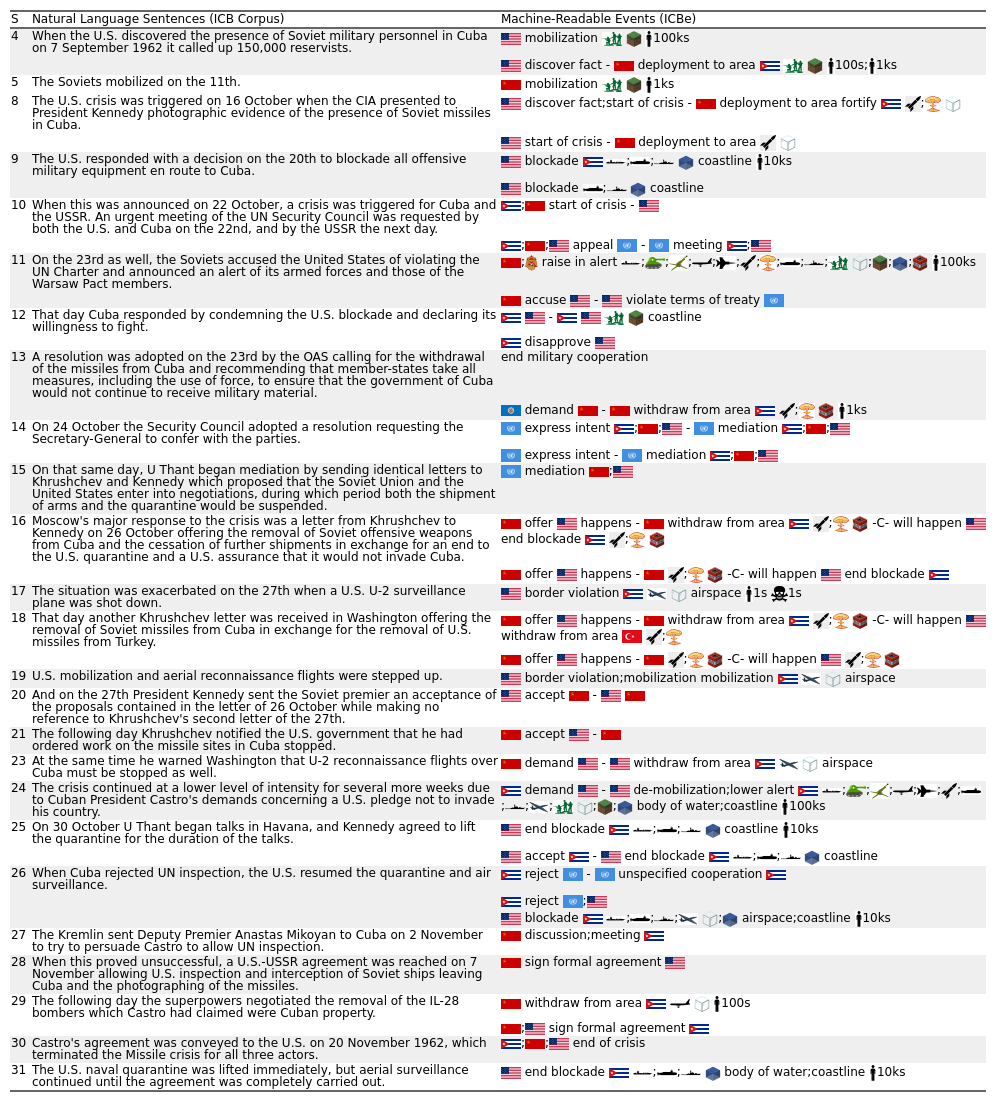
\includegraphics[height=19cm]{"./case_study_cuban_precision.png"}}
\end{figure}
\clearpage

\hypertarget{corpus}{%
\section{Corpus}\label{corpus}}

For our corpus, \(D\), we select a set of unusually high-quality
historical narratives from the International Crisis Behavior (ICB)
project (\(n=471\))(Supplementary Information (SI) Appendix 1.1)(Brecher
et al. 2017; Brecher and Wilkenfeld 1997). Their domain is 20th and
21st-century crises, defined as a change in the type, or an increase in
the intensity, of disruptive interaction with a heightened probability
of military hostilities that destabilizes states' relationships or
challenges the structure of the international system (Brecher and
Wilkenfeld 1982).\footnote{On near crises see Iakhnis and James (2019).}
Crises are a significant focus of detailed single case studies and case
comparisons because they provide an opportunity to examine behaviors in
IR short of, or at least prior to, full conflict (Holsti 1965; Paige
1968; Allison and Zelikow 1971; Snyder and Diesing 1977; Gavin 2014;
George and Smoke 1974; Brecher and Wilkenfeld 1982; Gaddis 1987; Brecher
and James 1988). Case selection was exhaustive based on a survey of
world news archives and region experts, cross-checked against other
databases of war and conflict, and non-English sources (Kang and Lin
2019; Brecher et al. 2017, 59). Each narrative was written by consensus
by a small number of scholars, using a uniform coding scheme, with
similar specificity (Hewitt 2001). The corpus is unique in IR because it
is designed to be used in a downstream quantitative coding project.

\hypertarget{prior-beliefs-about-ir-ontological-coverage-and-the-existing-state-of-the-art}{%
\section{Prior Beliefs about IR, Ontological Coverage, and the Existing
State of the
Art}\label{prior-beliefs-about-ir-ontological-coverage-and-the-existing-state-of-the-art}}

Next, we draw informative prior beliefs about the underlying process of
IR that we expect to govern behavior during historical episodes and
their conversion to the historical record. We organize our prior beliefs
along two overarching axes, summarized in detail by Table 1.

The first axis (rows) represents the types of information we expect to
find in IR and forms the basis for our proposed ontology. We employ a
metaphor of a chess game, with players (polities, rebel groups, IGOs,
etc.), pieces (military platforms, civilians, domains), and behaviors
(think, say, do). Precise sequencing is required to capture gambits
(sequences of moves) and outcomes (victory, defeat, peace, etc.), while
precise geo-coding is required to understand the chessboard (medium of
conflict). We find 472 actors and 117 different behaviors.\footnote{See
  the full codebook on Github Repository
  \href{https://urldefense.com/v3/__https://github.com/CenterForPeaceAndSecurityStudies/ICBEventData__;!!Mih3wA!WxDJtEczKfxGTh0S2Krunap8ReymFEL5iTWaSfOHeqlSdyfRx77zmjBSWO1OAm13$}{ICBEventData}.}

We base our informed priors primarily on two sources of information. The
first is the extensive existing measurement efforts of IR which we
provide citations alongside each concept. Second, we performed
preliminary natural language processing of the corpus and identified
named entities and behaviors mentioned in the text. Verbs were matched
to the most likely definition found in Wordnet (Miller 1995), tallied,
and then aggregated into a smaller number of hypernyms balancing
conceptual detail and manageable sparsity for human coding (SI Appendix
1.2).

The second axis (columns) compares the very high ontological coverage of
ICBe to existing state of the art systems in production and with global
coverage. They begin with our contribution ICBe, alongside other
event-level datasets including CAMEO dictionary lookup-based systems
(Historical Phoenix (Althaus et al. 2019); ICEWS (Boschee et al. 2015;
Hegre et al. 2020); Terrier (Grant et al. 2017)), the Militarized
Interstate Disputes Incidents dataset, and the UCDP-GED dataset (Ralph
Sundberg and Mihai Croicu 2016; Pettersson and Eck 2018; Sundberg and
Melander 2013).\footnote{Other related datasets that insufficiently
  overlap ICBe's domain for comparison include BCOW (Leng and Singer
  1988), WEIS (McClelland 1978), CREON (Hermann 1984), CASCON
  (Bloomfield and Moulton 1989), SHERFACS (Sherman 2000), Real-Time
  Phoenix (Brandt et al. 2018), and COfEE (Balali, Asadpour, and Jafari
  2021) (see histories in Merritt (1994) and Schrodt and Hall (2006)).}
The final set of columns compares episode-level datasets beginning with
the original ICB project (Brecher et al., n.d.; Brecher and Wilkenfeld
1982; Beardsley et al. 2020); the Militarized Interstate Disputes
dataset (Palmer et al. 2021; Gibler 2018; Braithwaite 2010, 2009), and
the Correlates of War (Sarkees and Wayman 2010). With the exception of
large-scale CAMEO dictionary-based systems, the existing state of the
art quantitative datasets ignore the vast majority of the information
content found in international relations.\footnote{See (Balali,
  Asadpour, and Jafari 2021) for a recent review of ontological depth
  and availability of Gold Standard example text.}

\clearpage

\providecommand{\docline}[3]{\noalign{\global\setlength{\arrayrulewidth}{#1}}\arrayrulecolor[HTML]{#2}\cline{#3}}

\setlength{\tabcolsep}{2pt}

\renewcommand*{\arraystretch}{0.75}

\begin{longtable}[c]{|p{0.10in}|p{2.00in}|p{1.60in}|p{0.22in}|p{0.22in}|p{0.22in}|p{0.22in}|p{0.22in}|p{0.22in}|p{0.22in}|p{0.22in}|p{0.22in}}

\caption{Ontological coverage of ICBe versus existing State of the Art
}\\

\hhline{>{\arrayrulecolor[HTML]{000000}\global\arrayrulewidth=2pt}->{\arrayrulecolor[HTML]{000000}\global\arrayrulewidth=2pt}->{\arrayrulecolor[HTML]{000000}\global\arrayrulewidth=2pt}->{\arrayrulecolor[HTML]{000000}\global\arrayrulewidth=2pt}->{\arrayrulecolor[HTML]{000000}\global\arrayrulewidth=2pt}->{\arrayrulecolor[HTML]{000000}\global\arrayrulewidth=2pt}->{\arrayrulecolor[HTML]{000000}\global\arrayrulewidth=2pt}->{\arrayrulecolor[HTML]{000000}\global\arrayrulewidth=2pt}->{\arrayrulecolor[HTML]{000000}\global\arrayrulewidth=2pt}->{\arrayrulecolor[HTML]{000000}\global\arrayrulewidth=2pt}->{\arrayrulecolor[HTML]{000000}\global\arrayrulewidth=2pt}->{\arrayrulecolor[HTML]{000000}\global\arrayrulewidth=2pt}-}

\multicolumn{1}{!{\color[HTML]{000000}\vrule width 2pt}>{\centering}p{\dimexpr 0.1in+0\tabcolsep+0\arrayrulewidth}}{\rotatebox[origin=c]{270}{\fontsize{6}{6}\selectfont{\textcolor[HTML]{000000}{}}}} & \multicolumn{1}{!{\color[HTML]{000000}\vrule width 0pt}>{\centering}p{\dimexpr 2in+0\tabcolsep+0\arrayrulewidth}}{\rotatebox[origin=c]{270}{\fontsize{6}{6}\selectfont{\textcolor[HTML]{000000}{Concept}}}} & \multicolumn{1}{!{\color[HTML]{000000}\vrule width 0pt}>{\centering}p{\dimexpr 1.6in+0\tabcolsep+0\arrayrulewidth}}{\rotatebox[origin=c]{270}{\fontsize{6}{6}\selectfont{\textcolor[HTML]{000000}{Literature}}}} & \multicolumn{1}{!{\color[HTML]{666666}\vrule width 1pt}>{\centering}p{\dimexpr 0.22in+0\tabcolsep+0\arrayrulewidth}}{\rotatebox[origin=c]{270}{\fontsize{6}{6}\selectfont{\textcolor[HTML]{000000}{ICBe}}}} & \multicolumn{1}{!{\color[HTML]{000000}\vrule width 0pt}>{\centering}p{\dimexpr 0.22in+0\tabcolsep+0\arrayrulewidth}}{\rotatebox[origin=c]{270}{\fontsize{6}{6}\selectfont{\textcolor[HTML]{000000}{Phoenix}}}} & \multicolumn{1}{!{\color[HTML]{000000}\vrule width 0pt}>{\centering}p{\dimexpr 0.22in+0\tabcolsep+0\arrayrulewidth}}{\rotatebox[origin=c]{270}{\fontsize{6}{6}\selectfont{\textcolor[HTML]{000000}{Terrier}}}} & \multicolumn{1}{!{\color[HTML]{000000}\vrule width 0pt}>{\centering}p{\dimexpr 0.22in+0\tabcolsep+0\arrayrulewidth}}{\rotatebox[origin=c]{270}{\fontsize{6}{6}\selectfont{\textcolor[HTML]{000000}{ICEWs}}}} & \multicolumn{1}{!{\color[HTML]{000000}\vrule width 0pt}>{\centering}p{\dimexpr 0.22in+0\tabcolsep+0\arrayrulewidth}}{\rotatebox[origin=c]{270}{\fontsize{6}{6}\selectfont{\textcolor[HTML]{000000}{MID\ Incidents}}}} & \multicolumn{1}{!{\color[HTML]{666666}\vrule width 1pt}>{\centering}p{\dimexpr 0.22in+0\tabcolsep+0\arrayrulewidth}}{\rotatebox[origin=c]{270}{\fontsize{6}{6}\selectfont{\textcolor[HTML]{000000}{UCDP-GED}}}} & \multicolumn{1}{!{\color[HTML]{000000}\vrule width 0pt}>{\centering}p{\dimexpr 0.22in+0\tabcolsep+0\arrayrulewidth}}{\rotatebox[origin=c]{270}{\fontsize{6}{6}\selectfont{\textcolor[HTML]{000000}{ICB}}}} & \multicolumn{1}{!{\color[HTML]{000000}\vrule width 0pt}>{\centering}p{\dimexpr 0.22in+0\tabcolsep+0\arrayrulewidth}}{\rotatebox[origin=c]{270}{\fontsize{6}{6}\selectfont{\textcolor[HTML]{000000}{MIDs}}}} & \multicolumn{1}{!{\color[HTML]{000000}\vrule width 0pt}>{\centering}p{\dimexpr 0.22in+0\tabcolsep+0\arrayrulewidth}!{\color[HTML]{000000}\vrule width 2pt}}{\rotatebox[origin=c]{270}{\fontsize{6}{6}\selectfont{\textcolor[HTML]{000000}{COW}}}} \\

\hhline{>{\arrayrulecolor[HTML]{000000}\global\arrayrulewidth=2pt}->{\arrayrulecolor[HTML]{000000}\global\arrayrulewidth=2pt}->{\arrayrulecolor[HTML]{000000}\global\arrayrulewidth=2pt}->{\arrayrulecolor[HTML]{000000}\global\arrayrulewidth=2pt}->{\arrayrulecolor[HTML]{000000}\global\arrayrulewidth=2pt}->{\arrayrulecolor[HTML]{000000}\global\arrayrulewidth=2pt}->{\arrayrulecolor[HTML]{000000}\global\arrayrulewidth=2pt}->{\arrayrulecolor[HTML]{000000}\global\arrayrulewidth=2pt}->{\arrayrulecolor[HTML]{000000}\global\arrayrulewidth=2pt}->{\arrayrulecolor[HTML]{000000}\global\arrayrulewidth=2pt}->{\arrayrulecolor[HTML]{000000}\global\arrayrulewidth=2pt}->{\arrayrulecolor[HTML]{000000}\global\arrayrulewidth=2pt}-}

\endfirsthead

\hhline{>{\arrayrulecolor[HTML]{000000}\global\arrayrulewidth=2pt}->{\arrayrulecolor[HTML]{000000}\global\arrayrulewidth=2pt}->{\arrayrulecolor[HTML]{000000}\global\arrayrulewidth=2pt}->{\arrayrulecolor[HTML]{000000}\global\arrayrulewidth=2pt}->{\arrayrulecolor[HTML]{000000}\global\arrayrulewidth=2pt}->{\arrayrulecolor[HTML]{000000}\global\arrayrulewidth=2pt}->{\arrayrulecolor[HTML]{000000}\global\arrayrulewidth=2pt}->{\arrayrulecolor[HTML]{000000}\global\arrayrulewidth=2pt}->{\arrayrulecolor[HTML]{000000}\global\arrayrulewidth=2pt}->{\arrayrulecolor[HTML]{000000}\global\arrayrulewidth=2pt}->{\arrayrulecolor[HTML]{000000}\global\arrayrulewidth=2pt}->{\arrayrulecolor[HTML]{000000}\global\arrayrulewidth=2pt}-}

\multicolumn{1}{!{\color[HTML]{000000}\vrule width 2pt}>{\centering}p{\dimexpr 0.1in+0\tabcolsep+0\arrayrulewidth}}{\rotatebox[origin=c]{270}{\fontsize{6}{6}\selectfont{\textcolor[HTML]{000000}{}}}} & \multicolumn{1}{!{\color[HTML]{000000}\vrule width 0pt}>{\centering}p{\dimexpr 2in+0\tabcolsep+0\arrayrulewidth}}{\rotatebox[origin=c]{270}{\fontsize{6}{6}\selectfont{\textcolor[HTML]{000000}{Concept}}}} & \multicolumn{1}{!{\color[HTML]{000000}\vrule width 0pt}>{\centering}p{\dimexpr 1.6in+0\tabcolsep+0\arrayrulewidth}}{\rotatebox[origin=c]{270}{\fontsize{6}{6}\selectfont{\textcolor[HTML]{000000}{Literature}}}} & \multicolumn{1}{!{\color[HTML]{666666}\vrule width 1pt}>{\centering}p{\dimexpr 0.22in+0\tabcolsep+0\arrayrulewidth}}{\rotatebox[origin=c]{270}{\fontsize{6}{6}\selectfont{\textcolor[HTML]{000000}{ICBe}}}} & \multicolumn{1}{!{\color[HTML]{000000}\vrule width 0pt}>{\centering}p{\dimexpr 0.22in+0\tabcolsep+0\arrayrulewidth}}{\rotatebox[origin=c]{270}{\fontsize{6}{6}\selectfont{\textcolor[HTML]{000000}{Phoenix}}}} & \multicolumn{1}{!{\color[HTML]{000000}\vrule width 0pt}>{\centering}p{\dimexpr 0.22in+0\tabcolsep+0\arrayrulewidth}}{\rotatebox[origin=c]{270}{\fontsize{6}{6}\selectfont{\textcolor[HTML]{000000}{Terrier}}}} & \multicolumn{1}{!{\color[HTML]{000000}\vrule width 0pt}>{\centering}p{\dimexpr 0.22in+0\tabcolsep+0\arrayrulewidth}}{\rotatebox[origin=c]{270}{\fontsize{6}{6}\selectfont{\textcolor[HTML]{000000}{ICEWs}}}} & \multicolumn{1}{!{\color[HTML]{000000}\vrule width 0pt}>{\centering}p{\dimexpr 0.22in+0\tabcolsep+0\arrayrulewidth}}{\rotatebox[origin=c]{270}{\fontsize{6}{6}\selectfont{\textcolor[HTML]{000000}{MID\ Incidents}}}} & \multicolumn{1}{!{\color[HTML]{666666}\vrule width 1pt}>{\centering}p{\dimexpr 0.22in+0\tabcolsep+0\arrayrulewidth}}{\rotatebox[origin=c]{270}{\fontsize{6}{6}\selectfont{\textcolor[HTML]{000000}{UCDP-GED}}}} & \multicolumn{1}{!{\color[HTML]{000000}\vrule width 0pt}>{\centering}p{\dimexpr 0.22in+0\tabcolsep+0\arrayrulewidth}}{\rotatebox[origin=c]{270}{\fontsize{6}{6}\selectfont{\textcolor[HTML]{000000}{ICB}}}} & \multicolumn{1}{!{\color[HTML]{000000}\vrule width 0pt}>{\centering}p{\dimexpr 0.22in+0\tabcolsep+0\arrayrulewidth}}{\rotatebox[origin=c]{270}{\fontsize{6}{6}\selectfont{\textcolor[HTML]{000000}{MIDs}}}} & \multicolumn{1}{!{\color[HTML]{000000}\vrule width 0pt}>{\centering}p{\dimexpr 0.22in+0\tabcolsep+0\arrayrulewidth}!{\color[HTML]{000000}\vrule width 2pt}}{\rotatebox[origin=c]{270}{\fontsize{6}{6}\selectfont{\textcolor[HTML]{000000}{COW}}}} \\

\hhline{>{\arrayrulecolor[HTML]{000000}\global\arrayrulewidth=2pt}->{\arrayrulecolor[HTML]{000000}\global\arrayrulewidth=2pt}->{\arrayrulecolor[HTML]{000000}\global\arrayrulewidth=2pt}->{\arrayrulecolor[HTML]{000000}\global\arrayrulewidth=2pt}->{\arrayrulecolor[HTML]{000000}\global\arrayrulewidth=2pt}->{\arrayrulecolor[HTML]{000000}\global\arrayrulewidth=2pt}->{\arrayrulecolor[HTML]{000000}\global\arrayrulewidth=2pt}->{\arrayrulecolor[HTML]{000000}\global\arrayrulewidth=2pt}->{\arrayrulecolor[HTML]{000000}\global\arrayrulewidth=2pt}->{\arrayrulecolor[HTML]{000000}\global\arrayrulewidth=2pt}->{\arrayrulecolor[HTML]{000000}\global\arrayrulewidth=2pt}->{\arrayrulecolor[HTML]{000000}\global\arrayrulewidth=2pt}-}\endhead



\multicolumn{1}{!{\color[HTML]{000000}\vrule width 2pt}>{\centering}p{\dimexpr 0.1in+0\tabcolsep+0\arrayrulewidth}}{} & \multicolumn{1}{!{\color[HTML]{666666}\vrule width 1pt}>{\cellcolor[HTML]{EFEFEF}\centering}p{\dimexpr 2in+0\tabcolsep+0\arrayrulewidth}}{\fontsize{6}{3}\selectfont{\textcolor[HTML]{000000}{Type\ (Episode\ or\ Event)}}} & \multicolumn{1}{!{\color[HTML]{000000}\vrule width 0pt}>{\cellcolor[HTML]{EFEFEF}\centering}p{\dimexpr 1.6in+0\tabcolsep+0\arrayrulewidth}}{\fontsize{6}{3}\selectfont{\textcolor[HTML]{000000}{}}} & \multicolumn{1}{!{\color[HTML]{666666}\vrule width 1pt}>{\cellcolor[HTML]{EFEFEF}\centering}p{\dimexpr 0.22in+0\tabcolsep+0\arrayrulewidth}}{\fontsize{6}{3}\selectfont{\textcolor[HTML]{000000}{Ep}}} & \multicolumn{1}{!{\color[HTML]{000000}\vrule width 0pt}>{\cellcolor[HTML]{EFEFEF}\centering}p{\dimexpr 0.22in+0\tabcolsep+0\arrayrulewidth}}{\fontsize{6}{3}\selectfont{\textcolor[HTML]{000000}{Ep}}} & \multicolumn{1}{!{\color[HTML]{000000}\vrule width 0pt}>{\cellcolor[HTML]{EFEFEF}\centering}p{\dimexpr 0.22in+0\tabcolsep+0\arrayrulewidth}}{\fontsize{6}{3}\selectfont{\textcolor[HTML]{000000}{Ep}}} & \multicolumn{1}{!{\color[HTML]{000000}\vrule width 0pt}>{\cellcolor[HTML]{EFEFEF}\centering}p{\dimexpr 0.22in+0\tabcolsep+0\arrayrulewidth}}{\fontsize{6}{3}\selectfont{\textcolor[HTML]{000000}{Ep}}} & \multicolumn{1}{!{\color[HTML]{000000}\vrule width 0pt}>{\cellcolor[HTML]{EFEFEF}\centering}p{\dimexpr 0.22in+0\tabcolsep+0\arrayrulewidth}}{\fontsize{6}{3}\selectfont{\textcolor[HTML]{000000}{Ep}}} & \multicolumn{1}{!{\color[HTML]{666666}\vrule width 1pt}>{\cellcolor[HTML]{EFEFEF}\centering}p{\dimexpr 0.22in+0\tabcolsep+0\arrayrulewidth}}{\fontsize{6}{3}\selectfont{\textcolor[HTML]{000000}{Ev}}} & \multicolumn{1}{!{\color[HTML]{000000}\vrule width 0pt}>{\cellcolor[HTML]{EFEFEF}\centering}p{\dimexpr 0.22in+0\tabcolsep+0\arrayrulewidth}}{\fontsize{6}{3}\selectfont{\textcolor[HTML]{000000}{Ev}}} & \multicolumn{1}{!{\color[HTML]{000000}\vrule width 0pt}>{\cellcolor[HTML]{EFEFEF}\centering}p{\dimexpr 0.22in+0\tabcolsep+0\arrayrulewidth}}{\fontsize{6}{3}\selectfont{\textcolor[HTML]{000000}{Ev}}} & \multicolumn{1}{!{\color[HTML]{000000}\vrule width 0pt}>{\cellcolor[HTML]{EFEFEF}\centering}p{\dimexpr 0.22in+0\tabcolsep+0\arrayrulewidth}!{\color[HTML]{000000}\vrule width 2pt}}{\fontsize{6}{3}\selectfont{\textcolor[HTML]{000000}{Ev}}} \\





\multicolumn{1}{!{\color[HTML]{000000}\vrule width 2pt}>{\centering}p{\dimexpr 0.1in+0\tabcolsep+0\arrayrulewidth}}{} & \multicolumn{1}{!{\color[HTML]{666666}\vrule width 1pt}>{\centering}p{\dimexpr 2in+0\tabcolsep+0\arrayrulewidth}}{\fontsize{6}{3}\selectfont{\textcolor[HTML]{000000}{Start}}} & \multicolumn{1}{!{\color[HTML]{000000}\vrule width 0pt}>{\centering}p{\dimexpr 1.6in+0\tabcolsep+0\arrayrulewidth}}{\fontsize{6}{3}\selectfont{\textcolor[HTML]{000000}{}}} & \multicolumn{1}{!{\color[HTML]{666666}\vrule width 1pt}>{\centering}p{\dimexpr 0.22in+0\tabcolsep+0\arrayrulewidth}}{\fontsize{6}{3}\selectfont{\textcolor[HTML]{000000}{1918}}} & \multicolumn{1}{!{\color[HTML]{000000}\vrule width 0pt}>{\centering}p{\dimexpr 0.22in+0\tabcolsep+0\arrayrulewidth}}{\fontsize{6}{3}\selectfont{\textcolor[HTML]{000000}{1945}}} & \multicolumn{1}{!{\color[HTML]{000000}\vrule width 0pt}>{\centering}p{\dimexpr 0.22in+0\tabcolsep+0\arrayrulewidth}}{\fontsize{6}{3}\selectfont{\textcolor[HTML]{000000}{1977}}} & \multicolumn{1}{!{\color[HTML]{000000}\vrule width 0pt}>{\centering}p{\dimexpr 0.22in+0\tabcolsep+0\arrayrulewidth}}{\fontsize{6}{3}\selectfont{\textcolor[HTML]{000000}{1995}}} & \multicolumn{1}{!{\color[HTML]{000000}\vrule width 0pt}>{\centering}p{\dimexpr 0.22in+0\tabcolsep+0\arrayrulewidth}}{\fontsize{6}{3}\selectfont{\textcolor[HTML]{000000}{1993}}} & \multicolumn{1}{!{\color[HTML]{666666}\vrule width 1pt}>{\centering}p{\dimexpr 0.22in+0\tabcolsep+0\arrayrulewidth}}{\fontsize{6}{3}\selectfont{\textcolor[HTML]{000000}{1989}}} & \multicolumn{1}{!{\color[HTML]{000000}\vrule width 0pt}>{\centering}p{\dimexpr 0.22in+0\tabcolsep+0\arrayrulewidth}}{\fontsize{6}{3}\selectfont{\textcolor[HTML]{000000}{1918}}} & \multicolumn{1}{!{\color[HTML]{000000}\vrule width 0pt}>{\centering}p{\dimexpr 0.22in+0\tabcolsep+0\arrayrulewidth}}{\fontsize{6}{3}\selectfont{\textcolor[HTML]{000000}{1816}}} & \multicolumn{1}{!{\color[HTML]{000000}\vrule width 0pt}>{\centering}p{\dimexpr 0.22in+0\tabcolsep+0\arrayrulewidth}!{\color[HTML]{000000}\vrule width 2pt}}{\fontsize{6}{3}\selectfont{\textcolor[HTML]{000000}{1816}}} \\





\multicolumn{1}{!{\color[HTML]{000000}\vrule width 2pt}>{\centering}p{\dimexpr 0.1in+0\tabcolsep+0\arrayrulewidth}}{} & \multicolumn{1}{!{\color[HTML]{666666}\vrule width 1pt}>{\cellcolor[HTML]{EFEFEF}\centering}p{\dimexpr 2in+0\tabcolsep+0\arrayrulewidth}}{\fontsize{6}{3}\selectfont{\textcolor[HTML]{000000}{End}}} & \multicolumn{1}{!{\color[HTML]{000000}\vrule width 0pt}>{\cellcolor[HTML]{EFEFEF}\centering}p{\dimexpr 1.6in+0\tabcolsep+0\arrayrulewidth}}{\fontsize{6}{3}\selectfont{\textcolor[HTML]{000000}{}}} & \multicolumn{1}{!{\color[HTML]{666666}\vrule width 1pt}>{\cellcolor[HTML]{EFEFEF}\centering}p{\dimexpr 0.22in+0\tabcolsep+0\arrayrulewidth}}{\fontsize{6}{3}\selectfont{\textcolor[HTML]{000000}{2017}}} & \multicolumn{1}{!{\color[HTML]{000000}\vrule width 0pt}>{\cellcolor[HTML]{EFEFEF}\centering}p{\dimexpr 0.22in+0\tabcolsep+0\arrayrulewidth}}{\fontsize{6}{3}\selectfont{\textcolor[HTML]{000000}{2019}}} & \multicolumn{1}{!{\color[HTML]{000000}\vrule width 0pt}>{\cellcolor[HTML]{EFEFEF}\centering}p{\dimexpr 0.22in+0\tabcolsep+0\arrayrulewidth}}{\fontsize{6}{3}\selectfont{\textcolor[HTML]{000000}{2018}}} & \multicolumn{1}{!{\color[HTML]{000000}\vrule width 0pt}>{\cellcolor[HTML]{EFEFEF}\centering}p{\dimexpr 0.22in+0\tabcolsep+0\arrayrulewidth}}{\fontsize{6}{3}\selectfont{\textcolor[HTML]{000000}{2020}}} & \multicolumn{1}{!{\color[HTML]{000000}\vrule width 0pt}>{\cellcolor[HTML]{EFEFEF}\centering}p{\dimexpr 0.22in+0\tabcolsep+0\arrayrulewidth}}{\fontsize{6}{3}\selectfont{\textcolor[HTML]{000000}{2010}}} & \multicolumn{1}{!{\color[HTML]{666666}\vrule width 1pt}>{\cellcolor[HTML]{EFEFEF}\centering}p{\dimexpr 0.22in+0\tabcolsep+0\arrayrulewidth}}{\fontsize{6}{3}\selectfont{\textcolor[HTML]{000000}{2015}}} & \multicolumn{1}{!{\color[HTML]{000000}\vrule width 0pt}>{\cellcolor[HTML]{EFEFEF}\centering}p{\dimexpr 0.22in+0\tabcolsep+0\arrayrulewidth}}{\fontsize{6}{3}\selectfont{\textcolor[HTML]{000000}{2017}}} & \multicolumn{1}{!{\color[HTML]{000000}\vrule width 0pt}>{\cellcolor[HTML]{EFEFEF}\centering}p{\dimexpr 0.22in+0\tabcolsep+0\arrayrulewidth}}{\fontsize{6}{3}\selectfont{\textcolor[HTML]{000000}{2014}}} & \multicolumn{1}{!{\color[HTML]{000000}\vrule width 0pt}>{\cellcolor[HTML]{EFEFEF}\centering}p{\dimexpr 0.22in+0\tabcolsep+0\arrayrulewidth}!{\color[HTML]{000000}\vrule width 2pt}}{\fontsize{6}{3}\selectfont{\textcolor[HTML]{000000}{2007}}} \\





\multicolumn{1}{!{\color[HTML]{000000}\vrule width 2pt}>{\centering}p{\dimexpr 0.1in+0\tabcolsep+0\arrayrulewidth}}{} & \multicolumn{1}{!{\color[HTML]{666666}\vrule width 1pt}>{\centering}p{\dimexpr 2in+0\tabcolsep+0\arrayrulewidth}}{\fontsize{6}{3}\selectfont{\textcolor[HTML]{000000}{N}}} & \multicolumn{1}{!{\color[HTML]{000000}\vrule width 0pt}>{\centering}p{\dimexpr 1.6in+0\tabcolsep+0\arrayrulewidth}}{\fontsize{6}{3}\selectfont{\textcolor[HTML]{000000}{}}} & \multicolumn{1}{!{\color[HTML]{666666}\vrule width 1pt}>{\centering}p{\dimexpr 0.22in+0\tabcolsep+0\arrayrulewidth}}{\fontsize{6}{3}\selectfont{\textcolor[HTML]{000000}{32K}}} & \multicolumn{1}{!{\color[HTML]{000000}\vrule width 0pt}>{\centering}p{\dimexpr 0.22in+0\tabcolsep+0\arrayrulewidth}}{\fontsize{6}{3}\selectfont{\textcolor[HTML]{000000}{8.5M}}} & \multicolumn{1}{!{\color[HTML]{000000}\vrule width 0pt}>{\centering}p{\dimexpr 0.22in+0\tabcolsep+0\arrayrulewidth}}{\fontsize{6}{3}\selectfont{\textcolor[HTML]{000000}{28.4M}}} & \multicolumn{1}{!{\color[HTML]{000000}\vrule width 0pt}>{\centering}p{\dimexpr 0.22in+0\tabcolsep+0\arrayrulewidth}}{\fontsize{6}{3}\selectfont{\textcolor[HTML]{000000}{17.5M}}} & \multicolumn{1}{!{\color[HTML]{000000}\vrule width 0pt}>{\centering}p{\dimexpr 0.22in+0\tabcolsep+0\arrayrulewidth}}{\fontsize{6}{3}\selectfont{\textcolor[HTML]{000000}{9.6K}}} & \multicolumn{1}{!{\color[HTML]{666666}\vrule width 1pt}>{\centering}p{\dimexpr 0.22in+0\tabcolsep+0\arrayrulewidth}}{\fontsize{6}{3}\selectfont{\textcolor[HTML]{000000}{128K}}} & \multicolumn{1}{!{\color[HTML]{000000}\vrule width 0pt}>{\centering}p{\dimexpr 0.22in+0\tabcolsep+0\arrayrulewidth}}{\fontsize{6}{3}\selectfont{\textcolor[HTML]{000000}{1K}}} & \multicolumn{1}{!{\color[HTML]{000000}\vrule width 0pt}>{\centering}p{\dimexpr 0.22in+0\tabcolsep+0\arrayrulewidth}}{\fontsize{6}{3}\selectfont{\textcolor[HTML]{000000}{5.9K}}} & \multicolumn{1}{!{\color[HTML]{000000}\vrule width 0pt}>{\centering}p{\dimexpr 0.22in+0\tabcolsep+0\arrayrulewidth}!{\color[HTML]{000000}\vrule width 2pt}}{\fontsize{6}{3}\selectfont{\textcolor[HTML]{000000}{1K}}} \\





\multicolumn{1}{!{\color[HTML]{000000}\vrule width 2pt}>{\centering}p{\dimexpr 0.1in+0\tabcolsep+0\arrayrulewidth}}{} & \multicolumn{1}{!{\color[HTML]{666666}\vrule width 1pt}>{\cellcolor[HTML]{EFEFEF}\centering}p{\dimexpr 2in+0\tabcolsep+0\arrayrulewidth}}{\fontsize{6}{3}\selectfont{\textcolor[HTML]{000000}{Coders\ (Hand\ or\ Automated)}}} & \multicolumn{1}{!{\color[HTML]{000000}\vrule width 0pt}>{\cellcolor[HTML]{EFEFEF}\centering}p{\dimexpr 1.6in+0\tabcolsep+0\arrayrulewidth}}{\fontsize{6}{3}\selectfont{\textcolor[HTML]{000000}{}}} & \multicolumn{1}{!{\color[HTML]{666666}\vrule width 1pt}>{\cellcolor[HTML]{EFEFEF}\centering}p{\dimexpr 0.22in+0\tabcolsep+0\arrayrulewidth}}{\fontsize{6}{3}\selectfont{\textcolor[HTML]{000000}{H}}} & \multicolumn{1}{!{\color[HTML]{000000}\vrule width 0pt}>{\cellcolor[HTML]{EFEFEF}\centering}p{\dimexpr 0.22in+0\tabcolsep+0\arrayrulewidth}}{\fontsize{6}{3}\selectfont{\textcolor[HTML]{000000}{A}}} & \multicolumn{1}{!{\color[HTML]{000000}\vrule width 0pt}>{\cellcolor[HTML]{EFEFEF}\centering}p{\dimexpr 0.22in+0\tabcolsep+0\arrayrulewidth}}{\fontsize{6}{3}\selectfont{\textcolor[HTML]{000000}{A}}} & \multicolumn{1}{!{\color[HTML]{000000}\vrule width 0pt}>{\cellcolor[HTML]{EFEFEF}\centering}p{\dimexpr 0.22in+0\tabcolsep+0\arrayrulewidth}}{\fontsize{6}{3}\selectfont{\textcolor[HTML]{000000}{A}}} & \multicolumn{1}{!{\color[HTML]{000000}\vrule width 0pt}>{\cellcolor[HTML]{EFEFEF}\centering}p{\dimexpr 0.22in+0\tabcolsep+0\arrayrulewidth}}{\fontsize{6}{3}\selectfont{\textcolor[HTML]{000000}{H}}} & \multicolumn{1}{!{\color[HTML]{666666}\vrule width 1pt}>{\cellcolor[HTML]{EFEFEF}\centering}p{\dimexpr 0.22in+0\tabcolsep+0\arrayrulewidth}}{\fontsize{6}{3}\selectfont{\textcolor[HTML]{000000}{H}}} & \multicolumn{1}{!{\color[HTML]{000000}\vrule width 0pt}>{\cellcolor[HTML]{EFEFEF}\centering}p{\dimexpr 0.22in+0\tabcolsep+0\arrayrulewidth}}{\fontsize{6}{3}\selectfont{\textcolor[HTML]{000000}{H}}} & \multicolumn{1}{!{\color[HTML]{000000}\vrule width 0pt}>{\cellcolor[HTML]{EFEFEF}\centering}p{\dimexpr 0.22in+0\tabcolsep+0\arrayrulewidth}}{\fontsize{6}{3}\selectfont{\textcolor[HTML]{000000}{H}}} & \multicolumn{1}{!{\color[HTML]{000000}\vrule width 0pt}>{\cellcolor[HTML]{EFEFEF}\centering}p{\dimexpr 0.22in+0\tabcolsep+0\arrayrulewidth}!{\color[HTML]{000000}\vrule width 2pt}}{\fontsize{6}{3}\selectfont{\textcolor[HTML]{000000}{H}}} \\





\multicolumn{1}{!{\color[HTML]{000000}\vrule width 2pt}>{\centering}p{\dimexpr 0.1in+0\tabcolsep+0\arrayrulewidth}}{} & \multicolumn{1}{!{\color[HTML]{666666}\vrule width 1pt}>{\centering}p{\dimexpr 2in+0\tabcolsep+0\arrayrulewidth}}{\fontsize{6}{3}\selectfont{\textcolor[HTML]{000000}{Corpus}}} & \multicolumn{1}{!{\color[HTML]{000000}\vrule width 0pt}>{\centering}p{\dimexpr 1.6in+0\tabcolsep+0\arrayrulewidth}}{\fontsize{6}{3}\selectfont{\textcolor[HTML]{000000}{}}} & \multicolumn{1}{!{\color[HTML]{666666}\vrule width 1pt}>{\centering}p{\dimexpr 0.22in+0\tabcolsep+0\arrayrulewidth}}{\fontsize{6}{3}\selectfont{\textcolor[HTML]{000000}{ICB}}} & \multicolumn{1}{!{\color[HTML]{000000}\vrule width 0pt}>{\centering}p{\dimexpr 0.22in+0\tabcolsep+0\arrayrulewidth}}{\fontsize{6}{3}\selectfont{\textcolor[HTML]{000000}{News}}} & \multicolumn{1}{!{\color[HTML]{000000}\vrule width 0pt}>{\centering}p{\dimexpr 0.22in+0\tabcolsep+0\arrayrulewidth}}{\fontsize{6}{3}\selectfont{\textcolor[HTML]{000000}{News}}} & \multicolumn{1}{!{\color[HTML]{000000}\vrule width 0pt}>{\centering}p{\dimexpr 0.22in+0\tabcolsep+0\arrayrulewidth}}{\fontsize{6}{3}\selectfont{\textcolor[HTML]{000000}{News}}} & \multicolumn{1}{!{\color[HTML]{000000}\vrule width 0pt}>{\centering}p{\dimexpr 0.22in+0\tabcolsep+0\arrayrulewidth}}{\fontsize{6}{3}\selectfont{\textcolor[HTML]{000000}{Mix}}} & \multicolumn{1}{!{\color[HTML]{666666}\vrule width 1pt}>{\centering}p{\dimexpr 0.22in+0\tabcolsep+0\arrayrulewidth}}{\fontsize{6}{3}\selectfont{\textcolor[HTML]{000000}{News}}} & \multicolumn{1}{!{\color[HTML]{000000}\vrule width 0pt}>{\centering}p{\dimexpr 0.22in+0\tabcolsep+0\arrayrulewidth}}{\fontsize{6}{3}\selectfont{\textcolor[HTML]{000000}{Mix}}} & \multicolumn{1}{!{\color[HTML]{000000}\vrule width 0pt}>{\centering}p{\dimexpr 0.22in+0\tabcolsep+0\arrayrulewidth}}{\fontsize{6}{3}\selectfont{\textcolor[HTML]{000000}{Mix}}} & \multicolumn{1}{!{\color[HTML]{000000}\vrule width 0pt}>{\centering}p{\dimexpr 0.22in+0\tabcolsep+0\arrayrulewidth}!{\color[HTML]{000000}\vrule width 2pt}}{\fontsize{6}{3}\selectfont{\textcolor[HTML]{000000}{Mix}}} \\





\multicolumn{1}{!{\color[HTML]{000000}\vrule width 2pt}>{\centering}p{\dimexpr 0.1in+0\tabcolsep+0\arrayrulewidth}}{} & \multicolumn{1}{!{\color[HTML]{666666}\vrule width 1pt}>{\cellcolor[HTML]{EFEFEF}\centering}p{\dimexpr 2in+0\tabcolsep+0\arrayrulewidth}}{\fontsize{6}{3}\selectfont{\textcolor[HTML]{000000}{Date\ source\ (Event\ or\ Article)}}} & \multicolumn{1}{!{\color[HTML]{000000}\vrule width 0pt}>{\cellcolor[HTML]{EFEFEF}\centering}p{\dimexpr 1.6in+0\tabcolsep+0\arrayrulewidth}}{\fontsize{6}{3}\selectfont{\textcolor[HTML]{000000}{}}} & \multicolumn{1}{!{\color[HTML]{666666}\vrule width 1pt}>{\cellcolor[HTML]{EFEFEF}\centering}p{\dimexpr 0.22in+0\tabcolsep+0\arrayrulewidth}}{\fontsize{6}{3}\selectfont{\textcolor[HTML]{000000}{E}}} & \multicolumn{1}{!{\color[HTML]{000000}\vrule width 0pt}>{\cellcolor[HTML]{EFEFEF}\centering}p{\dimexpr 0.22in+0\tabcolsep+0\arrayrulewidth}}{\fontsize{6}{3}\selectfont{\textcolor[HTML]{000000}{A}}} & \multicolumn{1}{!{\color[HTML]{000000}\vrule width 0pt}>{\cellcolor[HTML]{EFEFEF}\centering}p{\dimexpr 0.22in+0\tabcolsep+0\arrayrulewidth}}{\fontsize{6}{3}\selectfont{\textcolor[HTML]{000000}{A}}} & \multicolumn{1}{!{\color[HTML]{000000}\vrule width 0pt}>{\cellcolor[HTML]{EFEFEF}\centering}p{\dimexpr 0.22in+0\tabcolsep+0\arrayrulewidth}}{\fontsize{6}{3}\selectfont{\textcolor[HTML]{000000}{A}}} & \multicolumn{1}{!{\color[HTML]{000000}\vrule width 0pt}>{\cellcolor[HTML]{EFEFEF}\centering}p{\dimexpr 0.22in+0\tabcolsep+0\arrayrulewidth}}{\fontsize{6}{3}\selectfont{\textcolor[HTML]{000000}{E}}} & \multicolumn{1}{!{\color[HTML]{666666}\vrule width 1pt}>{\cellcolor[HTML]{EFEFEF}\centering}p{\dimexpr 0.22in+0\tabcolsep+0\arrayrulewidth}}{\fontsize{6}{3}\selectfont{\textcolor[HTML]{000000}{A}}} & \multicolumn{1}{!{\color[HTML]{000000}\vrule width 0pt}>{\cellcolor[HTML]{EFEFEF}\centering}p{\dimexpr 0.22in+0\tabcolsep+0\arrayrulewidth}}{\fontsize{6}{3}\selectfont{\textcolor[HTML]{000000}{E}}} & \multicolumn{1}{!{\color[HTML]{000000}\vrule width 0pt}>{\cellcolor[HTML]{EFEFEF}\centering}p{\dimexpr 0.22in+0\tabcolsep+0\arrayrulewidth}}{\fontsize{6}{3}\selectfont{\textcolor[HTML]{000000}{E}}} & \multicolumn{1}{!{\color[HTML]{000000}\vrule width 0pt}>{\cellcolor[HTML]{EFEFEF}\centering}p{\dimexpr 0.22in+0\tabcolsep+0\arrayrulewidth}!{\color[HTML]{000000}\vrule width 2pt}}{\fontsize{6}{3}\selectfont{\textcolor[HTML]{000000}{E}}} \\





\multicolumn{1}{!{\color[HTML]{000000}\vrule width 2pt}>{\centering}p{\dimexpr 0.1in+0\tabcolsep+0\arrayrulewidth}}{\multirow[c]{-8}{*}{\parbox{0.1in}{\rotatebox[origin=c]{270}{\fontsize{6}{3}\selectfont{\textcolor[HTML]{000000}{Domain}}}}}} & \multicolumn{1}{!{\color[HTML]{666666}\vrule width 1pt}>{\centering}p{\dimexpr 2in+0\tabcolsep+0\arrayrulewidth}}{\fontsize{6}{3}\selectfont{\textcolor[HTML]{000000}{Location\ source\ (Event\ or\ Actor)}}} & \multicolumn{1}{!{\color[HTML]{000000}\vrule width 0pt}>{\centering}p{\dimexpr 1.6in+0\tabcolsep+0\arrayrulewidth}}{\fontsize{6}{3}\selectfont{\textcolor[HTML]{000000}{}}} & \multicolumn{1}{!{\color[HTML]{666666}\vrule width 1pt}>{\centering}p{\dimexpr 0.22in+0\tabcolsep+0\arrayrulewidth}}{\fontsize{6}{3}\selectfont{\textcolor[HTML]{000000}{E}}} & \multicolumn{1}{!{\color[HTML]{000000}\vrule width 0pt}>{\centering}p{\dimexpr 0.22in+0\tabcolsep+0\arrayrulewidth}}{\fontsize{6}{3}\selectfont{\textcolor[HTML]{000000}{E}}} & \multicolumn{1}{!{\color[HTML]{000000}\vrule width 0pt}>{\centering}p{\dimexpr 0.22in+0\tabcolsep+0\arrayrulewidth}}{\fontsize{6}{3}\selectfont{\textcolor[HTML]{000000}{E}}} & \multicolumn{1}{!{\color[HTML]{000000}\vrule width 0pt}>{\centering}p{\dimexpr 0.22in+0\tabcolsep+0\arrayrulewidth}}{\fontsize{6}{3}\selectfont{\textcolor[HTML]{000000}{E}}} & \multicolumn{1}{!{\color[HTML]{000000}\vrule width 0pt}>{\centering}p{\dimexpr 0.22in+0\tabcolsep+0\arrayrulewidth}}{\fontsize{6}{3}\selectfont{\textcolor[HTML]{000000}{A}}} & \multicolumn{1}{!{\color[HTML]{666666}\vrule width 1pt}>{\centering}p{\dimexpr 0.22in+0\tabcolsep+0\arrayrulewidth}}{\fontsize{6}{3}\selectfont{\textcolor[HTML]{000000}{E}}} & \multicolumn{1}{!{\color[HTML]{000000}\vrule width 0pt}>{\centering}p{\dimexpr 0.22in+0\tabcolsep+0\arrayrulewidth}}{\fontsize{6}{3}\selectfont{\textcolor[HTML]{000000}{A}}} & \multicolumn{1}{!{\color[HTML]{000000}\vrule width 0pt}>{\centering}p{\dimexpr 0.22in+0\tabcolsep+0\arrayrulewidth}}{\fontsize{6}{3}\selectfont{\textcolor[HTML]{000000}{E}}} & \multicolumn{1}{!{\color[HTML]{000000}\vrule width 0pt}>{\centering}p{\dimexpr 0.22in+0\tabcolsep+0\arrayrulewidth}!{\color[HTML]{000000}\vrule width 2pt}}{\fontsize{6}{3}\selectfont{\textcolor[HTML]{000000}{A}}} \\

\hhline{>{\arrayrulecolor[HTML]{666666}\global\arrayrulewidth=1pt}->{\arrayrulecolor[HTML]{666666}\global\arrayrulewidth=1pt}->{\arrayrulecolor[HTML]{666666}\global\arrayrulewidth=1pt}->{\arrayrulecolor[HTML]{666666}\global\arrayrulewidth=1pt}->{\arrayrulecolor[HTML]{666666}\global\arrayrulewidth=1pt}->{\arrayrulecolor[HTML]{666666}\global\arrayrulewidth=1pt}->{\arrayrulecolor[HTML]{666666}\global\arrayrulewidth=1pt}->{\arrayrulecolor[HTML]{666666}\global\arrayrulewidth=1pt}->{\arrayrulecolor[HTML]{666666}\global\arrayrulewidth=1pt}->{\arrayrulecolor[HTML]{666666}\global\arrayrulewidth=1pt}->{\arrayrulecolor[HTML]{666666}\global\arrayrulewidth=1pt}->{\arrayrulecolor[HTML]{666666}\global\arrayrulewidth=1pt}-}



\multicolumn{1}{!{\color[HTML]{000000}\vrule width 2pt}>{\centering}p{\dimexpr 0.1in+0\tabcolsep+0\arrayrulewidth}}{} & \multicolumn{1}{!{\color[HTML]{666666}\vrule width 1pt}>{\cellcolor[HTML]{EFEFEF}\centering}p{\dimexpr 2in+0\tabcolsep+0\arrayrulewidth}}{\fontsize{6}{3}\selectfont{\textcolor[HTML]{000000}{States}}} & \multicolumn{1}{!{\color[HTML]{000000}\vrule width 0pt}>{\cellcolor[HTML]{EFEFEF}\centering}p{\dimexpr 1.6in+0\tabcolsep+0\arrayrulewidth}}{\fontsize{6}{3}\selectfont{\textcolor[HTML]{000000}{Fazal}}\fontsize{6}{3}\selectfont{\textcolor[HTML]{000000}{\ }}\fontsize{6}{3}\selectfont{\textcolor[HTML]{000000}{(2011)}}\fontsize{6}{3}\selectfont{\textcolor[HTML]{000000}{,}}\fontsize{6}{3}\selectfont{\textcolor[HTML]{000000}{\ }}\fontsize{6}{3}\selectfont{\textcolor[HTML]{000000}{Ryan}}\fontsize{6}{3}\selectfont{\textcolor[HTML]{000000}{\ }}\fontsize{6}{3}\selectfont{\textcolor[HTML]{000000}{(2021)}}\fontsize{6}{3}\selectfont{\textcolor[HTML]{000000}{;}}\fontsize{6}{3}\selectfont{\textcolor[HTML]{000000}{\ }}\fontsize{6}{3}\selectfont{\textcolor[HTML]{000000}{Spruyt}}\fontsize{6}{3}\selectfont{\textcolor[HTML]{000000}{\ }}\fontsize{6}{3}\selectfont{\textcolor[HTML]{000000}{(1996)}}} & \multicolumn{1}{!{\color[HTML]{666666}\vrule width 1pt}>{\cellcolor[HTML]{EFEFEF}\centering}p{\dimexpr 0.22in+0\tabcolsep+0\arrayrulewidth}}{\fontsize{6}{3}\selectfont{\textcolor[HTML]{000000}{✓}}} & \multicolumn{1}{!{\color[HTML]{000000}\vrule width 0pt}>{\cellcolor[HTML]{EFEFEF}\centering}p{\dimexpr 0.22in+0\tabcolsep+0\arrayrulewidth}}{\fontsize{6}{3}\selectfont{\textcolor[HTML]{000000}{✓}}} & \multicolumn{1}{!{\color[HTML]{000000}\vrule width 0pt}>{\cellcolor[HTML]{EFEFEF}\centering}p{\dimexpr 0.22in+0\tabcolsep+0\arrayrulewidth}}{\fontsize{6}{3}\selectfont{\textcolor[HTML]{000000}{✓}}} & \multicolumn{1}{!{\color[HTML]{000000}\vrule width 0pt}>{\cellcolor[HTML]{EFEFEF}\centering}p{\dimexpr 0.22in+0\tabcolsep+0\arrayrulewidth}}{\fontsize{6}{3}\selectfont{\textcolor[HTML]{000000}{✓}}} & \multicolumn{1}{!{\color[HTML]{000000}\vrule width 0pt}>{\cellcolor[HTML]{EFEFEF}\centering}p{\dimexpr 0.22in+0\tabcolsep+0\arrayrulewidth}}{\fontsize{6}{3}\selectfont{\textcolor[HTML]{000000}{✓}}} & \multicolumn{1}{!{\color[HTML]{666666}\vrule width 1pt}>{\cellcolor[HTML]{EFEFEF}\centering}p{\dimexpr 0.22in+0\tabcolsep+0\arrayrulewidth}}{\fontsize{6}{3}\selectfont{\textcolor[HTML]{000000}{✓}}} & \multicolumn{1}{!{\color[HTML]{000000}\vrule width 0pt}>{\cellcolor[HTML]{EFEFEF}\centering}p{\dimexpr 0.22in+0\tabcolsep+0\arrayrulewidth}}{\fontsize{6}{3}\selectfont{\textcolor[HTML]{000000}{✓}}} & \multicolumn{1}{!{\color[HTML]{000000}\vrule width 0pt}>{\cellcolor[HTML]{EFEFEF}\centering}p{\dimexpr 0.22in+0\tabcolsep+0\arrayrulewidth}}{\fontsize{6}{3}\selectfont{\textcolor[HTML]{000000}{✓}}} & \multicolumn{1}{!{\color[HTML]{000000}\vrule width 0pt}>{\cellcolor[HTML]{EFEFEF}\centering}p{\dimexpr 0.22in+0\tabcolsep+0\arrayrulewidth}!{\color[HTML]{000000}\vrule width 2pt}}{\fontsize{6}{3}\selectfont{\textcolor[HTML]{000000}{✓}}} \\





\multicolumn{1}{!{\color[HTML]{000000}\vrule width 2pt}>{\centering}p{\dimexpr 0.1in+0\tabcolsep+0\arrayrulewidth}}{} & \multicolumn{1}{!{\color[HTML]{666666}\vrule width 1pt}>{\centering}p{\dimexpr 2in+0\tabcolsep+0\arrayrulewidth}}{\fontsize{6}{3}\selectfont{\textcolor[HTML]{000000}{Subnational\ Actors}}} & \multicolumn{1}{!{\color[HTML]{000000}\vrule width 0pt}>{\centering}p{\dimexpr 1.6in+0\tabcolsep+0\arrayrulewidth}}{\fontsize{6}{3}\selectfont{\textcolor[HTML]{000000}{Haffar}}\fontsize{6}{3}\selectfont{\textcolor[HTML]{000000}{\ }}\fontsize{6}{3}\selectfont{\textcolor[HTML]{000000}{(2002)}}\fontsize{6}{3}\selectfont{\textcolor[HTML]{000000}{,}}\fontsize{6}{3}\selectfont{\textcolor[HTML]{000000}{\ }}\fontsize{6}{3}\selectfont{\textcolor[HTML]{000000}{Kuznetsov}}\fontsize{6}{3}\selectfont{\textcolor[HTML]{000000}{\ }}\fontsize{6}{3}\selectfont{\textcolor[HTML]{000000}{(2014)}}} & \multicolumn{1}{!{\color[HTML]{666666}\vrule width 1pt}>{\centering}p{\dimexpr 0.22in+0\tabcolsep+0\arrayrulewidth}}{\fontsize{6}{3}\selectfont{\textcolor[HTML]{000000}{✓}}} & \multicolumn{1}{!{\color[HTML]{000000}\vrule width 0pt}>{\centering}p{\dimexpr 0.22in+0\tabcolsep+0\arrayrulewidth}}{\fontsize{6}{3}\selectfont{\textcolor[HTML]{000000}{✓}}} & \multicolumn{1}{!{\color[HTML]{000000}\vrule width 0pt}>{\centering}p{\dimexpr 0.22in+0\tabcolsep+0\arrayrulewidth}}{\fontsize{6}{3}\selectfont{\textcolor[HTML]{000000}{✓}}} & \multicolumn{1}{!{\color[HTML]{000000}\vrule width 0pt}>{\centering}p{\dimexpr 0.22in+0\tabcolsep+0\arrayrulewidth}}{\fontsize{6}{3}\selectfont{\textcolor[HTML]{000000}{✓}}} & \multicolumn{1}{!{\color[HTML]{000000}\vrule width 0pt}>{\centering}p{\dimexpr 0.22in+0\tabcolsep+0\arrayrulewidth}}{\fontsize{6}{3}\selectfont{\textcolor[HTML]{000000}{}}} & \multicolumn{1}{!{\color[HTML]{666666}\vrule width 1pt}>{\centering}p{\dimexpr 0.22in+0\tabcolsep+0\arrayrulewidth}}{\fontsize{6}{3}\selectfont{\textcolor[HTML]{000000}{✓}}} & \multicolumn{1}{!{\color[HTML]{000000}\vrule width 0pt}>{\centering}p{\dimexpr 0.22in+0\tabcolsep+0\arrayrulewidth}}{\fontsize{6}{3}\selectfont{\textcolor[HTML]{000000}{}}} & \multicolumn{1}{!{\color[HTML]{000000}\vrule width 0pt}>{\centering}p{\dimexpr 0.22in+0\tabcolsep+0\arrayrulewidth}}{\fontsize{6}{3}\selectfont{\textcolor[HTML]{000000}{}}} & \multicolumn{1}{!{\color[HTML]{000000}\vrule width 0pt}>{\centering}p{\dimexpr 0.22in+0\tabcolsep+0\arrayrulewidth}!{\color[HTML]{000000}\vrule width 2pt}}{\fontsize{6}{3}\selectfont{\textcolor[HTML]{000000}{✓}}} \\





\multicolumn{1}{!{\color[HTML]{000000}\vrule width 2pt}>{\centering}p{\dimexpr 0.1in+0\tabcolsep+0\arrayrulewidth}}{} & \multicolumn{1}{!{\color[HTML]{666666}\vrule width 1pt}>{\cellcolor[HTML]{EFEFEF}\centering}p{\dimexpr 2in+0\tabcolsep+0\arrayrulewidth}}{\fontsize{6}{3}\selectfont{\textcolor[HTML]{000000}{IGO/NGO}}} & \multicolumn{1}{!{\color[HTML]{000000}\vrule width 0pt}>{\cellcolor[HTML]{EFEFEF}\centering}p{\dimexpr 1.6in+0\tabcolsep+0\arrayrulewidth}}{\fontsize{6}{3}\selectfont{\textcolor[HTML]{000000}{Bush}}\fontsize{6}{3}\selectfont{\textcolor[HTML]{000000}{\ }}\fontsize{6}{3}\selectfont{\textcolor[HTML]{000000}{and}}\fontsize{6}{3}\selectfont{\textcolor[HTML]{000000}{\ }}\fontsize{6}{3}\selectfont{\textcolor[HTML]{000000}{Hadden}}\fontsize{6}{3}\selectfont{\textcolor[HTML]{000000}{\ }}\fontsize{6}{3}\selectfont{\textcolor[HTML]{000000}{(2019)}}\fontsize{6}{3}\selectfont{\textcolor[HTML]{000000}{,}}\fontsize{6}{3}\selectfont{\textcolor[HTML]{000000}{\ }}\fontsize{6}{3}\selectfont{\textcolor[HTML]{000000}{McCleary}}\fontsize{6}{3}\selectfont{\textcolor[HTML]{000000}{\ }}\fontsize{6}{3}\selectfont{\textcolor[HTML]{000000}{and}}\fontsize{6}{3}\selectfont{\textcolor[HTML]{000000}{\ }}\fontsize{6}{3}\selectfont{\textcolor[HTML]{000000}{Barro}}\fontsize{6}{3}\selectfont{\textcolor[HTML]{000000}{\ }}\fontsize{6}{3}\selectfont{\textcolor[HTML]{000000}{(2008)}}\fontsize{6}{3}\selectfont{\textcolor[HTML]{000000}{;}}\fontsize{6}{3}\selectfont{\textcolor[HTML]{000000}{\ }}\fontsize{6}{3}\selectfont{\textcolor[HTML]{000000}{Olter}}\fontsize{6}{3}\selectfont{\textcolor[HTML]{000000}{\ }}\fontsize{6}{3}\selectfont{\textcolor[HTML]{000000}{(2021)}}} & \multicolumn{1}{!{\color[HTML]{666666}\vrule width 1pt}>{\cellcolor[HTML]{EFEFEF}\centering}p{\dimexpr 0.22in+0\tabcolsep+0\arrayrulewidth}}{\fontsize{6}{3}\selectfont{\textcolor[HTML]{000000}{✓}}} & \multicolumn{1}{!{\color[HTML]{000000}\vrule width 0pt}>{\cellcolor[HTML]{EFEFEF}\centering}p{\dimexpr 0.22in+0\tabcolsep+0\arrayrulewidth}}{\fontsize{6}{3}\selectfont{\textcolor[HTML]{000000}{✓}}} & \multicolumn{1}{!{\color[HTML]{000000}\vrule width 0pt}>{\cellcolor[HTML]{EFEFEF}\centering}p{\dimexpr 0.22in+0\tabcolsep+0\arrayrulewidth}}{\fontsize{6}{3}\selectfont{\textcolor[HTML]{000000}{✓}}} & \multicolumn{1}{!{\color[HTML]{000000}\vrule width 0pt}>{\cellcolor[HTML]{EFEFEF}\centering}p{\dimexpr 0.22in+0\tabcolsep+0\arrayrulewidth}}{\fontsize{6}{3}\selectfont{\textcolor[HTML]{000000}{✓}}} & \multicolumn{1}{!{\color[HTML]{000000}\vrule width 0pt}>{\cellcolor[HTML]{EFEFEF}\centering}p{\dimexpr 0.22in+0\tabcolsep+0\arrayrulewidth}}{\fontsize{6}{3}\selectfont{\textcolor[HTML]{000000}{}}} & \multicolumn{1}{!{\color[HTML]{666666}\vrule width 1pt}>{\cellcolor[HTML]{EFEFEF}\centering}p{\dimexpr 0.22in+0\tabcolsep+0\arrayrulewidth}}{\fontsize{6}{3}\selectfont{\textcolor[HTML]{000000}{}}} & \multicolumn{1}{!{\color[HTML]{000000}\vrule width 0pt}>{\cellcolor[HTML]{EFEFEF}\centering}p{\dimexpr 0.22in+0\tabcolsep+0\arrayrulewidth}}{\fontsize{6}{3}\selectfont{\textcolor[HTML]{000000}{✓}}} & \multicolumn{1}{!{\color[HTML]{000000}\vrule width 0pt}>{\cellcolor[HTML]{EFEFEF}\centering}p{\dimexpr 0.22in+0\tabcolsep+0\arrayrulewidth}}{\fontsize{6}{3}\selectfont{\textcolor[HTML]{000000}{}}} & \multicolumn{1}{!{\color[HTML]{000000}\vrule width 0pt}>{\cellcolor[HTML]{EFEFEF}\centering}p{\dimexpr 0.22in+0\tabcolsep+0\arrayrulewidth}!{\color[HTML]{000000}\vrule width 2pt}}{\fontsize{6}{3}\selectfont{\textcolor[HTML]{000000}{}}} \\





\multicolumn{1}{!{\color[HTML]{000000}\vrule width 2pt}>{\centering}p{\dimexpr 0.1in+0\tabcolsep+0\arrayrulewidth}}{\multirow[c]{-4}{*}{\parbox{0.1in}{\rotatebox[origin=c]{270}{\fontsize{6}{3}\selectfont{\textcolor[HTML]{000000}{Players}}}}}} & \multicolumn{1}{!{\color[HTML]{666666}\vrule width 1pt}>{\centering}p{\dimexpr 2in+0\tabcolsep+0\arrayrulewidth}}{\fontsize{6}{3}\selectfont{\textcolor[HTML]{000000}{Civilians}}} & \multicolumn{1}{!{\color[HTML]{000000}\vrule width 0pt}>{\centering}p{\dimexpr 1.6in+0\tabcolsep+0\arrayrulewidth}}{\fontsize{6}{3}\selectfont{\textcolor[HTML]{000000}{Ben-Yehuda}}\fontsize{6}{3}\selectfont{\textcolor[HTML]{000000}{\ }}\fontsize{6}{3}\selectfont{\textcolor[HTML]{000000}{and}}\fontsize{6}{3}\selectfont{\textcolor[HTML]{000000}{\ }}\fontsize{6}{3}\selectfont{\textcolor[HTML]{000000}{mishaliram}}\fontsize{6}{3}\selectfont{\textcolor[HTML]{000000}{\ }}\fontsize{6}{3}\selectfont{\textcolor[HTML]{000000}{(2006)}}\fontsize{6}{3}\selectfont{\textcolor[HTML]{000000}{,}}\fontsize{6}{3}\selectfont{\textcolor[HTML]{000000}{\ }}\fontsize{6}{3}\selectfont{\textcolor[HTML]{000000}{Bueno}}\fontsize{6}{3}\selectfont{\textcolor[HTML]{000000}{\ }}\fontsize{6}{3}\selectfont{\textcolor[HTML]{000000}{de}}\fontsize{6}{3}\selectfont{\textcolor[HTML]{000000}{\ }}\fontsize{6}{3}\selectfont{\textcolor[HTML]{000000}{Mesquita}}\fontsize{6}{3}\selectfont{\textcolor[HTML]{000000}{\ }}\fontsize{6}{3}\selectfont{\textcolor[HTML]{000000}{and}}\fontsize{6}{3}\selectfont{\textcolor[HTML]{000000}{\ }}\fontsize{6}{3}\selectfont{\textcolor[HTML]{000000}{Smith}}\fontsize{6}{3}\selectfont{\textcolor[HTML]{000000}{\ }}\fontsize{6}{3}\selectfont{\textcolor[HTML]{000000}{(2012)}}} & \multicolumn{1}{!{\color[HTML]{666666}\vrule width 1pt}>{\centering}p{\dimexpr 0.22in+0\tabcolsep+0\arrayrulewidth}}{\fontsize{6}{3}\selectfont{\textcolor[HTML]{000000}{✓}}} & \multicolumn{1}{!{\color[HTML]{000000}\vrule width 0pt}>{\centering}p{\dimexpr 0.22in+0\tabcolsep+0\arrayrulewidth}}{\fontsize{6}{3}\selectfont{\textcolor[HTML]{000000}{✓}}} & \multicolumn{1}{!{\color[HTML]{000000}\vrule width 0pt}>{\centering}p{\dimexpr 0.22in+0\tabcolsep+0\arrayrulewidth}}{\fontsize{6}{3}\selectfont{\textcolor[HTML]{000000}{✓}}} & \multicolumn{1}{!{\color[HTML]{000000}\vrule width 0pt}>{\centering}p{\dimexpr 0.22in+0\tabcolsep+0\arrayrulewidth}}{\fontsize{6}{3}\selectfont{\textcolor[HTML]{000000}{✓}}} & \multicolumn{1}{!{\color[HTML]{000000}\vrule width 0pt}>{\centering}p{\dimexpr 0.22in+0\tabcolsep+0\arrayrulewidth}}{\fontsize{6}{3}\selectfont{\textcolor[HTML]{000000}{}}} & \multicolumn{1}{!{\color[HTML]{666666}\vrule width 1pt}>{\centering}p{\dimexpr 0.22in+0\tabcolsep+0\arrayrulewidth}}{\fontsize{6}{3}\selectfont{\textcolor[HTML]{000000}{✓}}} & \multicolumn{1}{!{\color[HTML]{000000}\vrule width 0pt}>{\centering}p{\dimexpr 0.22in+0\tabcolsep+0\arrayrulewidth}}{\fontsize{6}{3}\selectfont{\textcolor[HTML]{000000}{}}} & \multicolumn{1}{!{\color[HTML]{000000}\vrule width 0pt}>{\centering}p{\dimexpr 0.22in+0\tabcolsep+0\arrayrulewidth}}{\fontsize{6}{3}\selectfont{\textcolor[HTML]{000000}{}}} & \multicolumn{1}{!{\color[HTML]{000000}\vrule width 0pt}>{\centering}p{\dimexpr 0.22in+0\tabcolsep+0\arrayrulewidth}!{\color[HTML]{000000}\vrule width 2pt}}{\fontsize{6}{3}\selectfont{\textcolor[HTML]{000000}{}}} \\

\hhline{>{\arrayrulecolor[HTML]{666666}\global\arrayrulewidth=1pt}->{\arrayrulecolor[HTML]{666666}\global\arrayrulewidth=1pt}->{\arrayrulecolor[HTML]{666666}\global\arrayrulewidth=1pt}->{\arrayrulecolor[HTML]{666666}\global\arrayrulewidth=1pt}->{\arrayrulecolor[HTML]{666666}\global\arrayrulewidth=1pt}->{\arrayrulecolor[HTML]{666666}\global\arrayrulewidth=1pt}->{\arrayrulecolor[HTML]{666666}\global\arrayrulewidth=1pt}->{\arrayrulecolor[HTML]{666666}\global\arrayrulewidth=1pt}->{\arrayrulecolor[HTML]{666666}\global\arrayrulewidth=1pt}->{\arrayrulecolor[HTML]{666666}\global\arrayrulewidth=1pt}->{\arrayrulecolor[HTML]{666666}\global\arrayrulewidth=1pt}->{\arrayrulecolor[HTML]{666666}\global\arrayrulewidth=1pt}-}



\multicolumn{1}{!{\color[HTML]{000000}\vrule width 2pt}>{\centering}p{\dimexpr 0.1in+0\tabcolsep+0\arrayrulewidth}}{} & \multicolumn{1}{!{\color[HTML]{666666}\vrule width 1pt}>{\cellcolor[HTML]{EFEFEF}\centering}p{\dimexpr 2in+0\tabcolsep+0\arrayrulewidth}}{\fontsize{6}{3}\selectfont{\textcolor[HTML]{000000}{Fatalities}}} & \multicolumn{1}{!{\color[HTML]{000000}\vrule width 0pt}>{\cellcolor[HTML]{EFEFEF}\centering}p{\dimexpr 1.6in+0\tabcolsep+0\arrayrulewidth}}{\fontsize{6}{3}\selectfont{\textcolor[HTML]{000000}{Lacina}}\fontsize{6}{3}\selectfont{\textcolor[HTML]{000000}{\ }}\fontsize{6}{3}\selectfont{\textcolor[HTML]{000000}{(2006)}}\fontsize{6}{3}\selectfont{\textcolor[HTML]{000000}{,}}\fontsize{6}{3}\selectfont{\textcolor[HTML]{000000}{\ }}\fontsize{6}{3}\selectfont{\textcolor[HTML]{000000}{Lacina}}\fontsize{6}{3}\selectfont{\textcolor[HTML]{000000}{\ }}\fontsize{6}{3}\selectfont{\textcolor[HTML]{000000}{and}}\fontsize{6}{3}\selectfont{\textcolor[HTML]{000000}{\ }}\fontsize{6}{3}\selectfont{\textcolor[HTML]{000000}{Gleditsch}}\fontsize{6}{3}\selectfont{\textcolor[HTML]{000000}{\ }}\fontsize{6}{3}\selectfont{\textcolor[HTML]{000000}{(2005)}}} & \multicolumn{1}{!{\color[HTML]{666666}\vrule width 1pt}>{\cellcolor[HTML]{EFEFEF}\centering}p{\dimexpr 0.22in+0\tabcolsep+0\arrayrulewidth}}{\fontsize{6}{3}\selectfont{\textcolor[HTML]{000000}{✓}}} & \multicolumn{1}{!{\color[HTML]{000000}\vrule width 0pt}>{\cellcolor[HTML]{EFEFEF}\centering}p{\dimexpr 0.22in+0\tabcolsep+0\arrayrulewidth}}{\fontsize{6}{3}\selectfont{\textcolor[HTML]{000000}{}}} & \multicolumn{1}{!{\color[HTML]{000000}\vrule width 0pt}>{\cellcolor[HTML]{EFEFEF}\centering}p{\dimexpr 0.22in+0\tabcolsep+0\arrayrulewidth}}{\fontsize{6}{3}\selectfont{\textcolor[HTML]{000000}{}}} & \multicolumn{1}{!{\color[HTML]{000000}\vrule width 0pt}>{\cellcolor[HTML]{EFEFEF}\centering}p{\dimexpr 0.22in+0\tabcolsep+0\arrayrulewidth}}{\fontsize{6}{3}\selectfont{\textcolor[HTML]{000000}{}}} & \multicolumn{1}{!{\color[HTML]{000000}\vrule width 0pt}>{\cellcolor[HTML]{EFEFEF}\centering}p{\dimexpr 0.22in+0\tabcolsep+0\arrayrulewidth}}{\fontsize{6}{3}\selectfont{\textcolor[HTML]{000000}{✓}}} & \multicolumn{1}{!{\color[HTML]{666666}\vrule width 1pt}>{\cellcolor[HTML]{EFEFEF}\centering}p{\dimexpr 0.22in+0\tabcolsep+0\arrayrulewidth}}{\fontsize{6}{3}\selectfont{\textcolor[HTML]{000000}{✓}}} & \multicolumn{1}{!{\color[HTML]{000000}\vrule width 0pt}>{\cellcolor[HTML]{EFEFEF}\centering}p{\dimexpr 0.22in+0\tabcolsep+0\arrayrulewidth}}{\fontsize{6}{3}\selectfont{\textcolor[HTML]{000000}{✓}}} & \multicolumn{1}{!{\color[HTML]{000000}\vrule width 0pt}>{\cellcolor[HTML]{EFEFEF}\centering}p{\dimexpr 0.22in+0\tabcolsep+0\arrayrulewidth}}{\fontsize{6}{3}\selectfont{\textcolor[HTML]{000000}{✓}}} & \multicolumn{1}{!{\color[HTML]{000000}\vrule width 0pt}>{\cellcolor[HTML]{EFEFEF}\centering}p{\dimexpr 0.22in+0\tabcolsep+0\arrayrulewidth}!{\color[HTML]{000000}\vrule width 2pt}}{\fontsize{6}{3}\selectfont{\textcolor[HTML]{000000}{✓}}} \\





\multicolumn{1}{!{\color[HTML]{000000}\vrule width 2pt}>{\centering}p{\dimexpr 0.1in+0\tabcolsep+0\arrayrulewidth}}{} & \multicolumn{1}{!{\color[HTML]{666666}\vrule width 1pt}>{\centering}p{\dimexpr 2in+0\tabcolsep+0\arrayrulewidth}}{\fontsize{6}{3}\selectfont{\textcolor[HTML]{000000}{Force\ Size}}} & \multicolumn{1}{!{\color[HTML]{000000}\vrule width 0pt}>{\centering}p{\dimexpr 1.6in+0\tabcolsep+0\arrayrulewidth}}{\fontsize{6}{3}\selectfont{\textcolor[HTML]{000000}{Carafano}}\fontsize{6}{3}\selectfont{\textcolor[HTML]{000000}{\ }}\fontsize{6}{3}\selectfont{\textcolor[HTML]{000000}{(2014)}}\fontsize{6}{3}\selectfont{\textcolor[HTML]{000000}{,}}\fontsize{6}{3}\selectfont{\textcolor[HTML]{000000}{\ }}\fontsize{6}{3}\selectfont{\textcolor[HTML]{000000}{Goertz}}\fontsize{6}{3}\selectfont{\textcolor[HTML]{000000}{\ }}\fontsize{6}{3}\selectfont{\textcolor[HTML]{000000}{and}}\fontsize{6}{3}\selectfont{\textcolor[HTML]{000000}{\ }}\fontsize{6}{3}\selectfont{\textcolor[HTML]{000000}{Diehl}}\fontsize{6}{3}\selectfont{\textcolor[HTML]{000000}{\ }}\fontsize{6}{3}\selectfont{\textcolor[HTML]{000000}{(1986)}}\fontsize{6}{3}\selectfont{\textcolor[HTML]{000000}{;}}\fontsize{6}{3}\selectfont{\textcolor[HTML]{000000}{\ }}\fontsize{6}{3}\selectfont{\textcolor[HTML]{000000}{McNabb}}\fontsize{6}{3}\selectfont{\textcolor[HTML]{000000}{\ }}\fontsize{6}{3}\selectfont{\textcolor[HTML]{000000}{Cochran}}\fontsize{6}{3}\selectfont{\textcolor[HTML]{000000}{\ }}\fontsize{6}{3}\selectfont{\textcolor[HTML]{000000}{and}}\fontsize{6}{3}\selectfont{\textcolor[HTML]{000000}{\ }}\fontsize{6}{3}\selectfont{\textcolor[HTML]{000000}{Long}}\fontsize{6}{3}\selectfont{\textcolor[HTML]{000000}{\ }}\fontsize{6}{3}\selectfont{\textcolor[HTML]{000000}{(2017)}}} & \multicolumn{1}{!{\color[HTML]{666666}\vrule width 1pt}>{\centering}p{\dimexpr 0.22in+0\tabcolsep+0\arrayrulewidth}}{\fontsize{6}{3}\selectfont{\textcolor[HTML]{000000}{✓}}} & \multicolumn{1}{!{\color[HTML]{000000}\vrule width 0pt}>{\centering}p{\dimexpr 0.22in+0\tabcolsep+0\arrayrulewidth}}{\fontsize{6}{3}\selectfont{\textcolor[HTML]{000000}{}}} & \multicolumn{1}{!{\color[HTML]{000000}\vrule width 0pt}>{\centering}p{\dimexpr 0.22in+0\tabcolsep+0\arrayrulewidth}}{\fontsize{6}{3}\selectfont{\textcolor[HTML]{000000}{}}} & \multicolumn{1}{!{\color[HTML]{000000}\vrule width 0pt}>{\centering}p{\dimexpr 0.22in+0\tabcolsep+0\arrayrulewidth}}{\fontsize{6}{3}\selectfont{\textcolor[HTML]{000000}{}}} & \multicolumn{1}{!{\color[HTML]{000000}\vrule width 0pt}>{\centering}p{\dimexpr 0.22in+0\tabcolsep+0\arrayrulewidth}}{\fontsize{6}{3}\selectfont{\textcolor[HTML]{000000}{}}} & \multicolumn{1}{!{\color[HTML]{666666}\vrule width 1pt}>{\centering}p{\dimexpr 0.22in+0\tabcolsep+0\arrayrulewidth}}{\fontsize{6}{3}\selectfont{\textcolor[HTML]{000000}{}}} & \multicolumn{1}{!{\color[HTML]{000000}\vrule width 0pt}>{\centering}p{\dimexpr 0.22in+0\tabcolsep+0\arrayrulewidth}}{\fontsize{6}{3}\selectfont{\textcolor[HTML]{000000}{}}} & \multicolumn{1}{!{\color[HTML]{000000}\vrule width 0pt}>{\centering}p{\dimexpr 0.22in+0\tabcolsep+0\arrayrulewidth}}{\fontsize{6}{3}\selectfont{\textcolor[HTML]{000000}{}}} & \multicolumn{1}{!{\color[HTML]{000000}\vrule width 0pt}>{\centering}p{\dimexpr 0.22in+0\tabcolsep+0\arrayrulewidth}!{\color[HTML]{000000}\vrule width 2pt}}{\fontsize{6}{3}\selectfont{\textcolor[HTML]{000000}{}}} \\





\multicolumn{1}{!{\color[HTML]{000000}\vrule width 2pt}>{\centering}p{\dimexpr 0.1in+0\tabcolsep+0\arrayrulewidth}}{} & \multicolumn{1}{!{\color[HTML]{666666}\vrule width 1pt}>{\cellcolor[HTML]{EFEFEF}\centering}p{\dimexpr 2in+0\tabcolsep+0\arrayrulewidth}}{\fontsize{6}{3}\selectfont{\textcolor[HTML]{000000}{Force\ Domain}}} & \multicolumn{1}{!{\color[HTML]{000000}\vrule width 0pt}>{\cellcolor[HTML]{EFEFEF}\centering}p{\dimexpr 1.6in+0\tabcolsep+0\arrayrulewidth}}{\fontsize{6}{3}\selectfont{\textcolor[HTML]{000000}{Gartzke}}\fontsize{6}{3}\selectfont{\textcolor[HTML]{000000}{\ }}\fontsize{6}{3}\selectfont{\textcolor[HTML]{000000}{and}}\fontsize{6}{3}\selectfont{\textcolor[HTML]{000000}{\ }}\fontsize{6}{3}\selectfont{\textcolor[HTML]{000000}{Lindsay}}\fontsize{6}{3}\selectfont{\textcolor[HTML]{000000}{\ }}\fontsize{6}{3}\selectfont{\textcolor[HTML]{000000}{(2019)}}\fontsize{6}{3}\selectfont{\textcolor[HTML]{000000}{,}}\fontsize{6}{3}\selectfont{\textcolor[HTML]{000000}{\ }}\fontsize{6}{3}\selectfont{\textcolor[HTML]{000000}{Lanoszka}}\fontsize{6}{3}\selectfont{\textcolor[HTML]{000000}{\ }}\fontsize{6}{3}\selectfont{\textcolor[HTML]{000000}{and}}\fontsize{6}{3}\selectfont{\textcolor[HTML]{000000}{\ }}\fontsize{6}{3}\selectfont{\textcolor[HTML]{000000}{Hunzeker}}\fontsize{6}{3}\selectfont{\textcolor[HTML]{000000}{\ }}\fontsize{6}{3}\selectfont{\textcolor[HTML]{000000}{(2016)}}\fontsize{6}{3}\selectfont{\textcolor[HTML]{000000}{;}}\fontsize{6}{3}\selectfont{\textcolor[HTML]{000000}{\ }}\fontsize{6}{3}\selectfont{\textcolor[HTML]{000000}{Lindsay}}\fontsize{6}{3}\selectfont{\textcolor[HTML]{000000}{\ }}\fontsize{6}{3}\selectfont{\textcolor[HTML]{000000}{and}}\fontsize{6}{3}\selectfont{\textcolor[HTML]{000000}{\ }}\fontsize{6}{3}\selectfont{\textcolor[HTML]{000000}{Gartzke}}\fontsize{6}{3}\selectfont{\textcolor[HTML]{000000}{\ }}\fontsize{6}{3}\selectfont{\textcolor[HTML]{000000}{(2020)}}} & \multicolumn{1}{!{\color[HTML]{666666}\vrule width 1pt}>{\cellcolor[HTML]{EFEFEF}\centering}p{\dimexpr 0.22in+0\tabcolsep+0\arrayrulewidth}}{\fontsize{6}{3}\selectfont{\textcolor[HTML]{000000}{✓}}} & \multicolumn{1}{!{\color[HTML]{000000}\vrule width 0pt}>{\cellcolor[HTML]{EFEFEF}\centering}p{\dimexpr 0.22in+0\tabcolsep+0\arrayrulewidth}}{\fontsize{6}{3}\selectfont{\textcolor[HTML]{000000}{✓}}} & \multicolumn{1}{!{\color[HTML]{000000}\vrule width 0pt}>{\cellcolor[HTML]{EFEFEF}\centering}p{\dimexpr 0.22in+0\tabcolsep+0\arrayrulewidth}}{\fontsize{6}{3}\selectfont{\textcolor[HTML]{000000}{✓}}} & \multicolumn{1}{!{\color[HTML]{000000}\vrule width 0pt}>{\cellcolor[HTML]{EFEFEF}\centering}p{\dimexpr 0.22in+0\tabcolsep+0\arrayrulewidth}}{\fontsize{6}{3}\selectfont{\textcolor[HTML]{000000}{✓}}} & \multicolumn{1}{!{\color[HTML]{000000}\vrule width 0pt}>{\cellcolor[HTML]{EFEFEF}\centering}p{\dimexpr 0.22in+0\tabcolsep+0\arrayrulewidth}}{\fontsize{6}{3}\selectfont{\textcolor[HTML]{000000}{}}} & \multicolumn{1}{!{\color[HTML]{666666}\vrule width 1pt}>{\cellcolor[HTML]{EFEFEF}\centering}p{\dimexpr 0.22in+0\tabcolsep+0\arrayrulewidth}}{\fontsize{6}{3}\selectfont{\textcolor[HTML]{000000}{}}} & \multicolumn{1}{!{\color[HTML]{000000}\vrule width 0pt}>{\cellcolor[HTML]{EFEFEF}\centering}p{\dimexpr 0.22in+0\tabcolsep+0\arrayrulewidth}}{\fontsize{6}{3}\selectfont{\textcolor[HTML]{000000}{}}} & \multicolumn{1}{!{\color[HTML]{000000}\vrule width 0pt}>{\cellcolor[HTML]{EFEFEF}\centering}p{\dimexpr 0.22in+0\tabcolsep+0\arrayrulewidth}}{\fontsize{6}{3}\selectfont{\textcolor[HTML]{000000}{}}} & \multicolumn{1}{!{\color[HTML]{000000}\vrule width 0pt}>{\cellcolor[HTML]{EFEFEF}\centering}p{\dimexpr 0.22in+0\tabcolsep+0\arrayrulewidth}!{\color[HTML]{000000}\vrule width 2pt}}{\fontsize{6}{3}\selectfont{\textcolor[HTML]{000000}{}}} \\





\multicolumn{1}{!{\color[HTML]{000000}\vrule width 2pt}>{\centering}p{\dimexpr 0.1in+0\tabcolsep+0\arrayrulewidth}}{\multirow[c]{-4}{*}{\parbox{0.1in}{\rotatebox[origin=c]{270}{\fontsize{6}{3}\selectfont{\textcolor[HTML]{000000}{Pieces}}}}}} & \multicolumn{1}{!{\color[HTML]{666666}\vrule width 1pt}>{\centering}p{\dimexpr 2in+0\tabcolsep+0\arrayrulewidth}}{\fontsize{6}{3}\selectfont{\textcolor[HTML]{000000}{Geography\ (location,\ territorial\ change)}}} & \multicolumn{1}{!{\color[HTML]{000000}\vrule width 0pt}>{\centering}p{\dimexpr 1.6in+0\tabcolsep+0\arrayrulewidth}}{\fontsize{6}{3}\selectfont{\textcolor[HTML]{000000}{Carter}}\fontsize{6}{3}\selectfont{\textcolor[HTML]{000000}{\ }}\fontsize{6}{3}\selectfont{\textcolor[HTML]{000000}{(2010)}}} & \multicolumn{1}{!{\color[HTML]{666666}\vrule width 1pt}>{\centering}p{\dimexpr 0.22in+0\tabcolsep+0\arrayrulewidth}}{\fontsize{6}{3}\selectfont{\textcolor[HTML]{000000}{✓}}} & \multicolumn{1}{!{\color[HTML]{000000}\vrule width 0pt}>{\centering}p{\dimexpr 0.22in+0\tabcolsep+0\arrayrulewidth}}{\fontsize{6}{3}\selectfont{\textcolor[HTML]{000000}{}}} & \multicolumn{1}{!{\color[HTML]{000000}\vrule width 0pt}>{\centering}p{\dimexpr 0.22in+0\tabcolsep+0\arrayrulewidth}}{\fontsize{6}{3}\selectfont{\textcolor[HTML]{000000}{}}} & \multicolumn{1}{!{\color[HTML]{000000}\vrule width 0pt}>{\centering}p{\dimexpr 0.22in+0\tabcolsep+0\arrayrulewidth}}{\fontsize{6}{3}\selectfont{\textcolor[HTML]{000000}{}}} & \multicolumn{1}{!{\color[HTML]{000000}\vrule width 0pt}>{\centering}p{\dimexpr 0.22in+0\tabcolsep+0\arrayrulewidth}}{\fontsize{6}{3}\selectfont{\textcolor[HTML]{000000}{}}} & \multicolumn{1}{!{\color[HTML]{666666}\vrule width 1pt}>{\centering}p{\dimexpr 0.22in+0\tabcolsep+0\arrayrulewidth}}{\fontsize{6}{3}\selectfont{\textcolor[HTML]{000000}{}}} & \multicolumn{1}{!{\color[HTML]{000000}\vrule width 0pt}>{\centering}p{\dimexpr 0.22in+0\tabcolsep+0\arrayrulewidth}}{\fontsize{6}{3}\selectfont{\textcolor[HTML]{000000}{}}} & \multicolumn{1}{!{\color[HTML]{000000}\vrule width 0pt}>{\centering}p{\dimexpr 0.22in+0\tabcolsep+0\arrayrulewidth}}{\fontsize{6}{3}\selectfont{\textcolor[HTML]{000000}{}}} & \multicolumn{1}{!{\color[HTML]{000000}\vrule width 0pt}>{\centering}p{\dimexpr 0.22in+0\tabcolsep+0\arrayrulewidth}!{\color[HTML]{000000}\vrule width 2pt}}{\fontsize{6}{3}\selectfont{\textcolor[HTML]{000000}{}}} \\

\hhline{>{\arrayrulecolor[HTML]{666666}\global\arrayrulewidth=1pt}->{\arrayrulecolor[HTML]{666666}\global\arrayrulewidth=1pt}->{\arrayrulecolor[HTML]{666666}\global\arrayrulewidth=1pt}->{\arrayrulecolor[HTML]{666666}\global\arrayrulewidth=1pt}->{\arrayrulecolor[HTML]{666666}\global\arrayrulewidth=1pt}->{\arrayrulecolor[HTML]{666666}\global\arrayrulewidth=1pt}->{\arrayrulecolor[HTML]{666666}\global\arrayrulewidth=1pt}->{\arrayrulecolor[HTML]{666666}\global\arrayrulewidth=1pt}->{\arrayrulecolor[HTML]{666666}\global\arrayrulewidth=1pt}->{\arrayrulecolor[HTML]{666666}\global\arrayrulewidth=1pt}->{\arrayrulecolor[HTML]{666666}\global\arrayrulewidth=1pt}->{\arrayrulecolor[HTML]{666666}\global\arrayrulewidth=1pt}-}



\multicolumn{1}{!{\color[HTML]{000000}\vrule width 2pt}>{\centering}p{\dimexpr 0.1in+0\tabcolsep+0\arrayrulewidth}}{} & \multicolumn{1}{!{\color[HTML]{666666}\vrule width 1pt}>{\cellcolor[HTML]{EFEFEF}\centering}p{\dimexpr 2in+0\tabcolsep+0\arrayrulewidth}}{\fontsize{6}{3}\selectfont{\textcolor[HTML]{000000}{Alert\ (Start/End\ Crisis)}}} & \multicolumn{1}{!{\color[HTML]{000000}\vrule width 0pt}>{\cellcolor[HTML]{EFEFEF}\centering}p{\dimexpr 1.6in+0\tabcolsep+0\arrayrulewidth}}{\fontsize{6}{3}\selectfont{\textcolor[HTML]{000000}{Lupton}}\fontsize{6}{3}\selectfont{\textcolor[HTML]{000000}{\ }}\fontsize{6}{3}\selectfont{\textcolor[HTML]{000000}{(2018)}}} & \multicolumn{1}{!{\color[HTML]{666666}\vrule width 1pt}>{\cellcolor[HTML]{EFEFEF}\centering}p{\dimexpr 0.22in+0\tabcolsep+0\arrayrulewidth}}{\fontsize{6}{3}\selectfont{\textcolor[HTML]{000000}{✓}}} & \multicolumn{1}{!{\color[HTML]{000000}\vrule width 0pt}>{\cellcolor[HTML]{EFEFEF}\centering}p{\dimexpr 0.22in+0\tabcolsep+0\arrayrulewidth}}{\fontsize{6}{3}\selectfont{\textcolor[HTML]{000000}{}}} & \multicolumn{1}{!{\color[HTML]{000000}\vrule width 0pt}>{\cellcolor[HTML]{EFEFEF}\centering}p{\dimexpr 0.22in+0\tabcolsep+0\arrayrulewidth}}{\fontsize{6}{3}\selectfont{\textcolor[HTML]{000000}{}}} & \multicolumn{1}{!{\color[HTML]{000000}\vrule width 0pt}>{\cellcolor[HTML]{EFEFEF}\centering}p{\dimexpr 0.22in+0\tabcolsep+0\arrayrulewidth}}{\fontsize{6}{3}\selectfont{\textcolor[HTML]{000000}{}}} & \multicolumn{1}{!{\color[HTML]{000000}\vrule width 0pt}>{\cellcolor[HTML]{EFEFEF}\centering}p{\dimexpr 0.22in+0\tabcolsep+0\arrayrulewidth}}{\fontsize{6}{3}\selectfont{\textcolor[HTML]{000000}{}}} & \multicolumn{1}{!{\color[HTML]{666666}\vrule width 1pt}>{\cellcolor[HTML]{EFEFEF}\centering}p{\dimexpr 0.22in+0\tabcolsep+0\arrayrulewidth}}{\fontsize{6}{3}\selectfont{\textcolor[HTML]{000000}{}}} & \multicolumn{1}{!{\color[HTML]{000000}\vrule width 0pt}>{\cellcolor[HTML]{EFEFEF}\centering}p{\dimexpr 0.22in+0\tabcolsep+0\arrayrulewidth}}{\fontsize{6}{3}\selectfont{\textcolor[HTML]{000000}{✓}}} & \multicolumn{1}{!{\color[HTML]{000000}\vrule width 0pt}>{\cellcolor[HTML]{EFEFEF}\centering}p{\dimexpr 0.22in+0\tabcolsep+0\arrayrulewidth}}{\fontsize{6}{3}\selectfont{\textcolor[HTML]{000000}{}}} & \multicolumn{1}{!{\color[HTML]{000000}\vrule width 0pt}>{\cellcolor[HTML]{EFEFEF}\centering}p{\dimexpr 0.22in+0\tabcolsep+0\arrayrulewidth}!{\color[HTML]{000000}\vrule width 2pt}}{\fontsize{6}{3}\selectfont{\textcolor[HTML]{000000}{}}} \\





\multicolumn{1}{!{\color[HTML]{000000}\vrule width 2pt}>{\centering}p{\dimexpr 0.1in+0\tabcolsep+0\arrayrulewidth}}{} & \multicolumn{1}{!{\color[HTML]{666666}\vrule width 1pt}>{\centering}p{\dimexpr 2in+0\tabcolsep+0\arrayrulewidth}}{\fontsize{6}{3}\selectfont{\textcolor[HTML]{000000}{Wishes\ (Desire/Fear)}}} & \multicolumn{1}{!{\color[HTML]{000000}\vrule width 0pt}>{\centering}p{\dimexpr 1.6in+0\tabcolsep+0\arrayrulewidth}}{\fontsize{6}{3}\selectfont{\textcolor[HTML]{000000}{Goldgeier}}\fontsize{6}{3}\selectfont{\textcolor[HTML]{000000}{\ }}\fontsize{6}{3}\selectfont{\textcolor[HTML]{000000}{and}}\fontsize{6}{3}\selectfont{\textcolor[HTML]{000000}{\ }}\fontsize{6}{3}\selectfont{\textcolor[HTML]{000000}{Tetlock}}\fontsize{6}{3}\selectfont{\textcolor[HTML]{000000}{\ }}\fontsize{6}{3}\selectfont{\textcolor[HTML]{000000}{(2001)}}\fontsize{6}{3}\selectfont{\textcolor[HTML]{000000}{,}}\fontsize{6}{3}\selectfont{\textcolor[HTML]{000000}{\ }}\fontsize{6}{3}\selectfont{\textcolor[HTML]{000000}{Mercer}}\fontsize{6}{3}\selectfont{\textcolor[HTML]{000000}{\ }}\fontsize{6}{3}\selectfont{\textcolor[HTML]{000000}{(2005)}}} & \multicolumn{1}{!{\color[HTML]{666666}\vrule width 1pt}>{\centering}p{\dimexpr 0.22in+0\tabcolsep+0\arrayrulewidth}}{\fontsize{6}{3}\selectfont{\textcolor[HTML]{000000}{✓}}} & \multicolumn{1}{!{\color[HTML]{000000}\vrule width 0pt}>{\centering}p{\dimexpr 0.22in+0\tabcolsep+0\arrayrulewidth}}{\fontsize{6}{3}\selectfont{\textcolor[HTML]{000000}{}}} & \multicolumn{1}{!{\color[HTML]{000000}\vrule width 0pt}>{\centering}p{\dimexpr 0.22in+0\tabcolsep+0\arrayrulewidth}}{\fontsize{6}{3}\selectfont{\textcolor[HTML]{000000}{}}} & \multicolumn{1}{!{\color[HTML]{000000}\vrule width 0pt}>{\centering}p{\dimexpr 0.22in+0\tabcolsep+0\arrayrulewidth}}{\fontsize{6}{3}\selectfont{\textcolor[HTML]{000000}{}}} & \multicolumn{1}{!{\color[HTML]{000000}\vrule width 0pt}>{\centering}p{\dimexpr 0.22in+0\tabcolsep+0\arrayrulewidth}}{\fontsize{6}{3}\selectfont{\textcolor[HTML]{000000}{}}} & \multicolumn{1}{!{\color[HTML]{666666}\vrule width 1pt}>{\centering}p{\dimexpr 0.22in+0\tabcolsep+0\arrayrulewidth}}{\fontsize{6}{3}\selectfont{\textcolor[HTML]{000000}{}}} & \multicolumn{1}{!{\color[HTML]{000000}\vrule width 0pt}>{\centering}p{\dimexpr 0.22in+0\tabcolsep+0\arrayrulewidth}}{\fontsize{6}{3}\selectfont{\textcolor[HTML]{000000}{✓}}} & \multicolumn{1}{!{\color[HTML]{000000}\vrule width 0pt}>{\centering}p{\dimexpr 0.22in+0\tabcolsep+0\arrayrulewidth}}{\fontsize{6}{3}\selectfont{\textcolor[HTML]{000000}{}}} & \multicolumn{1}{!{\color[HTML]{000000}\vrule width 0pt}>{\centering}p{\dimexpr 0.22in+0\tabcolsep+0\arrayrulewidth}!{\color[HTML]{000000}\vrule width 2pt}}{\fontsize{6}{3}\selectfont{\textcolor[HTML]{000000}{}}} \\





\multicolumn{1}{!{\color[HTML]{000000}\vrule width 2pt}>{\centering}p{\dimexpr 0.1in+0\tabcolsep+0\arrayrulewidth}}{} & \multicolumn{1}{!{\color[HTML]{666666}\vrule width 1pt}>{\cellcolor[HTML]{EFEFEF}\centering}p{\dimexpr 2in+0\tabcolsep+0\arrayrulewidth}}{\fontsize{6}{3}\selectfont{\textcolor[HTML]{000000}{Evaluation\ (Victory/Defeat)}}} & \multicolumn{1}{!{\color[HTML]{000000}\vrule width 0pt}>{\cellcolor[HTML]{EFEFEF}\centering}p{\dimexpr 1.6in+0\tabcolsep+0\arrayrulewidth}}{\fontsize{6}{3}\selectfont{\textcolor[HTML]{000000}{Stein}}\fontsize{6}{3}\selectfont{\textcolor[HTML]{000000}{\ }}\fontsize{6}{3}\selectfont{\textcolor[HTML]{000000}{and}}\fontsize{6}{3}\selectfont{\textcolor[HTML]{000000}{\ }}\fontsize{6}{3}\selectfont{\textcolor[HTML]{000000}{Russett}}\fontsize{6}{3}\selectfont{\textcolor[HTML]{000000}{\ }}\fontsize{6}{3}\selectfont{\textcolor[HTML]{000000}{(1980)}}} & \multicolumn{1}{!{\color[HTML]{666666}\vrule width 1pt}>{\cellcolor[HTML]{EFEFEF}\centering}p{\dimexpr 0.22in+0\tabcolsep+0\arrayrulewidth}}{\fontsize{6}{3}\selectfont{\textcolor[HTML]{000000}{✓}}} & \multicolumn{1}{!{\color[HTML]{000000}\vrule width 0pt}>{\cellcolor[HTML]{EFEFEF}\centering}p{\dimexpr 0.22in+0\tabcolsep+0\arrayrulewidth}}{\fontsize{6}{3}\selectfont{\textcolor[HTML]{000000}{}}} & \multicolumn{1}{!{\color[HTML]{000000}\vrule width 0pt}>{\cellcolor[HTML]{EFEFEF}\centering}p{\dimexpr 0.22in+0\tabcolsep+0\arrayrulewidth}}{\fontsize{6}{3}\selectfont{\textcolor[HTML]{000000}{}}} & \multicolumn{1}{!{\color[HTML]{000000}\vrule width 0pt}>{\cellcolor[HTML]{EFEFEF}\centering}p{\dimexpr 0.22in+0\tabcolsep+0\arrayrulewidth}}{\fontsize{6}{3}\selectfont{\textcolor[HTML]{000000}{}}} & \multicolumn{1}{!{\color[HTML]{000000}\vrule width 0pt}>{\cellcolor[HTML]{EFEFEF}\centering}p{\dimexpr 0.22in+0\tabcolsep+0\arrayrulewidth}}{\fontsize{6}{3}\selectfont{\textcolor[HTML]{000000}{}}} & \multicolumn{1}{!{\color[HTML]{666666}\vrule width 1pt}>{\cellcolor[HTML]{EFEFEF}\centering}p{\dimexpr 0.22in+0\tabcolsep+0\arrayrulewidth}}{\fontsize{6}{3}\selectfont{\textcolor[HTML]{000000}{}}} & \multicolumn{1}{!{\color[HTML]{000000}\vrule width 0pt}>{\cellcolor[HTML]{EFEFEF}\centering}p{\dimexpr 0.22in+0\tabcolsep+0\arrayrulewidth}}{\fontsize{6}{3}\selectfont{\textcolor[HTML]{000000}{✓}}} & \multicolumn{1}{!{\color[HTML]{000000}\vrule width 0pt}>{\cellcolor[HTML]{EFEFEF}\centering}p{\dimexpr 0.22in+0\tabcolsep+0\arrayrulewidth}}{\fontsize{6}{3}\selectfont{\textcolor[HTML]{000000}{}}} & \multicolumn{1}{!{\color[HTML]{000000}\vrule width 0pt}>{\cellcolor[HTML]{EFEFEF}\centering}p{\dimexpr 0.22in+0\tabcolsep+0\arrayrulewidth}!{\color[HTML]{000000}\vrule width 2pt}}{\fontsize{6}{3}\selectfont{\textcolor[HTML]{000000}{}}} \\





\multicolumn{1}{!{\color[HTML]{000000}\vrule width 2pt}>{\centering}p{\dimexpr 0.1in+0\tabcolsep+0\arrayrulewidth}}{} & \multicolumn{1}{!{\color[HTML]{666666}\vrule width 1pt}>{\centering}p{\dimexpr 2in+0\tabcolsep+0\arrayrulewidth}}{\fontsize{6}{3}\selectfont{\textcolor[HTML]{000000}{Aims\ (Territory,\ Policy,\ Regime,\ Preemption)}}} & \multicolumn{1}{!{\color[HTML]{000000}\vrule width 0pt}>{\centering}p{\dimexpr 1.6in+0\tabcolsep+0\arrayrulewidth}}{\fontsize{6}{3}\selectfont{\textcolor[HTML]{000000}{Sullivan}}\fontsize{6}{3}\selectfont{\textcolor[HTML]{000000}{\ }}\fontsize{6}{3}\selectfont{\textcolor[HTML]{000000}{(2007)}}} & \multicolumn{1}{!{\color[HTML]{666666}\vrule width 1pt}>{\centering}p{\dimexpr 0.22in+0\tabcolsep+0\arrayrulewidth}}{\fontsize{6}{3}\selectfont{\textcolor[HTML]{000000}{}}} & \multicolumn{1}{!{\color[HTML]{000000}\vrule width 0pt}>{\centering}p{\dimexpr 0.22in+0\tabcolsep+0\arrayrulewidth}}{\fontsize{6}{3}\selectfont{\textcolor[HTML]{000000}{}}} & \multicolumn{1}{!{\color[HTML]{000000}\vrule width 0pt}>{\centering}p{\dimexpr 0.22in+0\tabcolsep+0\arrayrulewidth}}{\fontsize{6}{3}\selectfont{\textcolor[HTML]{000000}{}}} & \multicolumn{1}{!{\color[HTML]{000000}\vrule width 0pt}>{\centering}p{\dimexpr 0.22in+0\tabcolsep+0\arrayrulewidth}}{\fontsize{6}{3}\selectfont{\textcolor[HTML]{000000}{}}} & \multicolumn{1}{!{\color[HTML]{000000}\vrule width 0pt}>{\centering}p{\dimexpr 0.22in+0\tabcolsep+0\arrayrulewidth}}{\fontsize{6}{3}\selectfont{\textcolor[HTML]{000000}{}}} & \multicolumn{1}{!{\color[HTML]{666666}\vrule width 1pt}>{\centering}p{\dimexpr 0.22in+0\tabcolsep+0\arrayrulewidth}}{\fontsize{6}{3}\selectfont{\textcolor[HTML]{000000}{}}} & \multicolumn{1}{!{\color[HTML]{000000}\vrule width 0pt}>{\centering}p{\dimexpr 0.22in+0\tabcolsep+0\arrayrulewidth}}{\fontsize{6}{3}\selectfont{\textcolor[HTML]{000000}{}}} & \multicolumn{1}{!{\color[HTML]{000000}\vrule width 0pt}>{\centering}p{\dimexpr 0.22in+0\tabcolsep+0\arrayrulewidth}}{\fontsize{6}{3}\selectfont{\textcolor[HTML]{000000}{}}} & \multicolumn{1}{!{\color[HTML]{000000}\vrule width 0pt}>{\centering}p{\dimexpr 0.22in+0\tabcolsep+0\arrayrulewidth}!{\color[HTML]{000000}\vrule width 2pt}}{\fontsize{6}{3}\selectfont{\textcolor[HTML]{000000}{}}} \\





\multicolumn{1}{!{\color[HTML]{000000}\vrule width 2pt}>{\centering}p{\dimexpr 0.1in+0\tabcolsep+0\arrayrulewidth}}{\multirow[c]{-5}{*}{\parbox{0.1in}{\rotatebox[origin=c]{270}{\fontsize{6}{3}\selectfont{\textcolor[HTML]{000000}{Think}}}}}} & \multicolumn{1}{!{\color[HTML]{666666}\vrule width 1pt}>{\cellcolor[HTML]{EFEFEF}\centering}p{\dimexpr 2in+0\tabcolsep+0\arrayrulewidth}}{\fontsize{6}{3}\selectfont{\textcolor[HTML]{000000}{Awareness\ (Discover,\ Become\ Convinced)}}} & \multicolumn{1}{!{\color[HTML]{000000}\vrule width 0pt}>{\cellcolor[HTML]{EFEFEF}\centering}p{\dimexpr 1.6in+0\tabcolsep+0\arrayrulewidth}}{\fontsize{6}{3}\selectfont{\textcolor[HTML]{000000}{Ramsay}}\fontsize{6}{3}\selectfont{\textcolor[HTML]{000000}{\ }}\fontsize{6}{3}\selectfont{\textcolor[HTML]{000000}{(2017)}}\fontsize{6}{3}\selectfont{\textcolor[HTML]{000000}{,}}\fontsize{6}{3}\selectfont{\textcolor[HTML]{000000}{\ }}\fontsize{6}{3}\selectfont{\textcolor[HTML]{000000}{Yarhi-Milo}}\fontsize{6}{3}\selectfont{\textcolor[HTML]{000000}{\ }}\fontsize{6}{3}\selectfont{\textcolor[HTML]{000000}{(2013)}}} & \multicolumn{1}{!{\color[HTML]{666666}\vrule width 1pt}>{\cellcolor[HTML]{EFEFEF}\centering}p{\dimexpr 0.22in+0\tabcolsep+0\arrayrulewidth}}{\fontsize{6}{3}\selectfont{\textcolor[HTML]{000000}{✓}}} & \multicolumn{1}{!{\color[HTML]{000000}\vrule width 0pt}>{\cellcolor[HTML]{EFEFEF}\centering}p{\dimexpr 0.22in+0\tabcolsep+0\arrayrulewidth}}{\fontsize{6}{3}\selectfont{\textcolor[HTML]{000000}{}}} & \multicolumn{1}{!{\color[HTML]{000000}\vrule width 0pt}>{\cellcolor[HTML]{EFEFEF}\centering}p{\dimexpr 0.22in+0\tabcolsep+0\arrayrulewidth}}{\fontsize{6}{3}\selectfont{\textcolor[HTML]{000000}{}}} & \multicolumn{1}{!{\color[HTML]{000000}\vrule width 0pt}>{\cellcolor[HTML]{EFEFEF}\centering}p{\dimexpr 0.22in+0\tabcolsep+0\arrayrulewidth}}{\fontsize{6}{3}\selectfont{\textcolor[HTML]{000000}{}}} & \multicolumn{1}{!{\color[HTML]{000000}\vrule width 0pt}>{\cellcolor[HTML]{EFEFEF}\centering}p{\dimexpr 0.22in+0\tabcolsep+0\arrayrulewidth}}{\fontsize{6}{3}\selectfont{\textcolor[HTML]{000000}{}}} & \multicolumn{1}{!{\color[HTML]{666666}\vrule width 1pt}>{\cellcolor[HTML]{EFEFEF}\centering}p{\dimexpr 0.22in+0\tabcolsep+0\arrayrulewidth}}{\fontsize{6}{3}\selectfont{\textcolor[HTML]{000000}{}}} & \multicolumn{1}{!{\color[HTML]{000000}\vrule width 0pt}>{\cellcolor[HTML]{EFEFEF}\centering}p{\dimexpr 0.22in+0\tabcolsep+0\arrayrulewidth}}{\fontsize{6}{3}\selectfont{\textcolor[HTML]{000000}{}}} & \multicolumn{1}{!{\color[HTML]{000000}\vrule width 0pt}>{\cellcolor[HTML]{EFEFEF}\centering}p{\dimexpr 0.22in+0\tabcolsep+0\arrayrulewidth}}{\fontsize{6}{3}\selectfont{\textcolor[HTML]{000000}{}}} & \multicolumn{1}{!{\color[HTML]{000000}\vrule width 0pt}>{\cellcolor[HTML]{EFEFEF}\centering}p{\dimexpr 0.22in+0\tabcolsep+0\arrayrulewidth}!{\color[HTML]{000000}\vrule width 2pt}}{\fontsize{6}{3}\selectfont{\textcolor[HTML]{000000}{}}} \\

\hhline{>{\arrayrulecolor[HTML]{666666}\global\arrayrulewidth=1pt}->{\arrayrulecolor[HTML]{666666}\global\arrayrulewidth=1pt}->{\arrayrulecolor[HTML]{666666}\global\arrayrulewidth=1pt}->{\arrayrulecolor[HTML]{666666}\global\arrayrulewidth=1pt}->{\arrayrulecolor[HTML]{666666}\global\arrayrulewidth=1pt}->{\arrayrulecolor[HTML]{666666}\global\arrayrulewidth=1pt}->{\arrayrulecolor[HTML]{666666}\global\arrayrulewidth=1pt}->{\arrayrulecolor[HTML]{666666}\global\arrayrulewidth=1pt}->{\arrayrulecolor[HTML]{666666}\global\arrayrulewidth=1pt}->{\arrayrulecolor[HTML]{666666}\global\arrayrulewidth=1pt}->{\arrayrulecolor[HTML]{666666}\global\arrayrulewidth=1pt}->{\arrayrulecolor[HTML]{666666}\global\arrayrulewidth=1pt}-}



\multicolumn{1}{!{\color[HTML]{000000}\vrule width 2pt}>{\centering}p{\dimexpr 0.1in+0\tabcolsep+0\arrayrulewidth}}{} & \multicolumn{1}{!{\color[HTML]{666666}\vrule width 1pt}>{\centering}p{\dimexpr 2in+0\tabcolsep+0\arrayrulewidth}}{\fontsize{6}{3}\selectfont{\textcolor[HTML]{000000}{React\ to\ past\ event\ (Praise,\ Disapprove,\ Accept,\ Reject,\ Accuse)}}} & \multicolumn{1}{!{\color[HTML]{000000}\vrule width 0pt}>{\centering}p{\dimexpr 1.6in+0\tabcolsep+0\arrayrulewidth}}{\fontsize{6}{3}\selectfont{\textcolor[HTML]{000000}{O’Neill}}\fontsize{6}{3}\selectfont{\textcolor[HTML]{000000}{\ }}\fontsize{6}{3}\selectfont{\textcolor[HTML]{000000}{(2018)}}\fontsize{6}{3}\selectfont{\textcolor[HTML]{000000}{,}}\fontsize{6}{3}\selectfont{\textcolor[HTML]{000000}{\ }}\fontsize{6}{3}\selectfont{\textcolor[HTML]{000000}{Trager}}\fontsize{6}{3}\selectfont{\textcolor[HTML]{000000}{\ }}\fontsize{6}{3}\selectfont{\textcolor[HTML]{000000}{(2016)}}} & \multicolumn{1}{!{\color[HTML]{666666}\vrule width 1pt}>{\centering}p{\dimexpr 0.22in+0\tabcolsep+0\arrayrulewidth}}{\fontsize{6}{3}\selectfont{\textcolor[HTML]{000000}{✓}}} & \multicolumn{1}{!{\color[HTML]{000000}\vrule width 0pt}>{\centering}p{\dimexpr 0.22in+0\tabcolsep+0\arrayrulewidth}}{\fontsize{6}{3}\selectfont{\textcolor[HTML]{000000}{✓}}} & \multicolumn{1}{!{\color[HTML]{000000}\vrule width 0pt}>{\centering}p{\dimexpr 0.22in+0\tabcolsep+0\arrayrulewidth}}{\fontsize{6}{3}\selectfont{\textcolor[HTML]{000000}{✓}}} & \multicolumn{1}{!{\color[HTML]{000000}\vrule width 0pt}>{\centering}p{\dimexpr 0.22in+0\tabcolsep+0\arrayrulewidth}}{\fontsize{6}{3}\selectfont{\textcolor[HTML]{000000}{✓}}} & \multicolumn{1}{!{\color[HTML]{000000}\vrule width 0pt}>{\centering}p{\dimexpr 0.22in+0\tabcolsep+0\arrayrulewidth}}{\fontsize{6}{3}\selectfont{\textcolor[HTML]{000000}{}}} & \multicolumn{1}{!{\color[HTML]{666666}\vrule width 1pt}>{\centering}p{\dimexpr 0.22in+0\tabcolsep+0\arrayrulewidth}}{\fontsize{6}{3}\selectfont{\textcolor[HTML]{000000}{}}} & \multicolumn{1}{!{\color[HTML]{000000}\vrule width 0pt}>{\centering}p{\dimexpr 0.22in+0\tabcolsep+0\arrayrulewidth}}{\fontsize{6}{3}\selectfont{\textcolor[HTML]{000000}{}}} & \multicolumn{1}{!{\color[HTML]{000000}\vrule width 0pt}>{\centering}p{\dimexpr 0.22in+0\tabcolsep+0\arrayrulewidth}}{\fontsize{6}{3}\selectfont{\textcolor[HTML]{000000}{}}} & \multicolumn{1}{!{\color[HTML]{000000}\vrule width 0pt}>{\centering}p{\dimexpr 0.22in+0\tabcolsep+0\arrayrulewidth}!{\color[HTML]{000000}\vrule width 2pt}}{\fontsize{6}{3}\selectfont{\textcolor[HTML]{000000}{}}} \\





\multicolumn{1}{!{\color[HTML]{000000}\vrule width 2pt}>{\centering}p{\dimexpr 0.1in+0\tabcolsep+0\arrayrulewidth}}{} & \multicolumn{1}{!{\color[HTML]{666666}\vrule width 1pt}>{\cellcolor[HTML]{EFEFEF}\centering}p{\dimexpr 2in+0\tabcolsep+0\arrayrulewidth}}{\fontsize{6}{3}\selectfont{\textcolor[HTML]{000000}{Request\ future\ event\ (Appeal,\ Demand)}}} & \multicolumn{1}{!{\color[HTML]{000000}\vrule width 0pt}>{\cellcolor[HTML]{EFEFEF}\centering}p{\dimexpr 1.6in+0\tabcolsep+0\arrayrulewidth}}{\fontsize{6}{3}\selectfont{\textcolor[HTML]{000000}{Zartman}}\fontsize{6}{3}\selectfont{\textcolor[HTML]{000000}{\ }}\fontsize{6}{3}\selectfont{\textcolor[HTML]{000000}{and}}\fontsize{6}{3}\selectfont{\textcolor[HTML]{000000}{\ }}\fontsize{6}{3}\selectfont{\textcolor[HTML]{000000}{Faure}}\fontsize{6}{3}\selectfont{\textcolor[HTML]{000000}{\ }}\fontsize{6}{3}\selectfont{\textcolor[HTML]{000000}{(2005)}}} & \multicolumn{1}{!{\color[HTML]{666666}\vrule width 1pt}>{\cellcolor[HTML]{EFEFEF}\centering}p{\dimexpr 0.22in+0\tabcolsep+0\arrayrulewidth}}{\fontsize{6}{3}\selectfont{\textcolor[HTML]{000000}{✓}}} & \multicolumn{1}{!{\color[HTML]{000000}\vrule width 0pt}>{\cellcolor[HTML]{EFEFEF}\centering}p{\dimexpr 0.22in+0\tabcolsep+0\arrayrulewidth}}{\fontsize{6}{3}\selectfont{\textcolor[HTML]{000000}{✓}}} & \multicolumn{1}{!{\color[HTML]{000000}\vrule width 0pt}>{\cellcolor[HTML]{EFEFEF}\centering}p{\dimexpr 0.22in+0\tabcolsep+0\arrayrulewidth}}{\fontsize{6}{3}\selectfont{\textcolor[HTML]{000000}{✓}}} & \multicolumn{1}{!{\color[HTML]{000000}\vrule width 0pt}>{\cellcolor[HTML]{EFEFEF}\centering}p{\dimexpr 0.22in+0\tabcolsep+0\arrayrulewidth}}{\fontsize{6}{3}\selectfont{\textcolor[HTML]{000000}{✓}}} & \multicolumn{1}{!{\color[HTML]{000000}\vrule width 0pt}>{\cellcolor[HTML]{EFEFEF}\centering}p{\dimexpr 0.22in+0\tabcolsep+0\arrayrulewidth}}{\fontsize{6}{3}\selectfont{\textcolor[HTML]{000000}{✓}}} & \multicolumn{1}{!{\color[HTML]{666666}\vrule width 1pt}>{\cellcolor[HTML]{EFEFEF}\centering}p{\dimexpr 0.22in+0\tabcolsep+0\arrayrulewidth}}{\fontsize{6}{3}\selectfont{\textcolor[HTML]{000000}{}}} & \multicolumn{1}{!{\color[HTML]{000000}\vrule width 0pt}>{\cellcolor[HTML]{EFEFEF}\centering}p{\dimexpr 0.22in+0\tabcolsep+0\arrayrulewidth}}{\fontsize{6}{3}\selectfont{\textcolor[HTML]{000000}{}}} & \multicolumn{1}{!{\color[HTML]{000000}\vrule width 0pt}>{\cellcolor[HTML]{EFEFEF}\centering}p{\dimexpr 0.22in+0\tabcolsep+0\arrayrulewidth}}{\fontsize{6}{3}\selectfont{\textcolor[HTML]{000000}{}}} & \multicolumn{1}{!{\color[HTML]{000000}\vrule width 0pt}>{\cellcolor[HTML]{EFEFEF}\centering}p{\dimexpr 0.22in+0\tabcolsep+0\arrayrulewidth}!{\color[HTML]{000000}\vrule width 2pt}}{\fontsize{6}{3}\selectfont{\textcolor[HTML]{000000}{}}} \\





\multicolumn{1}{!{\color[HTML]{000000}\vrule width 2pt}>{\centering}p{\dimexpr 0.1in+0\tabcolsep+0\arrayrulewidth}}{} & \multicolumn{1}{!{\color[HTML]{666666}\vrule width 1pt}>{\centering}p{\dimexpr 2in+0\tabcolsep+0\arrayrulewidth}}{\fontsize{6}{3}\selectfont{\textcolor[HTML]{000000}{Predict\ future\ event\ (Promise,\ Threaten,\ Express\ Intent,\ Offer\ Without\ Condition)}}} & \multicolumn{1}{!{\color[HTML]{000000}\vrule width 0pt}>{\centering}p{\dimexpr 1.6in+0\tabcolsep+0\arrayrulewidth}}{\fontsize{6}{3}\selectfont{\textcolor[HTML]{000000}{Davis}}\fontsize{6}{3}\selectfont{\textcolor[HTML]{000000}{\ }}\fontsize{6}{3}\selectfont{\textcolor[HTML]{000000}{(2000)}}\fontsize{6}{3}\selectfont{\textcolor[HTML]{000000}{,}}\fontsize{6}{3}\selectfont{\textcolor[HTML]{000000}{\ }}\fontsize{6}{3}\selectfont{\textcolor[HTML]{000000}{Sechser}}\fontsize{6}{3}\selectfont{\textcolor[HTML]{000000}{\ }}\fontsize{6}{3}\selectfont{\textcolor[HTML]{000000}{(2011)}}} & \multicolumn{1}{!{\color[HTML]{666666}\vrule width 1pt}>{\centering}p{\dimexpr 0.22in+0\tabcolsep+0\arrayrulewidth}}{\fontsize{6}{3}\selectfont{\textcolor[HTML]{000000}{✓}}} & \multicolumn{1}{!{\color[HTML]{000000}\vrule width 0pt}>{\centering}p{\dimexpr 0.22in+0\tabcolsep+0\arrayrulewidth}}{\fontsize{6}{3}\selectfont{\textcolor[HTML]{000000}{✓}}} & \multicolumn{1}{!{\color[HTML]{000000}\vrule width 0pt}>{\centering}p{\dimexpr 0.22in+0\tabcolsep+0\arrayrulewidth}}{\fontsize{6}{3}\selectfont{\textcolor[HTML]{000000}{✓}}} & \multicolumn{1}{!{\color[HTML]{000000}\vrule width 0pt}>{\centering}p{\dimexpr 0.22in+0\tabcolsep+0\arrayrulewidth}}{\fontsize{6}{3}\selectfont{\textcolor[HTML]{000000}{✓}}} & \multicolumn{1}{!{\color[HTML]{000000}\vrule width 0pt}>{\centering}p{\dimexpr 0.22in+0\tabcolsep+0\arrayrulewidth}}{\fontsize{6}{3}\selectfont{\textcolor[HTML]{000000}{✓}}} & \multicolumn{1}{!{\color[HTML]{666666}\vrule width 1pt}>{\centering}p{\dimexpr 0.22in+0\tabcolsep+0\arrayrulewidth}}{\fontsize{6}{3}\selectfont{\textcolor[HTML]{000000}{}}} & \multicolumn{1}{!{\color[HTML]{000000}\vrule width 0pt}>{\centering}p{\dimexpr 0.22in+0\tabcolsep+0\arrayrulewidth}}{\fontsize{6}{3}\selectfont{\textcolor[HTML]{000000}{}}} & \multicolumn{1}{!{\color[HTML]{000000}\vrule width 0pt}>{\centering}p{\dimexpr 0.22in+0\tabcolsep+0\arrayrulewidth}}{\fontsize{6}{3}\selectfont{\textcolor[HTML]{000000}{✓}}} & \multicolumn{1}{!{\color[HTML]{000000}\vrule width 0pt}>{\centering}p{\dimexpr 0.22in+0\tabcolsep+0\arrayrulewidth}!{\color[HTML]{000000}\vrule width 2pt}}{\fontsize{6}{3}\selectfont{\textcolor[HTML]{000000}{}}} \\





\multicolumn{1}{!{\color[HTML]{000000}\vrule width 2pt}>{\centering}p{\dimexpr 0.1in+0\tabcolsep+0\arrayrulewidth}}{\multirow[c]{-4}{*}{\parbox{0.1in}{\rotatebox[origin=c]{270}{\fontsize{6}{3}\selectfont{\textcolor[HTML]{000000}{Say}}}}}} & \multicolumn{1}{!{\color[HTML]{666666}\vrule width 1pt}>{\cellcolor[HTML]{EFEFEF}\centering}p{\dimexpr 2in+0\tabcolsep+0\arrayrulewidth}}{\fontsize{6}{3}\selectfont{\textcolor[HTML]{000000}{Predict\ with\ condition\ (Offer,\ Ultimatum)}}} & \multicolumn{1}{!{\color[HTML]{000000}\vrule width 0pt}>{\cellcolor[HTML]{EFEFEF}\centering}p{\dimexpr 1.6in+0\tabcolsep+0\arrayrulewidth}}{\fontsize{6}{3}\selectfont{\textcolor[HTML]{000000}{R.}}\fontsize{6}{3}\selectfont{\textcolor[HTML]{000000}{\ }}\fontsize{6}{3}\selectfont{\textcolor[HTML]{000000}{Powell}}\fontsize{6}{3}\selectfont{\textcolor[HTML]{000000}{\ }}\fontsize{6}{3}\selectfont{\textcolor[HTML]{000000}{(2002)}}} & \multicolumn{1}{!{\color[HTML]{666666}\vrule width 1pt}>{\cellcolor[HTML]{EFEFEF}\centering}p{\dimexpr 0.22in+0\tabcolsep+0\arrayrulewidth}}{\fontsize{6}{3}\selectfont{\textcolor[HTML]{000000}{✓}}} & \multicolumn{1}{!{\color[HTML]{000000}\vrule width 0pt}>{\cellcolor[HTML]{EFEFEF}\centering}p{\dimexpr 0.22in+0\tabcolsep+0\arrayrulewidth}}{\fontsize{6}{3}\selectfont{\textcolor[HTML]{000000}{}}} & \multicolumn{1}{!{\color[HTML]{000000}\vrule width 0pt}>{\cellcolor[HTML]{EFEFEF}\centering}p{\dimexpr 0.22in+0\tabcolsep+0\arrayrulewidth}}{\fontsize{6}{3}\selectfont{\textcolor[HTML]{000000}{}}} & \multicolumn{1}{!{\color[HTML]{000000}\vrule width 0pt}>{\cellcolor[HTML]{EFEFEF}\centering}p{\dimexpr 0.22in+0\tabcolsep+0\arrayrulewidth}}{\fontsize{6}{3}\selectfont{\textcolor[HTML]{000000}{}}} & \multicolumn{1}{!{\color[HTML]{000000}\vrule width 0pt}>{\cellcolor[HTML]{EFEFEF}\centering}p{\dimexpr 0.22in+0\tabcolsep+0\arrayrulewidth}}{\fontsize{6}{3}\selectfont{\textcolor[HTML]{000000}{}}} & \multicolumn{1}{!{\color[HTML]{666666}\vrule width 1pt}>{\cellcolor[HTML]{EFEFEF}\centering}p{\dimexpr 0.22in+0\tabcolsep+0\arrayrulewidth}}{\fontsize{6}{3}\selectfont{\textcolor[HTML]{000000}{}}} & \multicolumn{1}{!{\color[HTML]{000000}\vrule width 0pt}>{\cellcolor[HTML]{EFEFEF}\centering}p{\dimexpr 0.22in+0\tabcolsep+0\arrayrulewidth}}{\fontsize{6}{3}\selectfont{\textcolor[HTML]{000000}{}}} & \multicolumn{1}{!{\color[HTML]{000000}\vrule width 0pt}>{\cellcolor[HTML]{EFEFEF}\centering}p{\dimexpr 0.22in+0\tabcolsep+0\arrayrulewidth}}{\fontsize{6}{3}\selectfont{\textcolor[HTML]{000000}{}}} & \multicolumn{1}{!{\color[HTML]{000000}\vrule width 0pt}>{\cellcolor[HTML]{EFEFEF}\centering}p{\dimexpr 0.22in+0\tabcolsep+0\arrayrulewidth}!{\color[HTML]{000000}\vrule width 2pt}}{\fontsize{6}{3}\selectfont{\textcolor[HTML]{000000}{}}} \\

\hhline{>{\arrayrulecolor[HTML]{666666}\global\arrayrulewidth=1pt}->{\arrayrulecolor[HTML]{666666}\global\arrayrulewidth=1pt}->{\arrayrulecolor[HTML]{666666}\global\arrayrulewidth=1pt}->{\arrayrulecolor[HTML]{666666}\global\arrayrulewidth=1pt}->{\arrayrulecolor[HTML]{666666}\global\arrayrulewidth=1pt}->{\arrayrulecolor[HTML]{666666}\global\arrayrulewidth=1pt}->{\arrayrulecolor[HTML]{666666}\global\arrayrulewidth=1pt}->{\arrayrulecolor[HTML]{666666}\global\arrayrulewidth=1pt}->{\arrayrulecolor[HTML]{666666}\global\arrayrulewidth=1pt}->{\arrayrulecolor[HTML]{666666}\global\arrayrulewidth=1pt}->{\arrayrulecolor[HTML]{666666}\global\arrayrulewidth=1pt}->{\arrayrulecolor[HTML]{666666}\global\arrayrulewidth=1pt}-}



\multicolumn{1}{!{\color[HTML]{000000}\vrule width 2pt}>{\centering}p{\dimexpr 0.1in+0\tabcolsep+0\arrayrulewidth}}{} & \multicolumn{1}{!{\color[HTML]{666666}\vrule width 1pt}>{\centering}p{\dimexpr 2in+0\tabcolsep+0\arrayrulewidth}}{\fontsize{6}{3}\selectfont{\textcolor[HTML]{000000}{Government\ (Leadership/Institution\ Change,\ Coup,\ Assasination)}}} & \multicolumn{1}{!{\color[HTML]{000000}\vrule width 0pt}>{\centering}p{\dimexpr 1.6in+0\tabcolsep+0\arrayrulewidth}}{\fontsize{6}{3}\selectfont{\textcolor[HTML]{000000}{Goemans,}}\fontsize{6}{3}\selectfont{\textcolor[HTML]{000000}{\ }}\fontsize{6}{3}\selectfont{\textcolor[HTML]{000000}{Gleditsch,}}\fontsize{6}{3}\selectfont{\textcolor[HTML]{000000}{\ }}\fontsize{6}{3}\selectfont{\textcolor[HTML]{000000}{and}}\fontsize{6}{3}\selectfont{\textcolor[HTML]{000000}{\ }}\fontsize{6}{3}\selectfont{\textcolor[HTML]{000000}{Chiozza}}\fontsize{6}{3}\selectfont{\textcolor[HTML]{000000}{\ }}\fontsize{6}{3}\selectfont{\textcolor[HTML]{000000}{(2009)}}\fontsize{6}{3}\selectfont{\textcolor[HTML]{000000}{,}}\fontsize{6}{3}\selectfont{\textcolor[HTML]{000000}{\ }}\fontsize{6}{3}\selectfont{\textcolor[HTML]{000000}{Harkness}}\fontsize{6}{3}\selectfont{\textcolor[HTML]{000000}{\ }}\fontsize{6}{3}\selectfont{\textcolor[HTML]{000000}{(2016)}}\fontsize{6}{3}\selectfont{\textcolor[HTML]{000000}{;}}\fontsize{6}{3}\selectfont{\textcolor[HTML]{000000}{\ }}\fontsize{6}{3}\selectfont{\textcolor[HTML]{000000}{Jones}}\fontsize{6}{3}\selectfont{\textcolor[HTML]{000000}{\ }}\fontsize{6}{3}\selectfont{\textcolor[HTML]{000000}{and}}\fontsize{6}{3}\selectfont{\textcolor[HTML]{000000}{\ }}\fontsize{6}{3}\selectfont{\textcolor[HTML]{000000}{Olken}}\fontsize{6}{3}\selectfont{\textcolor[HTML]{000000}{\ }}\fontsize{6}{3}\selectfont{\textcolor[HTML]{000000}{(2009)}}\fontsize{6}{3}\selectfont{\textcolor[HTML]{000000}{;}}\fontsize{6}{3}\selectfont{\textcolor[HTML]{000000}{\ }}\fontsize{6}{3}\selectfont{\textcolor[HTML]{000000}{Matanock}}\fontsize{6}{3}\selectfont{\textcolor[HTML]{000000}{\ }}\fontsize{6}{3}\selectfont{\textcolor[HTML]{000000}{(2017)}}\fontsize{6}{3}\selectfont{\textcolor[HTML]{000000}{;}}\fontsize{6}{3}\selectfont{\textcolor[HTML]{000000}{\ }}\fontsize{6}{3}\selectfont{\textcolor[HTML]{000000}{J.}}\fontsize{6}{3}\selectfont{\textcolor[HTML]{000000}{\ }}\fontsize{6}{3}\selectfont{\textcolor[HTML]{000000}{M.}}\fontsize{6}{3}\selectfont{\textcolor[HTML]{000000}{\ }}\fontsize{6}{3}\selectfont{\textcolor[HTML]{000000}{Powell}}\fontsize{6}{3}\selectfont{\textcolor[HTML]{000000}{\ }}\fontsize{6}{3}\selectfont{\textcolor[HTML]{000000}{and}}\fontsize{6}{3}\selectfont{\textcolor[HTML]{000000}{\ }}\fontsize{6}{3}\selectfont{\textcolor[HTML]{000000}{Thyne}}\fontsize{6}{3}\selectfont{\textcolor[HTML]{000000}{\ }}\fontsize{6}{3}\selectfont{\textcolor[HTML]{000000}{(2011)}}} & \multicolumn{1}{!{\color[HTML]{666666}\vrule width 1pt}>{\centering}p{\dimexpr 0.22in+0\tabcolsep+0\arrayrulewidth}}{\fontsize{6}{3}\selectfont{\textcolor[HTML]{000000}{✓}}} & \multicolumn{1}{!{\color[HTML]{000000}\vrule width 0pt}>{\centering}p{\dimexpr 0.22in+0\tabcolsep+0\arrayrulewidth}}{\fontsize{6}{3}\selectfont{\textcolor[HTML]{000000}{✓}}} & \multicolumn{1}{!{\color[HTML]{000000}\vrule width 0pt}>{\centering}p{\dimexpr 0.22in+0\tabcolsep+0\arrayrulewidth}}{\fontsize{6}{3}\selectfont{\textcolor[HTML]{000000}{✓}}} & \multicolumn{1}{!{\color[HTML]{000000}\vrule width 0pt}>{\centering}p{\dimexpr 0.22in+0\tabcolsep+0\arrayrulewidth}}{\fontsize{6}{3}\selectfont{\textcolor[HTML]{000000}{✓}}} & \multicolumn{1}{!{\color[HTML]{000000}\vrule width 0pt}>{\centering}p{\dimexpr 0.22in+0\tabcolsep+0\arrayrulewidth}}{\fontsize{6}{3}\selectfont{\textcolor[HTML]{000000}{}}} & \multicolumn{1}{!{\color[HTML]{666666}\vrule width 1pt}>{\centering}p{\dimexpr 0.22in+0\tabcolsep+0\arrayrulewidth}}{\fontsize{6}{3}\selectfont{\textcolor[HTML]{000000}{}}} & \multicolumn{1}{!{\color[HTML]{000000}\vrule width 0pt}>{\centering}p{\dimexpr 0.22in+0\tabcolsep+0\arrayrulewidth}}{\fontsize{6}{3}\selectfont{\textcolor[HTML]{000000}{}}} & \multicolumn{1}{!{\color[HTML]{000000}\vrule width 0pt}>{\centering}p{\dimexpr 0.22in+0\tabcolsep+0\arrayrulewidth}}{\fontsize{6}{3}\selectfont{\textcolor[HTML]{000000}{}}} & \multicolumn{1}{!{\color[HTML]{000000}\vrule width 0pt}>{\centering}p{\dimexpr 0.22in+0\tabcolsep+0\arrayrulewidth}!{\color[HTML]{000000}\vrule width 2pt}}{\fontsize{6}{3}\selectfont{\textcolor[HTML]{000000}{}}} \\





\multicolumn{1}{!{\color[HTML]{000000}\vrule width 2pt}>{\centering}p{\dimexpr 0.1in+0\tabcolsep+0\arrayrulewidth}}{} & \multicolumn{1}{!{\color[HTML]{666666}\vrule width 1pt}>{\cellcolor[HTML]{EFEFEF}\centering}p{\dimexpr 2in+0\tabcolsep+0\arrayrulewidth}}{\fontsize{6}{3}\selectfont{\textcolor[HTML]{000000}{By\ Civilians\ (Protest/Riot/Strike)}}} & \multicolumn{1}{!{\color[HTML]{000000}\vrule width 0pt}>{\cellcolor[HTML]{EFEFEF}\centering}p{\dimexpr 1.6in+0\tabcolsep+0\arrayrulewidth}}{\fontsize{6}{3}\selectfont{\textcolor[HTML]{000000}{Chenoweth,}}\fontsize{6}{3}\selectfont{\textcolor[HTML]{000000}{\ }}\fontsize{6}{3}\selectfont{\textcolor[HTML]{000000}{Hendrix,}}\fontsize{6}{3}\selectfont{\textcolor[HTML]{000000}{\ }}\fontsize{6}{3}\selectfont{\textcolor[HTML]{000000}{and}}\fontsize{6}{3}\selectfont{\textcolor[HTML]{000000}{\ }}\fontsize{6}{3}\selectfont{\textcolor[HTML]{000000}{Hunter}}\fontsize{6}{3}\selectfont{\textcolor[HTML]{000000}{\ }}\fontsize{6}{3}\selectfont{\textcolor[HTML]{000000}{(2019)}}} & \multicolumn{1}{!{\color[HTML]{666666}\vrule width 1pt}>{\cellcolor[HTML]{EFEFEF}\centering}p{\dimexpr 0.22in+0\tabcolsep+0\arrayrulewidth}}{\fontsize{6}{3}\selectfont{\textcolor[HTML]{000000}{✓}}} & \multicolumn{1}{!{\color[HTML]{000000}\vrule width 0pt}>{\cellcolor[HTML]{EFEFEF}\centering}p{\dimexpr 0.22in+0\tabcolsep+0\arrayrulewidth}}{\fontsize{6}{3}\selectfont{\textcolor[HTML]{000000}{✓}}} & \multicolumn{1}{!{\color[HTML]{000000}\vrule width 0pt}>{\cellcolor[HTML]{EFEFEF}\centering}p{\dimexpr 0.22in+0\tabcolsep+0\arrayrulewidth}}{\fontsize{6}{3}\selectfont{\textcolor[HTML]{000000}{✓}}} & \multicolumn{1}{!{\color[HTML]{000000}\vrule width 0pt}>{\cellcolor[HTML]{EFEFEF}\centering}p{\dimexpr 0.22in+0\tabcolsep+0\arrayrulewidth}}{\fontsize{6}{3}\selectfont{\textcolor[HTML]{000000}{✓}}} & \multicolumn{1}{!{\color[HTML]{000000}\vrule width 0pt}>{\cellcolor[HTML]{EFEFEF}\centering}p{\dimexpr 0.22in+0\tabcolsep+0\arrayrulewidth}}{\fontsize{6}{3}\selectfont{\textcolor[HTML]{000000}{}}} & \multicolumn{1}{!{\color[HTML]{666666}\vrule width 1pt}>{\cellcolor[HTML]{EFEFEF}\centering}p{\dimexpr 0.22in+0\tabcolsep+0\arrayrulewidth}}{\fontsize{6}{3}\selectfont{\textcolor[HTML]{000000}{}}} & \multicolumn{1}{!{\color[HTML]{000000}\vrule width 0pt}>{\cellcolor[HTML]{EFEFEF}\centering}p{\dimexpr 0.22in+0\tabcolsep+0\arrayrulewidth}}{\fontsize{6}{3}\selectfont{\textcolor[HTML]{000000}{}}} & \multicolumn{1}{!{\color[HTML]{000000}\vrule width 0pt}>{\cellcolor[HTML]{EFEFEF}\centering}p{\dimexpr 0.22in+0\tabcolsep+0\arrayrulewidth}}{\fontsize{6}{3}\selectfont{\textcolor[HTML]{000000}{}}} & \multicolumn{1}{!{\color[HTML]{000000}\vrule width 0pt}>{\cellcolor[HTML]{EFEFEF}\centering}p{\dimexpr 0.22in+0\tabcolsep+0\arrayrulewidth}!{\color[HTML]{000000}\vrule width 2pt}}{\fontsize{6}{3}\selectfont{\textcolor[HTML]{000000}{}}} \\





\multicolumn{1}{!{\color[HTML]{000000}\vrule width 2pt}>{\centering}p{\dimexpr 0.1in+0\tabcolsep+0\arrayrulewidth}}{} & \multicolumn{1}{!{\color[HTML]{666666}\vrule width 1pt}>{\centering}p{\dimexpr 2in+0\tabcolsep+0\arrayrulewidth}}{\fontsize{6}{3}\selectfont{\textcolor[HTML]{000000}{Against\ Civilians\ (Terrorism,\ Domestic\ Rights,\ Mass\ Killing,\ Evacuate)}}} & \multicolumn{1}{!{\color[HTML]{000000}\vrule width 0pt}>{\centering}p{\dimexpr 1.6in+0\tabcolsep+0\arrayrulewidth}}{\fontsize{6}{3}\selectfont{\textcolor[HTML]{000000}{Eck}}\fontsize{6}{3}\selectfont{\textcolor[HTML]{000000}{\ }}\fontsize{6}{3}\selectfont{\textcolor[HTML]{000000}{and}}\fontsize{6}{3}\selectfont{\textcolor[HTML]{000000}{\ }}\fontsize{6}{3}\selectfont{\textcolor[HTML]{000000}{Hultman}}\fontsize{6}{3}\selectfont{\textcolor[HTML]{000000}{\ }}\fontsize{6}{3}\selectfont{\textcolor[HTML]{000000}{(2007)}}\fontsize{6}{3}\selectfont{\textcolor[HTML]{000000}{,}}\fontsize{6}{3}\selectfont{\textcolor[HTML]{000000}{\ }}\fontsize{6}{3}\selectfont{\textcolor[HTML]{000000}{LaFree}}\fontsize{6}{3}\selectfont{\textcolor[HTML]{000000}{\ }}\fontsize{6}{3}\selectfont{\textcolor[HTML]{000000}{and}}\fontsize{6}{3}\selectfont{\textcolor[HTML]{000000}{\ }}\fontsize{6}{3}\selectfont{\textcolor[HTML]{000000}{Dugan}}\fontsize{6}{3}\selectfont{\textcolor[HTML]{000000}{\ }}\fontsize{6}{3}\selectfont{\textcolor[HTML]{000000}{(2007)}}} & \multicolumn{1}{!{\color[HTML]{666666}\vrule width 1pt}>{\centering}p{\dimexpr 0.22in+0\tabcolsep+0\arrayrulewidth}}{\fontsize{6}{3}\selectfont{\textcolor[HTML]{000000}{✓}}} & \multicolumn{1}{!{\color[HTML]{000000}\vrule width 0pt}>{\centering}p{\dimexpr 0.22in+0\tabcolsep+0\arrayrulewidth}}{\fontsize{6}{3}\selectfont{\textcolor[HTML]{000000}{✓}}} & \multicolumn{1}{!{\color[HTML]{000000}\vrule width 0pt}>{\centering}p{\dimexpr 0.22in+0\tabcolsep+0\arrayrulewidth}}{\fontsize{6}{3}\selectfont{\textcolor[HTML]{000000}{✓}}} & \multicolumn{1}{!{\color[HTML]{000000}\vrule width 0pt}>{\centering}p{\dimexpr 0.22in+0\tabcolsep+0\arrayrulewidth}}{\fontsize{6}{3}\selectfont{\textcolor[HTML]{000000}{✓}}} & \multicolumn{1}{!{\color[HTML]{000000}\vrule width 0pt}>{\centering}p{\dimexpr 0.22in+0\tabcolsep+0\arrayrulewidth}}{\fontsize{6}{3}\selectfont{\textcolor[HTML]{000000}{}}} & \multicolumn{1}{!{\color[HTML]{666666}\vrule width 1pt}>{\centering}p{\dimexpr 0.22in+0\tabcolsep+0\arrayrulewidth}}{\fontsize{6}{3}\selectfont{\textcolor[HTML]{000000}{}}} & \multicolumn{1}{!{\color[HTML]{000000}\vrule width 0pt}>{\centering}p{\dimexpr 0.22in+0\tabcolsep+0\arrayrulewidth}}{\fontsize{6}{3}\selectfont{\textcolor[HTML]{000000}{}}} & \multicolumn{1}{!{\color[HTML]{000000}\vrule width 0pt}>{\centering}p{\dimexpr 0.22in+0\tabcolsep+0\arrayrulewidth}}{\fontsize{6}{3}\selectfont{\textcolor[HTML]{000000}{}}} & \multicolumn{1}{!{\color[HTML]{000000}\vrule width 0pt}>{\centering}p{\dimexpr 0.22in+0\tabcolsep+0\arrayrulewidth}!{\color[HTML]{000000}\vrule width 2pt}}{\fontsize{6}{3}\selectfont{\textcolor[HTML]{000000}{}}} \\





\multicolumn{1}{!{\color[HTML]{000000}\vrule width 2pt}>{\centering}p{\dimexpr 0.1in+0\tabcolsep+0\arrayrulewidth}}{} & \multicolumn{1}{!{\color[HTML]{666666}\vrule width 1pt}>{\cellcolor[HTML]{EFEFEF}\centering}p{\dimexpr 2in+0\tabcolsep+0\arrayrulewidth}}{\fontsize{6}{3}\selectfont{\textcolor[HTML]{000000}{Diplomacy\ (Discussion,\ Meeting,\ Mediation,\ Break\ off\ negotiations,\ Withdraw/Expel\ Diplomats,\ Propoganda)}}} & \multicolumn{1}{!{\color[HTML]{000000}\vrule width 0pt}>{\cellcolor[HTML]{EFEFEF}\centering}p{\dimexpr 1.6in+0\tabcolsep+0\arrayrulewidth}}{\fontsize{6}{3}\selectfont{\textcolor[HTML]{000000}{Beardsley}}\fontsize{6}{3}\selectfont{\textcolor[HTML]{000000}{\ }}\fontsize{6}{3}\selectfont{\textcolor[HTML]{000000}{(2011)}}} & \multicolumn{1}{!{\color[HTML]{666666}\vrule width 1pt}>{\cellcolor[HTML]{EFEFEF}\centering}p{\dimexpr 0.22in+0\tabcolsep+0\arrayrulewidth}}{\fontsize{6}{3}\selectfont{\textcolor[HTML]{000000}{✓}}} & \multicolumn{1}{!{\color[HTML]{000000}\vrule width 0pt}>{\cellcolor[HTML]{EFEFEF}\centering}p{\dimexpr 0.22in+0\tabcolsep+0\arrayrulewidth}}{\fontsize{6}{3}\selectfont{\textcolor[HTML]{000000}{✓}}} & \multicolumn{1}{!{\color[HTML]{000000}\vrule width 0pt}>{\cellcolor[HTML]{EFEFEF}\centering}p{\dimexpr 0.22in+0\tabcolsep+0\arrayrulewidth}}{\fontsize{6}{3}\selectfont{\textcolor[HTML]{000000}{✓}}} & \multicolumn{1}{!{\color[HTML]{000000}\vrule width 0pt}>{\cellcolor[HTML]{EFEFEF}\centering}p{\dimexpr 0.22in+0\tabcolsep+0\arrayrulewidth}}{\fontsize{6}{3}\selectfont{\textcolor[HTML]{000000}{✓}}} & \multicolumn{1}{!{\color[HTML]{000000}\vrule width 0pt}>{\cellcolor[HTML]{EFEFEF}\centering}p{\dimexpr 0.22in+0\tabcolsep+0\arrayrulewidth}}{\fontsize{6}{3}\selectfont{\textcolor[HTML]{000000}{}}} & \multicolumn{1}{!{\color[HTML]{666666}\vrule width 1pt}>{\cellcolor[HTML]{EFEFEF}\centering}p{\dimexpr 0.22in+0\tabcolsep+0\arrayrulewidth}}{\fontsize{6}{3}\selectfont{\textcolor[HTML]{000000}{}}} & \multicolumn{1}{!{\color[HTML]{000000}\vrule width 0pt}>{\cellcolor[HTML]{EFEFEF}\centering}p{\dimexpr 0.22in+0\tabcolsep+0\arrayrulewidth}}{\fontsize{6}{3}\selectfont{\textcolor[HTML]{000000}{}}} & \multicolumn{1}{!{\color[HTML]{000000}\vrule width 0pt}>{\cellcolor[HTML]{EFEFEF}\centering}p{\dimexpr 0.22in+0\tabcolsep+0\arrayrulewidth}}{\fontsize{6}{3}\selectfont{\textcolor[HTML]{000000}{}}} & \multicolumn{1}{!{\color[HTML]{000000}\vrule width 0pt}>{\cellcolor[HTML]{EFEFEF}\centering}p{\dimexpr 0.22in+0\tabcolsep+0\arrayrulewidth}!{\color[HTML]{000000}\vrule width 2pt}}{\fontsize{6}{3}\selectfont{\textcolor[HTML]{000000}{}}} \\





\multicolumn{1}{!{\color[HTML]{000000}\vrule width 2pt}>{\centering}p{\dimexpr 0.1in+0\tabcolsep+0\arrayrulewidth}}{} & \multicolumn{1}{!{\color[HTML]{666666}\vrule width 1pt}>{\centering}p{\dimexpr 2in+0\tabcolsep+0\arrayrulewidth}}{\fontsize{6}{3}\selectfont{\textcolor[HTML]{000000}{Legal\ Agreements\ (Sign\ Agreement,\ Settle\ Dispute,\ Join\ War\ on\ Behalf\ of,\ Ally,\ Mutual\ Defense\ Pact,\ Open\ Border,\ Cede\ Territory,\ Allow\ Inspections,\ Political\ Succession,\ Leave\ Alliance,\ Terminate\ Treaty)}}} & \multicolumn{1}{!{\color[HTML]{000000}\vrule width 0pt}>{\centering}p{\dimexpr 1.6in+0\tabcolsep+0\arrayrulewidth}}{\fontsize{6}{3}\selectfont{\textcolor[HTML]{000000}{Gibler}}\fontsize{6}{3}\selectfont{\textcolor[HTML]{000000}{\ }}\fontsize{6}{3}\selectfont{\textcolor[HTML]{000000}{and}}\fontsize{6}{3}\selectfont{\textcolor[HTML]{000000}{\ }}\fontsize{6}{3}\selectfont{\textcolor[HTML]{000000}{Sarkees}}\fontsize{6}{3}\selectfont{\textcolor[HTML]{000000}{\ }}\fontsize{6}{3}\selectfont{\textcolor[HTML]{000000}{(2004)}}\fontsize{6}{3}\selectfont{\textcolor[HTML]{000000}{,}}\fontsize{6}{3}\selectfont{\textcolor[HTML]{000000}{\ }}\fontsize{6}{3}\selectfont{\textcolor[HTML]{000000}{Owsiak,}}\fontsize{6}{3}\selectfont{\textcolor[HTML]{000000}{\ }}\fontsize{6}{3}\selectfont{\textcolor[HTML]{000000}{Cuttner,}}\fontsize{6}{3}\selectfont{\textcolor[HTML]{000000}{\ }}\fontsize{6}{3}\selectfont{\textcolor[HTML]{000000}{and}}\fontsize{6}{3}\selectfont{\textcolor[HTML]{000000}{\ }}\fontsize{6}{3}\selectfont{\textcolor[HTML]{000000}{Buck}}\fontsize{6}{3}\selectfont{\textcolor[HTML]{000000}{\ }}\fontsize{6}{3}\selectfont{\textcolor[HTML]{000000}{(2018)}}} & \multicolumn{1}{!{\color[HTML]{666666}\vrule width 1pt}>{\centering}p{\dimexpr 0.22in+0\tabcolsep+0\arrayrulewidth}}{\fontsize{6}{3}\selectfont{\textcolor[HTML]{000000}{✓}}} & \multicolumn{1}{!{\color[HTML]{000000}\vrule width 0pt}>{\centering}p{\dimexpr 0.22in+0\tabcolsep+0\arrayrulewidth}}{\fontsize{6}{3}\selectfont{\textcolor[HTML]{000000}{✓}}} & \multicolumn{1}{!{\color[HTML]{000000}\vrule width 0pt}>{\centering}p{\dimexpr 0.22in+0\tabcolsep+0\arrayrulewidth}}{\fontsize{6}{3}\selectfont{\textcolor[HTML]{000000}{✓}}} & \multicolumn{1}{!{\color[HTML]{000000}\vrule width 0pt}>{\centering}p{\dimexpr 0.22in+0\tabcolsep+0\arrayrulewidth}}{\fontsize{6}{3}\selectfont{\textcolor[HTML]{000000}{✓}}} & \multicolumn{1}{!{\color[HTML]{000000}\vrule width 0pt}>{\centering}p{\dimexpr 0.22in+0\tabcolsep+0\arrayrulewidth}}{\fontsize{6}{3}\selectfont{\textcolor[HTML]{000000}{}}} & \multicolumn{1}{!{\color[HTML]{666666}\vrule width 1pt}>{\centering}p{\dimexpr 0.22in+0\tabcolsep+0\arrayrulewidth}}{\fontsize{6}{3}\selectfont{\textcolor[HTML]{000000}{}}} & \multicolumn{1}{!{\color[HTML]{000000}\vrule width 0pt}>{\centering}p{\dimexpr 0.22in+0\tabcolsep+0\arrayrulewidth}}{\fontsize{6}{3}\selectfont{\textcolor[HTML]{000000}{}}} & \multicolumn{1}{!{\color[HTML]{000000}\vrule width 0pt}>{\centering}p{\dimexpr 0.22in+0\tabcolsep+0\arrayrulewidth}}{\fontsize{6}{3}\selectfont{\textcolor[HTML]{000000}{}}} & \multicolumn{1}{!{\color[HTML]{000000}\vrule width 0pt}>{\centering}p{\dimexpr 0.22in+0\tabcolsep+0\arrayrulewidth}!{\color[HTML]{000000}\vrule width 2pt}}{\fontsize{6}{3}\selectfont{\textcolor[HTML]{000000}{}}} \\





\multicolumn{1}{!{\color[HTML]{000000}\vrule width 2pt}>{\centering}p{\dimexpr 0.1in+0\tabcolsep+0\arrayrulewidth}}{} & \multicolumn{1}{!{\color[HTML]{666666}\vrule width 1pt}>{\cellcolor[HTML]{EFEFEF}\centering}p{\dimexpr 2in+0\tabcolsep+0\arrayrulewidth}}{\fontsize{6}{3}\selectfont{\textcolor[HTML]{000000}{Violate\ Agreement\ (Violate\ Terms\ of\ Agreement)}}} & \multicolumn{1}{!{\color[HTML]{000000}\vrule width 0pt}>{\cellcolor[HTML]{EFEFEF}\centering}p{\dimexpr 1.6in+0\tabcolsep+0\arrayrulewidth}}{\fontsize{6}{3}\selectfont{\textcolor[HTML]{000000}{Leeds}}\fontsize{6}{3}\selectfont{\textcolor[HTML]{000000}{\ }}\fontsize{6}{3}\selectfont{\textcolor[HTML]{000000}{(2003)}}} & \multicolumn{1}{!{\color[HTML]{666666}\vrule width 1pt}>{\cellcolor[HTML]{EFEFEF}\centering}p{\dimexpr 0.22in+0\tabcolsep+0\arrayrulewidth}}{\fontsize{6}{3}\selectfont{\textcolor[HTML]{000000}{✓}}} & \multicolumn{1}{!{\color[HTML]{000000}\vrule width 0pt}>{\cellcolor[HTML]{EFEFEF}\centering}p{\dimexpr 0.22in+0\tabcolsep+0\arrayrulewidth}}{\fontsize{6}{3}\selectfont{\textcolor[HTML]{000000}{}}} & \multicolumn{1}{!{\color[HTML]{000000}\vrule width 0pt}>{\cellcolor[HTML]{EFEFEF}\centering}p{\dimexpr 0.22in+0\tabcolsep+0\arrayrulewidth}}{\fontsize{6}{3}\selectfont{\textcolor[HTML]{000000}{}}} & \multicolumn{1}{!{\color[HTML]{000000}\vrule width 0pt}>{\cellcolor[HTML]{EFEFEF}\centering}p{\dimexpr 0.22in+0\tabcolsep+0\arrayrulewidth}}{\fontsize{6}{3}\selectfont{\textcolor[HTML]{000000}{}}} & \multicolumn{1}{!{\color[HTML]{000000}\vrule width 0pt}>{\cellcolor[HTML]{EFEFEF}\centering}p{\dimexpr 0.22in+0\tabcolsep+0\arrayrulewidth}}{\fontsize{6}{3}\selectfont{\textcolor[HTML]{000000}{}}} & \multicolumn{1}{!{\color[HTML]{666666}\vrule width 1pt}>{\cellcolor[HTML]{EFEFEF}\centering}p{\dimexpr 0.22in+0\tabcolsep+0\arrayrulewidth}}{\fontsize{6}{3}\selectfont{\textcolor[HTML]{000000}{}}} & \multicolumn{1}{!{\color[HTML]{000000}\vrule width 0pt}>{\cellcolor[HTML]{EFEFEF}\centering}p{\dimexpr 0.22in+0\tabcolsep+0\arrayrulewidth}}{\fontsize{6}{3}\selectfont{\textcolor[HTML]{000000}{}}} & \multicolumn{1}{!{\color[HTML]{000000}\vrule width 0pt}>{\cellcolor[HTML]{EFEFEF}\centering}p{\dimexpr 0.22in+0\tabcolsep+0\arrayrulewidth}}{\fontsize{6}{3}\selectfont{\textcolor[HTML]{000000}{}}} & \multicolumn{1}{!{\color[HTML]{000000}\vrule width 0pt}>{\cellcolor[HTML]{EFEFEF}\centering}p{\dimexpr 0.22in+0\tabcolsep+0\arrayrulewidth}!{\color[HTML]{000000}\vrule width 2pt}}{\fontsize{6}{3}\selectfont{\textcolor[HTML]{000000}{}}} \\





\multicolumn{1}{!{\color[HTML]{000000}\vrule width 2pt}>{\centering}p{\dimexpr 0.1in+0\tabcolsep+0\arrayrulewidth}}{} & \multicolumn{1}{!{\color[HTML]{666666}\vrule width 1pt}>{\centering}p{\dimexpr 2in+0\tabcolsep+0\arrayrulewidth}}{\fontsize{6}{3}\selectfont{\textcolor[HTML]{000000}{Mutual\ Cooperation\ or\ Directed\ Aid\ (Economic\ cooperation\ or\ Aid,\ Military\ Cooperation,\ Intelligence\ Cooperation,\ Unspecified)}}} & \multicolumn{1}{!{\color[HTML]{000000}\vrule width 0pt}>{\centering}p{\dimexpr 1.6in+0\tabcolsep+0\arrayrulewidth}}{\fontsize{6}{3}\selectfont{\textcolor[HTML]{000000}{Leeds}}\fontsize{6}{3}\selectfont{\textcolor[HTML]{000000}{\ }}\fontsize{6}{3}\selectfont{\textcolor[HTML]{000000}{(1999)}}} & \multicolumn{1}{!{\color[HTML]{666666}\vrule width 1pt}>{\centering}p{\dimexpr 0.22in+0\tabcolsep+0\arrayrulewidth}}{\fontsize{6}{3}\selectfont{\textcolor[HTML]{000000}{✓}}} & \multicolumn{1}{!{\color[HTML]{000000}\vrule width 0pt}>{\centering}p{\dimexpr 0.22in+0\tabcolsep+0\arrayrulewidth}}{\fontsize{6}{3}\selectfont{\textcolor[HTML]{000000}{✓}}} & \multicolumn{1}{!{\color[HTML]{000000}\vrule width 0pt}>{\centering}p{\dimexpr 0.22in+0\tabcolsep+0\arrayrulewidth}}{\fontsize{6}{3}\selectfont{\textcolor[HTML]{000000}{✓}}} & \multicolumn{1}{!{\color[HTML]{000000}\vrule width 0pt}>{\centering}p{\dimexpr 0.22in+0\tabcolsep+0\arrayrulewidth}}{\fontsize{6}{3}\selectfont{\textcolor[HTML]{000000}{✓}}} & \multicolumn{1}{!{\color[HTML]{000000}\vrule width 0pt}>{\centering}p{\dimexpr 0.22in+0\tabcolsep+0\arrayrulewidth}}{\fontsize{6}{3}\selectfont{\textcolor[HTML]{000000}{}}} & \multicolumn{1}{!{\color[HTML]{666666}\vrule width 1pt}>{\centering}p{\dimexpr 0.22in+0\tabcolsep+0\arrayrulewidth}}{\fontsize{6}{3}\selectfont{\textcolor[HTML]{000000}{}}} & \multicolumn{1}{!{\color[HTML]{000000}\vrule width 0pt}>{\centering}p{\dimexpr 0.22in+0\tabcolsep+0\arrayrulewidth}}{\fontsize{6}{3}\selectfont{\textcolor[HTML]{000000}{}}} & \multicolumn{1}{!{\color[HTML]{000000}\vrule width 0pt}>{\centering}p{\dimexpr 0.22in+0\tabcolsep+0\arrayrulewidth}}{\fontsize{6}{3}\selectfont{\textcolor[HTML]{000000}{}}} & \multicolumn{1}{!{\color[HTML]{000000}\vrule width 0pt}>{\centering}p{\dimexpr 0.22in+0\tabcolsep+0\arrayrulewidth}!{\color[HTML]{000000}\vrule width 2pt}}{\fontsize{6}{3}\selectfont{\textcolor[HTML]{000000}{}}} \\





\multicolumn{1}{!{\color[HTML]{000000}\vrule width 2pt}>{\centering}p{\dimexpr 0.1in+0\tabcolsep+0\arrayrulewidth}}{\multirow[c]{-8}{*}{\parbox{0.1in}{\rotatebox[origin=c]{270}{\fontsize{6}{3}\selectfont{\textcolor[HTML]{000000}{Do\ -\ Unarmed}}}}}} & \multicolumn{1}{!{\color[HTML]{666666}\vrule width 1pt}>{\cellcolor[HTML]{EFEFEF}\centering}p{\dimexpr 2in+0\tabcolsep+0\arrayrulewidth}}{\fontsize{6}{3}\selectfont{\textcolor[HTML]{000000}{Directed\ Aid\ (General\ Political\ Support,\ Economic\ Aid,\ Humanitarian\ Aid,\ Military\ Aid,\ Intelligence\ Aid,\ Unspecified\ Aid)}}} & \multicolumn{1}{!{\color[HTML]{000000}\vrule width 0pt}>{\cellcolor[HTML]{EFEFEF}\centering}p{\dimexpr 1.6in+0\tabcolsep+0\arrayrulewidth}}{\fontsize{6}{3}\selectfont{\textcolor[HTML]{000000}{de}}\fontsize{6}{3}\selectfont{\textcolor[HTML]{000000}{\ }}\fontsize{6}{3}\selectfont{\textcolor[HTML]{000000}{Mesquita}}\fontsize{6}{3}\selectfont{\textcolor[HTML]{000000}{\ }}\fontsize{6}{3}\selectfont{\textcolor[HTML]{000000}{and}}\fontsize{6}{3}\selectfont{\textcolor[HTML]{000000}{\ }}\fontsize{6}{3}\selectfont{\textcolor[HTML]{000000}{Smith}}\fontsize{6}{3}\selectfont{\textcolor[HTML]{000000}{\ }}\fontsize{6}{3}\selectfont{\textcolor[HTML]{000000}{(2007)}}\fontsize{6}{3}\selectfont{\textcolor[HTML]{000000}{,}}\fontsize{6}{3}\selectfont{\textcolor[HTML]{000000}{\ }}\fontsize{6}{3}\selectfont{\textcolor[HTML]{000000}{Yarhi-Milo,}}\fontsize{6}{3}\selectfont{\textcolor[HTML]{000000}{\ }}\fontsize{6}{3}\selectfont{\textcolor[HTML]{000000}{Lanoszka,}}\fontsize{6}{3}\selectfont{\textcolor[HTML]{000000}{\ }}\fontsize{6}{3}\selectfont{\textcolor[HTML]{000000}{and}}\fontsize{6}{3}\selectfont{\textcolor[HTML]{000000}{\ }}\fontsize{6}{3}\selectfont{\textcolor[HTML]{000000}{Cooper}}\fontsize{6}{3}\selectfont{\textcolor[HTML]{000000}{\ }}\fontsize{6}{3}\selectfont{\textcolor[HTML]{000000}{(2016)}}} & \multicolumn{1}{!{\color[HTML]{666666}\vrule width 1pt}>{\cellcolor[HTML]{EFEFEF}\centering}p{\dimexpr 0.22in+0\tabcolsep+0\arrayrulewidth}}{\fontsize{6}{3}\selectfont{\textcolor[HTML]{000000}{✓}}} & \multicolumn{1}{!{\color[HTML]{000000}\vrule width 0pt}>{\cellcolor[HTML]{EFEFEF}\centering}p{\dimexpr 0.22in+0\tabcolsep+0\arrayrulewidth}}{\fontsize{6}{3}\selectfont{\textcolor[HTML]{000000}{✓}}} & \multicolumn{1}{!{\color[HTML]{000000}\vrule width 0pt}>{\cellcolor[HTML]{EFEFEF}\centering}p{\dimexpr 0.22in+0\tabcolsep+0\arrayrulewidth}}{\fontsize{6}{3}\selectfont{\textcolor[HTML]{000000}{✓}}} & \multicolumn{1}{!{\color[HTML]{000000}\vrule width 0pt}>{\cellcolor[HTML]{EFEFEF}\centering}p{\dimexpr 0.22in+0\tabcolsep+0\arrayrulewidth}}{\fontsize{6}{3}\selectfont{\textcolor[HTML]{000000}{✓}}} & \multicolumn{1}{!{\color[HTML]{000000}\vrule width 0pt}>{\cellcolor[HTML]{EFEFEF}\centering}p{\dimexpr 0.22in+0\tabcolsep+0\arrayrulewidth}}{\fontsize{6}{3}\selectfont{\textcolor[HTML]{000000}{}}} & \multicolumn{1}{!{\color[HTML]{666666}\vrule width 1pt}>{\cellcolor[HTML]{EFEFEF}\centering}p{\dimexpr 0.22in+0\tabcolsep+0\arrayrulewidth}}{\fontsize{6}{3}\selectfont{\textcolor[HTML]{000000}{}}} & \multicolumn{1}{!{\color[HTML]{000000}\vrule width 0pt}>{\cellcolor[HTML]{EFEFEF}\centering}p{\dimexpr 0.22in+0\tabcolsep+0\arrayrulewidth}}{\fontsize{6}{3}\selectfont{\textcolor[HTML]{000000}{}}} & \multicolumn{1}{!{\color[HTML]{000000}\vrule width 0pt}>{\cellcolor[HTML]{EFEFEF}\centering}p{\dimexpr 0.22in+0\tabcolsep+0\arrayrulewidth}}{\fontsize{6}{3}\selectfont{\textcolor[HTML]{000000}{}}} & \multicolumn{1}{!{\color[HTML]{000000}\vrule width 0pt}>{\cellcolor[HTML]{EFEFEF}\centering}p{\dimexpr 0.22in+0\tabcolsep+0\arrayrulewidth}!{\color[HTML]{000000}\vrule width 2pt}}{\fontsize{6}{3}\selectfont{\textcolor[HTML]{000000}{}}} \\

\hhline{>{\arrayrulecolor[HTML]{666666}\global\arrayrulewidth=1pt}->{\arrayrulecolor[HTML]{666666}\global\arrayrulewidth=1pt}->{\arrayrulecolor[HTML]{666666}\global\arrayrulewidth=1pt}->{\arrayrulecolor[HTML]{666666}\global\arrayrulewidth=1pt}->{\arrayrulecolor[HTML]{666666}\global\arrayrulewidth=1pt}->{\arrayrulecolor[HTML]{666666}\global\arrayrulewidth=1pt}->{\arrayrulecolor[HTML]{666666}\global\arrayrulewidth=1pt}->{\arrayrulecolor[HTML]{666666}\global\arrayrulewidth=1pt}->{\arrayrulecolor[HTML]{666666}\global\arrayrulewidth=1pt}->{\arrayrulecolor[HTML]{666666}\global\arrayrulewidth=1pt}->{\arrayrulecolor[HTML]{666666}\global\arrayrulewidth=1pt}->{\arrayrulecolor[HTML]{666666}\global\arrayrulewidth=1pt}-}



\multicolumn{1}{!{\color[HTML]{000000}\vrule width 2pt}>{\centering}p{\dimexpr 0.1in+0\tabcolsep+0\arrayrulewidth}}{} & \multicolumn{1}{!{\color[HTML]{666666}\vrule width 1pt}>{\centering}p{\dimexpr 2in+0\tabcolsep+0\arrayrulewidth}}{\fontsize{6}{3}\selectfont{\textcolor[HTML]{000000}{Preparation\ (Alert,\ Mobilization,\ Fortify,\ Exercise,\ Weapons\ Test)}}} & \multicolumn{1}{!{\color[HTML]{000000}\vrule width 0pt}>{\centering}p{\dimexpr 1.6in+0\tabcolsep+0\arrayrulewidth}}{\fontsize{6}{3}\selectfont{\textcolor[HTML]{000000}{Lai}}\fontsize{6}{3}\selectfont{\textcolor[HTML]{000000}{\ }}\fontsize{6}{3}\selectfont{\textcolor[HTML]{000000}{(2004)}}} & \multicolumn{1}{!{\color[HTML]{666666}\vrule width 1pt}>{\centering}p{\dimexpr 0.22in+0\tabcolsep+0\arrayrulewidth}}{\fontsize{6}{3}\selectfont{\textcolor[HTML]{000000}{✓}}} & \multicolumn{1}{!{\color[HTML]{000000}\vrule width 0pt}>{\centering}p{\dimexpr 0.22in+0\tabcolsep+0\arrayrulewidth}}{\fontsize{6}{3}\selectfont{\textcolor[HTML]{000000}{✓}}} & \multicolumn{1}{!{\color[HTML]{000000}\vrule width 0pt}>{\centering}p{\dimexpr 0.22in+0\tabcolsep+0\arrayrulewidth}}{\fontsize{6}{3}\selectfont{\textcolor[HTML]{000000}{✓}}} & \multicolumn{1}{!{\color[HTML]{000000}\vrule width 0pt}>{\centering}p{\dimexpr 0.22in+0\tabcolsep+0\arrayrulewidth}}{\fontsize{6}{3}\selectfont{\textcolor[HTML]{000000}{✓}}} & \multicolumn{1}{!{\color[HTML]{000000}\vrule width 0pt}>{\centering}p{\dimexpr 0.22in+0\tabcolsep+0\arrayrulewidth}}{\fontsize{6}{3}\selectfont{\textcolor[HTML]{000000}{}}} & \multicolumn{1}{!{\color[HTML]{666666}\vrule width 1pt}>{\centering}p{\dimexpr 0.22in+0\tabcolsep+0\arrayrulewidth}}{\fontsize{6}{3}\selectfont{\textcolor[HTML]{000000}{}}} & \multicolumn{1}{!{\color[HTML]{000000}\vrule width 0pt}>{\centering}p{\dimexpr 0.22in+0\tabcolsep+0\arrayrulewidth}}{\fontsize{6}{3}\selectfont{\textcolor[HTML]{000000}{}}} & \multicolumn{1}{!{\color[HTML]{000000}\vrule width 0pt}>{\centering}p{\dimexpr 0.22in+0\tabcolsep+0\arrayrulewidth}}{\fontsize{6}{3}\selectfont{\textcolor[HTML]{000000}{}}} & \multicolumn{1}{!{\color[HTML]{000000}\vrule width 0pt}>{\centering}p{\dimexpr 0.22in+0\tabcolsep+0\arrayrulewidth}!{\color[HTML]{000000}\vrule width 2pt}}{\fontsize{6}{3}\selectfont{\textcolor[HTML]{000000}{}}} \\





\multicolumn{1}{!{\color[HTML]{000000}\vrule width 2pt}>{\centering}p{\dimexpr 0.1in+0\tabcolsep+0\arrayrulewidth}}{} & \multicolumn{1}{!{\color[HTML]{666666}\vrule width 1pt}>{\cellcolor[HTML]{EFEFEF}\centering}p{\dimexpr 2in+0\tabcolsep+0\arrayrulewidth}}{\fontsize{6}{3}\selectfont{\textcolor[HTML]{000000}{Maneuver\ (Deployment,\ Show\ of\ Force,\ Blockade,\ No\ Fly\ Zone,\ Border\ Violation)}}} & \multicolumn{1}{!{\color[HTML]{000000}\vrule width 0pt}>{\cellcolor[HTML]{EFEFEF}\centering}p{\dimexpr 1.6in+0\tabcolsep+0\arrayrulewidth}}{\fontsize{6}{3}\selectfont{\textcolor[HTML]{000000}{Allen,}}\fontsize{6}{3}\selectfont{\textcolor[HTML]{000000}{\ }}\fontsize{6}{3}\selectfont{\textcolor[HTML]{000000}{Flynn,}}\fontsize{6}{3}\selectfont{\textcolor[HTML]{000000}{\ }}\fontsize{6}{3}\selectfont{\textcolor[HTML]{000000}{and}}\fontsize{6}{3}\selectfont{\textcolor[HTML]{000000}{\ }}\fontsize{6}{3}\selectfont{\textcolor[HTML]{000000}{Martinez}}\fontsize{6}{3}\selectfont{\textcolor[HTML]{000000}{\ }}\fontsize{6}{3}\selectfont{\textcolor[HTML]{000000}{Machain}}\fontsize{6}{3}\selectfont{\textcolor[HTML]{000000}{\ }}\fontsize{6}{3}\selectfont{\textcolor[HTML]{000000}{(2021)}}} & \multicolumn{1}{!{\color[HTML]{666666}\vrule width 1pt}>{\cellcolor[HTML]{EFEFEF}\centering}p{\dimexpr 0.22in+0\tabcolsep+0\arrayrulewidth}}{\fontsize{6}{3}\selectfont{\textcolor[HTML]{000000}{✓}}} & \multicolumn{1}{!{\color[HTML]{000000}\vrule width 0pt}>{\cellcolor[HTML]{EFEFEF}\centering}p{\dimexpr 0.22in+0\tabcolsep+0\arrayrulewidth}}{\fontsize{6}{3}\selectfont{\textcolor[HTML]{000000}{✓}}} & \multicolumn{1}{!{\color[HTML]{000000}\vrule width 0pt}>{\cellcolor[HTML]{EFEFEF}\centering}p{\dimexpr 0.22in+0\tabcolsep+0\arrayrulewidth}}{\fontsize{6}{3}\selectfont{\textcolor[HTML]{000000}{✓}}} & \multicolumn{1}{!{\color[HTML]{000000}\vrule width 0pt}>{\cellcolor[HTML]{EFEFEF}\centering}p{\dimexpr 0.22in+0\tabcolsep+0\arrayrulewidth}}{\fontsize{6}{3}\selectfont{\textcolor[HTML]{000000}{✓}}} & \multicolumn{1}{!{\color[HTML]{000000}\vrule width 0pt}>{\cellcolor[HTML]{EFEFEF}\centering}p{\dimexpr 0.22in+0\tabcolsep+0\arrayrulewidth}}{\fontsize{6}{3}\selectfont{\textcolor[HTML]{000000}{}}} & \multicolumn{1}{!{\color[HTML]{666666}\vrule width 1pt}>{\cellcolor[HTML]{EFEFEF}\centering}p{\dimexpr 0.22in+0\tabcolsep+0\arrayrulewidth}}{\fontsize{6}{3}\selectfont{\textcolor[HTML]{000000}{}}} & \multicolumn{1}{!{\color[HTML]{000000}\vrule width 0pt}>{\cellcolor[HTML]{EFEFEF}\centering}p{\dimexpr 0.22in+0\tabcolsep+0\arrayrulewidth}}{\fontsize{6}{3}\selectfont{\textcolor[HTML]{000000}{}}} & \multicolumn{1}{!{\color[HTML]{000000}\vrule width 0pt}>{\cellcolor[HTML]{EFEFEF}\centering}p{\dimexpr 0.22in+0\tabcolsep+0\arrayrulewidth}}{\fontsize{6}{3}\selectfont{\textcolor[HTML]{000000}{}}} & \multicolumn{1}{!{\color[HTML]{000000}\vrule width 0pt}>{\cellcolor[HTML]{EFEFEF}\centering}p{\dimexpr 0.22in+0\tabcolsep+0\arrayrulewidth}!{\color[HTML]{000000}\vrule width 2pt}}{\fontsize{6}{3}\selectfont{\textcolor[HTML]{000000}{}}} \\





\multicolumn{1}{!{\color[HTML]{000000}\vrule width 2pt}>{\centering}p{\dimexpr 0.1in+0\tabcolsep+0\arrayrulewidth}}{} & \multicolumn{1}{!{\color[HTML]{666666}\vrule width 1pt}>{\centering}p{\dimexpr 2in+0\tabcolsep+0\arrayrulewidth}}{\fontsize{6}{3}\selectfont{\textcolor[HTML]{000000}{Combat\ (Battle/Clash,\ Attack,\ Invasion/Occupation,\ Bombard,\ Cease\ Fire,\ Retreat)}}} & \multicolumn{1}{!{\color[HTML]{000000}\vrule width 0pt}>{\centering}p{\dimexpr 1.6in+0\tabcolsep+0\arrayrulewidth}}{\fontsize{6}{3}\selectfont{\textcolor[HTML]{000000}{Fortna}}\fontsize{6}{3}\selectfont{\textcolor[HTML]{000000}{\ }}\fontsize{6}{3}\selectfont{\textcolor[HTML]{000000}{(2018)}}\fontsize{6}{3}\selectfont{\textcolor[HTML]{000000}{,}}\fontsize{6}{3}\selectfont{\textcolor[HTML]{000000}{\ }}\fontsize{6}{3}\selectfont{\textcolor[HTML]{000000}{Min}}\fontsize{6}{3}\selectfont{\textcolor[HTML]{000000}{\ }}\fontsize{6}{3}\selectfont{\textcolor[HTML]{000000}{(2021)}}} & \multicolumn{1}{!{\color[HTML]{666666}\vrule width 1pt}>{\centering}p{\dimexpr 0.22in+0\tabcolsep+0\arrayrulewidth}}{\fontsize{6}{3}\selectfont{\textcolor[HTML]{000000}{✓}}} & \multicolumn{1}{!{\color[HTML]{000000}\vrule width 0pt}>{\centering}p{\dimexpr 0.22in+0\tabcolsep+0\arrayrulewidth}}{\fontsize{6}{3}\selectfont{\textcolor[HTML]{000000}{✓}}} & \multicolumn{1}{!{\color[HTML]{000000}\vrule width 0pt}>{\centering}p{\dimexpr 0.22in+0\tabcolsep+0\arrayrulewidth}}{\fontsize{6}{3}\selectfont{\textcolor[HTML]{000000}{✓}}} & \multicolumn{1}{!{\color[HTML]{000000}\vrule width 0pt}>{\centering}p{\dimexpr 0.22in+0\tabcolsep+0\arrayrulewidth}}{\fontsize{6}{3}\selectfont{\textcolor[HTML]{000000}{✓}}} & \multicolumn{1}{!{\color[HTML]{000000}\vrule width 0pt}>{\centering}p{\dimexpr 0.22in+0\tabcolsep+0\arrayrulewidth}}{\fontsize{6}{3}\selectfont{\textcolor[HTML]{000000}{}}} & \multicolumn{1}{!{\color[HTML]{666666}\vrule width 1pt}>{\centering}p{\dimexpr 0.22in+0\tabcolsep+0\arrayrulewidth}}{\fontsize{6}{3}\selectfont{\textcolor[HTML]{000000}{}}} & \multicolumn{1}{!{\color[HTML]{000000}\vrule width 0pt}>{\centering}p{\dimexpr 0.22in+0\tabcolsep+0\arrayrulewidth}}{\fontsize{6}{3}\selectfont{\textcolor[HTML]{000000}{}}} & \multicolumn{1}{!{\color[HTML]{000000}\vrule width 0pt}>{\centering}p{\dimexpr 0.22in+0\tabcolsep+0\arrayrulewidth}}{\fontsize{6}{3}\selectfont{\textcolor[HTML]{000000}{}}} & \multicolumn{1}{!{\color[HTML]{000000}\vrule width 0pt}>{\centering}p{\dimexpr 0.22in+0\tabcolsep+0\arrayrulewidth}!{\color[HTML]{000000}\vrule width 2pt}}{\fontsize{6}{3}\selectfont{\textcolor[HTML]{000000}{}}} \\





\multicolumn{1}{!{\color[HTML]{000000}\vrule width 2pt}>{\centering}p{\dimexpr 0.1in+0\tabcolsep+0\arrayrulewidth}}{} & \multicolumn{1}{!{\color[HTML]{666666}\vrule width 1pt}>{\cellcolor[HTML]{EFEFEF}\centering}p{\dimexpr 2in+0\tabcolsep+0\arrayrulewidth}}{\fontsize{6}{3}\selectfont{\textcolor[HTML]{000000}{Strategic\ (Declare\ War,\ Join\ War,\ Continue\ Fighting,\ Surrender,\ End\ War,\ Withdraw\ from\ War,\ Switch\ Sides)}}} & \multicolumn{1}{!{\color[HTML]{000000}\vrule width 0pt}>{\cellcolor[HTML]{EFEFEF}\centering}p{\dimexpr 1.6in+0\tabcolsep+0\arrayrulewidth}}{\fontsize{6}{3}\selectfont{\textcolor[HTML]{000000}{Levy}}\fontsize{6}{3}\selectfont{\textcolor[HTML]{000000}{\ }}\fontsize{6}{3}\selectfont{\textcolor[HTML]{000000}{and}}\fontsize{6}{3}\selectfont{\textcolor[HTML]{000000}{\ }}\fontsize{6}{3}\selectfont{\textcolor[HTML]{000000}{Thompson}}\fontsize{6}{3}\selectfont{\textcolor[HTML]{000000}{\ }}\fontsize{6}{3}\selectfont{\textcolor[HTML]{000000}{(2011)}}\fontsize{6}{3}\selectfont{\textcolor[HTML]{000000}{,}}\fontsize{6}{3}\selectfont{\textcolor[HTML]{000000}{\ }}\fontsize{6}{3}\selectfont{\textcolor[HTML]{000000}{Reiter}}\fontsize{6}{3}\selectfont{\textcolor[HTML]{000000}{\ }}\fontsize{6}{3}\selectfont{\textcolor[HTML]{000000}{(2009)}}} & \multicolumn{1}{!{\color[HTML]{666666}\vrule width 1pt}>{\cellcolor[HTML]{EFEFEF}\centering}p{\dimexpr 0.22in+0\tabcolsep+0\arrayrulewidth}}{\fontsize{6}{3}\selectfont{\textcolor[HTML]{000000}{✓}}} & \multicolumn{1}{!{\color[HTML]{000000}\vrule width 0pt}>{\cellcolor[HTML]{EFEFEF}\centering}p{\dimexpr 0.22in+0\tabcolsep+0\arrayrulewidth}}{\fontsize{6}{3}\selectfont{\textcolor[HTML]{000000}{✓}}} & \multicolumn{1}{!{\color[HTML]{000000}\vrule width 0pt}>{\cellcolor[HTML]{EFEFEF}\centering}p{\dimexpr 0.22in+0\tabcolsep+0\arrayrulewidth}}{\fontsize{6}{3}\selectfont{\textcolor[HTML]{000000}{✓}}} & \multicolumn{1}{!{\color[HTML]{000000}\vrule width 0pt}>{\cellcolor[HTML]{EFEFEF}\centering}p{\dimexpr 0.22in+0\tabcolsep+0\arrayrulewidth}}{\fontsize{6}{3}\selectfont{\textcolor[HTML]{000000}{✓}}} & \multicolumn{1}{!{\color[HTML]{000000}\vrule width 0pt}>{\cellcolor[HTML]{EFEFEF}\centering}p{\dimexpr 0.22in+0\tabcolsep+0\arrayrulewidth}}{\fontsize{6}{3}\selectfont{\textcolor[HTML]{000000}{}}} & \multicolumn{1}{!{\color[HTML]{666666}\vrule width 1pt}>{\cellcolor[HTML]{EFEFEF}\centering}p{\dimexpr 0.22in+0\tabcolsep+0\arrayrulewidth}}{\fontsize{6}{3}\selectfont{\textcolor[HTML]{000000}{}}} & \multicolumn{1}{!{\color[HTML]{000000}\vrule width 0pt}>{\cellcolor[HTML]{EFEFEF}\centering}p{\dimexpr 0.22in+0\tabcolsep+0\arrayrulewidth}}{\fontsize{6}{3}\selectfont{\textcolor[HTML]{000000}{}}} & \multicolumn{1}{!{\color[HTML]{000000}\vrule width 0pt}>{\cellcolor[HTML]{EFEFEF}\centering}p{\dimexpr 0.22in+0\tabcolsep+0\arrayrulewidth}}{\fontsize{6}{3}\selectfont{\textcolor[HTML]{000000}{}}} & \multicolumn{1}{!{\color[HTML]{000000}\vrule width 0pt}>{\cellcolor[HTML]{EFEFEF}\centering}p{\dimexpr 0.22in+0\tabcolsep+0\arrayrulewidth}!{\color[HTML]{000000}\vrule width 2pt}}{\fontsize{6}{3}\selectfont{\textcolor[HTML]{000000}{}}} \\





\multicolumn{1}{!{\color[HTML]{000000}\vrule width 2pt}>{\centering}p{\dimexpr 0.1in+0\tabcolsep+0\arrayrulewidth}}{\multirow[c]{-5}{*}{\parbox{0.1in}{\rotatebox[origin=c]{270}{\fontsize{6}{3}\selectfont{\textcolor[HTML]{000000}{Do\ -\ Armed}}}}}} & \multicolumn{1}{!{\color[HTML]{666666}\vrule width 1pt}>{\centering}p{\dimexpr 2in+0\tabcolsep+0\arrayrulewidth}}{\fontsize{6}{3}\selectfont{\textcolor[HTML]{000000}{Autonomy\ (Assert\ Political\ Control\ Over,\ Assert\ Autonomy\ Against,\ Annex,\ Reduce\ Control\ Over,\ Decolonize)}}} & \multicolumn{1}{!{\color[HTML]{000000}\vrule width 0pt}>{\centering}p{\dimexpr 1.6in+0\tabcolsep+0\arrayrulewidth}}{\fontsize{6}{3}\selectfont{\textcolor[HTML]{000000}{Frederick,}}\fontsize{6}{3}\selectfont{\textcolor[HTML]{000000}{\ }}\fontsize{6}{3}\selectfont{\textcolor[HTML]{000000}{Hensel,}}\fontsize{6}{3}\selectfont{\textcolor[HTML]{000000}{\ }}\fontsize{6}{3}\selectfont{\textcolor[HTML]{000000}{and}}\fontsize{6}{3}\selectfont{\textcolor[HTML]{000000}{\ }}\fontsize{6}{3}\selectfont{\textcolor[HTML]{000000}{Macaulay}}\fontsize{6}{3}\selectfont{\textcolor[HTML]{000000}{\ }}\fontsize{6}{3}\selectfont{\textcolor[HTML]{000000}{(2017)}}\fontsize{6}{3}\selectfont{\textcolor[HTML]{000000}{,}}\fontsize{6}{3}\selectfont{\textcolor[HTML]{000000}{\ }}\fontsize{6}{3}\selectfont{\textcolor[HTML]{000000}{Hensel}}\fontsize{6}{3}\selectfont{\textcolor[HTML]{000000}{\ }}\fontsize{6}{3}\selectfont{\textcolor[HTML]{000000}{(1996)}}} & \multicolumn{1}{!{\color[HTML]{666666}\vrule width 1pt}>{\centering}p{\dimexpr 0.22in+0\tabcolsep+0\arrayrulewidth}}{\fontsize{6}{3}\selectfont{\textcolor[HTML]{000000}{✓}}} & \multicolumn{1}{!{\color[HTML]{000000}\vrule width 0pt}>{\centering}p{\dimexpr 0.22in+0\tabcolsep+0\arrayrulewidth}}{\fontsize{6}{3}\selectfont{\textcolor[HTML]{000000}{✓}}} & \multicolumn{1}{!{\color[HTML]{000000}\vrule width 0pt}>{\centering}p{\dimexpr 0.22in+0\tabcolsep+0\arrayrulewidth}}{\fontsize{6}{3}\selectfont{\textcolor[HTML]{000000}{✓}}} & \multicolumn{1}{!{\color[HTML]{000000}\vrule width 0pt}>{\centering}p{\dimexpr 0.22in+0\tabcolsep+0\arrayrulewidth}}{\fontsize{6}{3}\selectfont{\textcolor[HTML]{000000}{✓}}} & \multicolumn{1}{!{\color[HTML]{000000}\vrule width 0pt}>{\centering}p{\dimexpr 0.22in+0\tabcolsep+0\arrayrulewidth}}{\fontsize{6}{3}\selectfont{\textcolor[HTML]{000000}{}}} & \multicolumn{1}{!{\color[HTML]{666666}\vrule width 1pt}>{\centering}p{\dimexpr 0.22in+0\tabcolsep+0\arrayrulewidth}}{\fontsize{6}{3}\selectfont{\textcolor[HTML]{000000}{}}} & \multicolumn{1}{!{\color[HTML]{000000}\vrule width 0pt}>{\centering}p{\dimexpr 0.22in+0\tabcolsep+0\arrayrulewidth}}{\fontsize{6}{3}\selectfont{\textcolor[HTML]{000000}{}}} & \multicolumn{1}{!{\color[HTML]{000000}\vrule width 0pt}>{\centering}p{\dimexpr 0.22in+0\tabcolsep+0\arrayrulewidth}}{\fontsize{6}{3}\selectfont{\textcolor[HTML]{000000}{}}} & \multicolumn{1}{!{\color[HTML]{000000}\vrule width 0pt}>{\centering}p{\dimexpr 0.22in+0\tabcolsep+0\arrayrulewidth}!{\color[HTML]{000000}\vrule width 2pt}}{\fontsize{6}{3}\selectfont{\textcolor[HTML]{000000}{}}} \\

\hhline{>{\arrayrulecolor[HTML]{000000}\global\arrayrulewidth=2pt}->{\arrayrulecolor[HTML]{000000}\global\arrayrulewidth=2pt}->{\arrayrulecolor[HTML]{000000}\global\arrayrulewidth=2pt}->{\arrayrulecolor[HTML]{000000}\global\arrayrulewidth=2pt}->{\arrayrulecolor[HTML]{000000}\global\arrayrulewidth=2pt}->{\arrayrulecolor[HTML]{000000}\global\arrayrulewidth=2pt}->{\arrayrulecolor[HTML]{000000}\global\arrayrulewidth=2pt}->{\arrayrulecolor[HTML]{000000}\global\arrayrulewidth=2pt}->{\arrayrulecolor[HTML]{000000}\global\arrayrulewidth=2pt}->{\arrayrulecolor[HTML]{000000}\global\arrayrulewidth=2pt}->{\arrayrulecolor[HTML]{000000}\global\arrayrulewidth=2pt}->{\arrayrulecolor[HTML]{000000}\global\arrayrulewidth=2pt}-}



\end{longtable}

\clearpage

\hypertarget{icbe-coding-process}{%
\section{ICBe Coding Process}\label{icbe-coding-process}}

The ICBe ontology follows a hierarchical design philosophy where a
smaller number of significant decisions are made early on and then
progressively refined into more specific details (Brust and Denzler
2020).\footnote{This process quickly focuses the coder on a smaller
  number of relevant options while also allowing them to apply multiple
  tags if the sentence explicitly includes more than one or there is
  insufficient evidence to choose only one tag. The guided coding
  process also allows for the possibility that earlier coarse decisions
  have less error than later fine-grained decisions.} Each coder was
instructed to first thoroughly read the full crisis narrative and then
presented with a custom graphical user interface (SI Appendix 2.1).
Coders then proceeded sentence by sentence, choosing the number of
events (0-3) that occurred, the highest behavior (thought, speech, or
activity), a set of players (\(P\)), whether the means were primarily
armed or unarmed, whether there was an increase or decrease in
aggression (uncooperative/escalating or cooperative/de-escalating), and
finally one or more non-mutually exclusive specific activities. Some
additional details like location and timing information were always
collected while other details were only collected if appropriate,
e.g.~force size, fatalities, domains, units, etc. A unique feature of
the ontology is that thought, speech, and do behaviors can be nested
into combinations, e.g.~an offer for the U.S.S.R. to remove missiles
from Cuba in exchange for the U.S. removing missiles from Turkey.
Through compounding, the ontology can capture what players were said to
have known, learned, or said about other specific fully described
actions.

Each crisis was typically assigned to 2 expert coders and 2 novice
coders with an additional tie-breaking expert coder assigned to
sentences with high disagreement.\footnote{Expert coders were graduate
  students or postgraduates who collaboratively developed the ontology
  and documentation for the codebook. Undergraduate coders were students
  who engaged in classroom workshops.} For the purposes of measuring
intercoder agreement and consensus, we temporarily disaggregate the unit
of analysis to the Coder-Crisis-Sentence-Tag (n=993,740), where a tag is
any unique piece of information a coder can associate with a sentence
such as an actor, date, behavior, etc. We then aggregate those tags into
final events (n=18,783), using a consensus procedure (SI Appendix 2.2)
that requires a tag to have been chosen by at least one expert coder and
either a majority of expert or novice coders. This screens noisy tags
that no expert considered possible but leverages novice knowledge to
tie-break between equally plausible tags chosen by experts.

\hypertarget{internal-consistency}{%
\section{Internal Consistency}\label{internal-consistency}}

We evaluate the internal validity of the coding process in several ways.
For every tag applied we calculate the observed intercoder agreement as
the percent of other coders who also applied that same tag (SI Appendix
2.3). Across all concepts, the Top 1 Tag Agreement was low among novices
(31\%), moderate for experts (65\%), and high (73\%) following the
consensus screening procedure.

We attribute the remaining disagreement primarily to three sources.
First, we required coders to rate and justify their confidence in the
coding. They reported low confidence for 20\% of sentences; 45\% of
those were due to a mismatch between the ontology and the text (``survey
doesn't fit event'') and 46\% were from a lack of information or
confused writing in the source text (40\% ``more knowledge needed'', 6\%
``confusing sentence''). Observed disagreement varied predictably with
self-reported confidence (SI Appendix 2.4). Second, as intended,
agreement is higher (75-80\%) for questions with fewer options near the
root of the ontology compared to agreement for questions near the leaves
of the ontology (50\%-60\%). Third, individual coders exhibit nontrivial
coding styles, e.g.~some more expressive coders applied many tags per
concept while others focused on only the single best match. We further
observed unintended synonymity, e.g.~the same information can be framed
as either a threat to do something or a promise not to do something.

\hypertarget{case-study-selection}{%
\section{Case Study Selection}\label{case-study-selection}}

The remaining two qualities we seek to measure are recall and precision
of ICBe events in absolute terms and relative to other existing systems.
We provide full ICB narratives, ICBe coding in an easy-to-read
iconographic form, and a wide range of visualizations for every case on
the companion website. In this paper, we focus on two deep case studies.
The first is the Cuban Missile Crisis (Figure 1) which took place
primarily in the second half of 1962, involved the United States, the
Soviet Union, and Cuba, and is widely known for bringing the world to
the brink of nuclear war (hereafter Cuban Missiles). The second is the
Crimea-Donbas Crisis (SI Appendix 4.1) which took place primarily in
2014, involved Russia, Ukraine, and NATO, and within a decade spiraled
into a full-scale invasion (hereafter Crimea-Donbas). Both cases involve
a superpower in crisis with a neighbor, initiated by a change from a
friendly to a hostile regime, with implications for economic and
military security for the superpower, risked full-scale invasion, and
eventually invited intervention by opposing superpowers. We choose these
cases because they are substantively significant to 20th and
21st-century international relations, widely known across scientific
disciplines and popular culture, and are sufficiently brief to evaluate
in depth.

\hypertarget{recall}{%
\section{Recall}\label{recall}}

Recall measures the share of desired information recovered by a sequence
of coded events, \(Pr(E|H)\), and is poorly defined for historical
episodes. First, there is no genuine ground truth about what occurred,
only surviving texts about it. Second, there is no \textit{a priori}
guide to what information is necessary detail and what is ignorable
trivia. History suffers from what is known as the Coastline Paradox
(Mandelbrot 1983) --- it has a fractal dimension greater than one such
that the more you zoom in, the more detail you will find about
individual events and in between every two discrete events. The ICBe
ontology is a proposal about what information is important, but we need
an independent benchmark to evaluate whether that proposal is a good one
and that allows for comparing proposals from event projects that had
different goals. We need a yardstick for history.

Our strategy for dealing with both problems is a plausibly objective
yardstick called a synthetic historical narrative. For both case
studies, we collect a large diverse corpus of narratives spanning
timelines, encyclopedia entries, journal articles, news reports,
websites, and government documents. Using natural language processing
(fully described in SI Appendix 3.1), we identify details that appear
across multiple accounts. The more accounts that mention a detail, the
more central it is to understanding the true historical episode. The
theoretical motivation is that authors face word limits which force them
to pick and choose which details to include, and they choose details
that serve the specific context of the document they are producing. With
a sufficiently large and diverse corpus of documents, we can vary the
context while holding the overall episode constant and see which details
tend to be invariant to context. Intuitively, a high-quality event
dataset should have high recall for context invariant details both
because of their broader relevance and also because they are easier to
find in source material.

Synthetic historical narratives for Cuban Missiles (51 events drawn from
2020 documents) and Crimea-Donbas (30 events drawn from 971 documents)
appear in Figure 2. Each row represents a detail that appeared in at
least five documents along with an approximate start date, a handwritten
summary, the number of documents it was mentioned in, and whether it
could be identified in the text of our ICB corpus, in our ICBe events,
or any of the competing systems.

From them, we draw several stylized facts. First, there is substantial
variation in which details any one document will choose to include. Our
ground truth ICB narratives contain 17/51 and 23/30 of the events from
the synthetic narrative and include other details that are not in the
synthetic narrative. Second, mentions of a detail across accounts are
exponentially distributed with context-invariant details appearing
dozens to hundreds of times more than context-dependent details. Third,
crisis start and stop dates are arbitrary, and the historical record
points to many precursor events as necessary detail for understanding
later events, e.g.~the U.S. was in a \textit{de facto} grey-scale war
with Cuba before it invited Soviet military protection (Cormac and
Aldrich 2018) and Ukraine provided several security guarantees to Russia
that were potentially undone, e.g.~a long term lease on naval facilities
in Crimea. Fourth, we find variation between the two cases. Cuban
Missiles has a cleaner canonical end with the Soviets agreeing to
withdraw missiles while Crimea-Donbas meekly ends with a second
cease-fire agreement (Minsk II) but continued fighting. The canonical
narrative of Cuban Missiles also includes high-level previously
classified details, while the more recent Crimea-Donbas case reflects
primarily public reporting.

We find substantive variation in recall across systems. Recall for each
increases in the number of document mentions which is an important sign
of validity for both them and our benchmark. The one outlier is Phoenix
which is so noisy that it's flat to decreasing in mentions. The two
episode-level datasets have very low coverage of contextual details. The
two other dictionary systems ICEWs and Terrier have high coverage, with
ICEWs outperforming Terrier. ICBe strictly dominates all of the systems
but ICEWs in recall though we note that the small sample sizes mean
these systems should be considered statistically indistinguishable.
Importantly our corpus of ICB narratives has very high recall of
frequently mentioned details giving us confidence in how those summaries
were constructed, and ICBe lags only slightly behind showing that it
left very little additional information on the table.

\clearpage

\begin{figure}[H]
\caption{Measuring Recall with Synthetic Historical Narratives \label{fig:case_study_cuban_recall}}
\centering{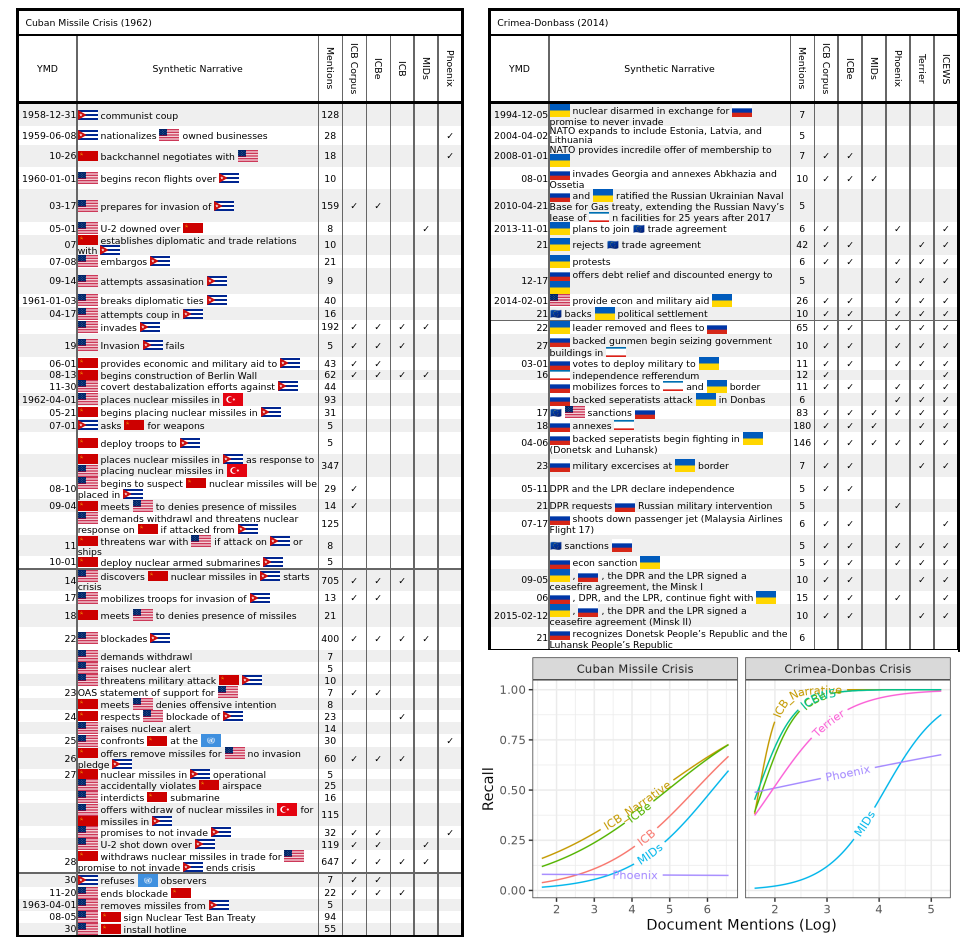
\includegraphics[height=18cm]{./recall_cuban_and_crimea_andcounts.png}}
\textit{Notes: Synthetic narratives combine several thousand accounts of each crisis into a single timeline of events, taking only those mentioned in at least 5 or more documents. Checkmarks represent whether that event could be hand matched to any detail in the ICB corpus, ICBe dataset, or any of the other event datasets (SI Appendix 3.2 and 3.3).}
\end{figure}
\clearpage

\hypertarget{precision}{%
\section{Precision}\label{precision}}

The other side of event measurement is precision, the degree to which a
sequence of events correctly and usefully describes the information in
history, \(Pr(H|E)\). It does little good to recall a historical event
but too vaguely (e.g.~MIDs describes the Cuban Missile Crisis as a
blockade, a show of force, and a stalemate) or with too much error
(e.g.~ICEWS records 263 ``Detonate Nuclear Weapons'' events between
1995-2019) to be useful for downstream applications. ICBe's ontology and
coding system are designed to strike a balance so that the most
important information is recovered accurately but also abstracted to a
level that is still useful and interpretable. You should be able to lay
out the events of a crisis on a timeline, as in Figure 3, and read off
the macrostructure of an episode from each individual move. We call this
visualization a crisis map, a directed graph intersected with a
timeline, and provide crisis maps for every event dataset for each case
study in SI Appendix 4.3 and 4.4 and for all crises on the companion
website.

We further want to verify individual event codings, which we can do in
the case of ICBe because each event is mapped to a specific span of
text. We develop the iconography system for presenting event codings as
coherent statements that can be compared side by side to the original
source narrative for Cuban Missiles (Figure 1), Crimea-Donbas (SI
Appendix 4.1), and for every case on the companion website. We further
provide a stratified sample of event codings alongside their source text
(SI Appendix 4.2).

We find both the visualizations of macrostructure and head-to-head
comparisons of ICBe codings to the raw text to strongly support the
quality of ICBe, but as with recall, we seek a more objective detached
universal benchmark. Our proposed measure is a reconstruction task to
see whether our intended ontology can be recovered through only
unsupervised clustering of sentences they were applied to. Figure 4
shows the location of every sentence from the ICBe corpus in semantic
space as embedded using the same large language model as before, and the
median location of each ICBe event tag applied to those
sentences.\footnote{We preprocess sentences to replace named entities
  with a generic Entity token.} Labels reflect the individual leaves of
the ontology and colors reflect the higher level coarse branch nodes of
the ontology. If ICBe has high precision, substantively similar tags
ought to have been applied to substantively similar source text, which
is what we see both in two dimensions in the main plot and via
hierarchical clustering on all dimensions in the dendrogram along the
righthand side.\footnote{Hierchcial clustering on cosine similarity and
  with Ward's method.}

Finally, how does ICBe's precision compare to the existing state of the
art? The crisis maps reveal the episode-level datasets like MIDs or the
original ICB are too sparse and vague to reconstruct the structure of
the crisis (SI Appendix 4.3 and 4.4). On the other end of the spectrum,
the high recall dictionary-based event datasets like Terrier and ICEWs
produce so many noisy events (several hundred thousand) that even with
heavy filtering their crisis maps are completely unintelligible.
Further, because of copyright issues, none of these datasets directly
provide the original text spans making event-level precision difficult
to verify.

However, given their high recall on our task and the global and
real-time coverage of dictionary-based event systems, we want to take
seriously the possibility that some functional transformation could
recover the precision of ICBe. For example, Terechshenko (2020) attempts
to correct for the mechanically increasing amount of news coverage each
year by detrending violent event counts from Phoenix using a human-coded
baseline. Others have focused on verifying precision for ICEWs on
specific subsets of details against known ground truths,
e.g.~geolocation (Cook and Weidmann 2019), protest events (80\%) (Wüest
and Lorenzini 2020), anti-government protest networks (46.1\%) (Jäger
2018).

We take the same approach here in Figure 5, selecting four specific
CAMEO event codings and checking how often they reflect a true
real-world event from the Crimea-Donbas synthetic narrative. We choose
four event types around key moments in the crisis. The start of the
crisis revolves around Ukraine backing out of a trade deal with the EU
in favor of Russia, but ``sign formal agreement'' events act more like a
topic detector with dozens of events generated by discussions of a
possible agreement but not the actual agreement which never
materialized. The switch is caught by the ``reject plan, agreement to
settle dispute'', but also continues for Victor Yanukovych even after he
was removed from power because of articles retroactively discussing the
cause of his removal. Events for ``use conventional military force''
capture a threshold around the start of hostilities and who the
participants were but not any particular battles or campaigns. Likewise,
``impose embargo, boycott, or sanctions'' captures the start of waves of
sanctions and from who but are effectively constant as the news coverage
does not distinguish between subtle changes or additions. In sum,
dictionary-based methods on news corpora tend to have high recall
because they parse everything in the news, but for the same reason,
their specificity for most event types is too low to back out individual
chess-like sequencing that ICBe aims to record.

\begin{figure}[H]
\caption{Crisis Map: Cuban Missile Crisis \label{fig:p_196_icbe}}
\centering{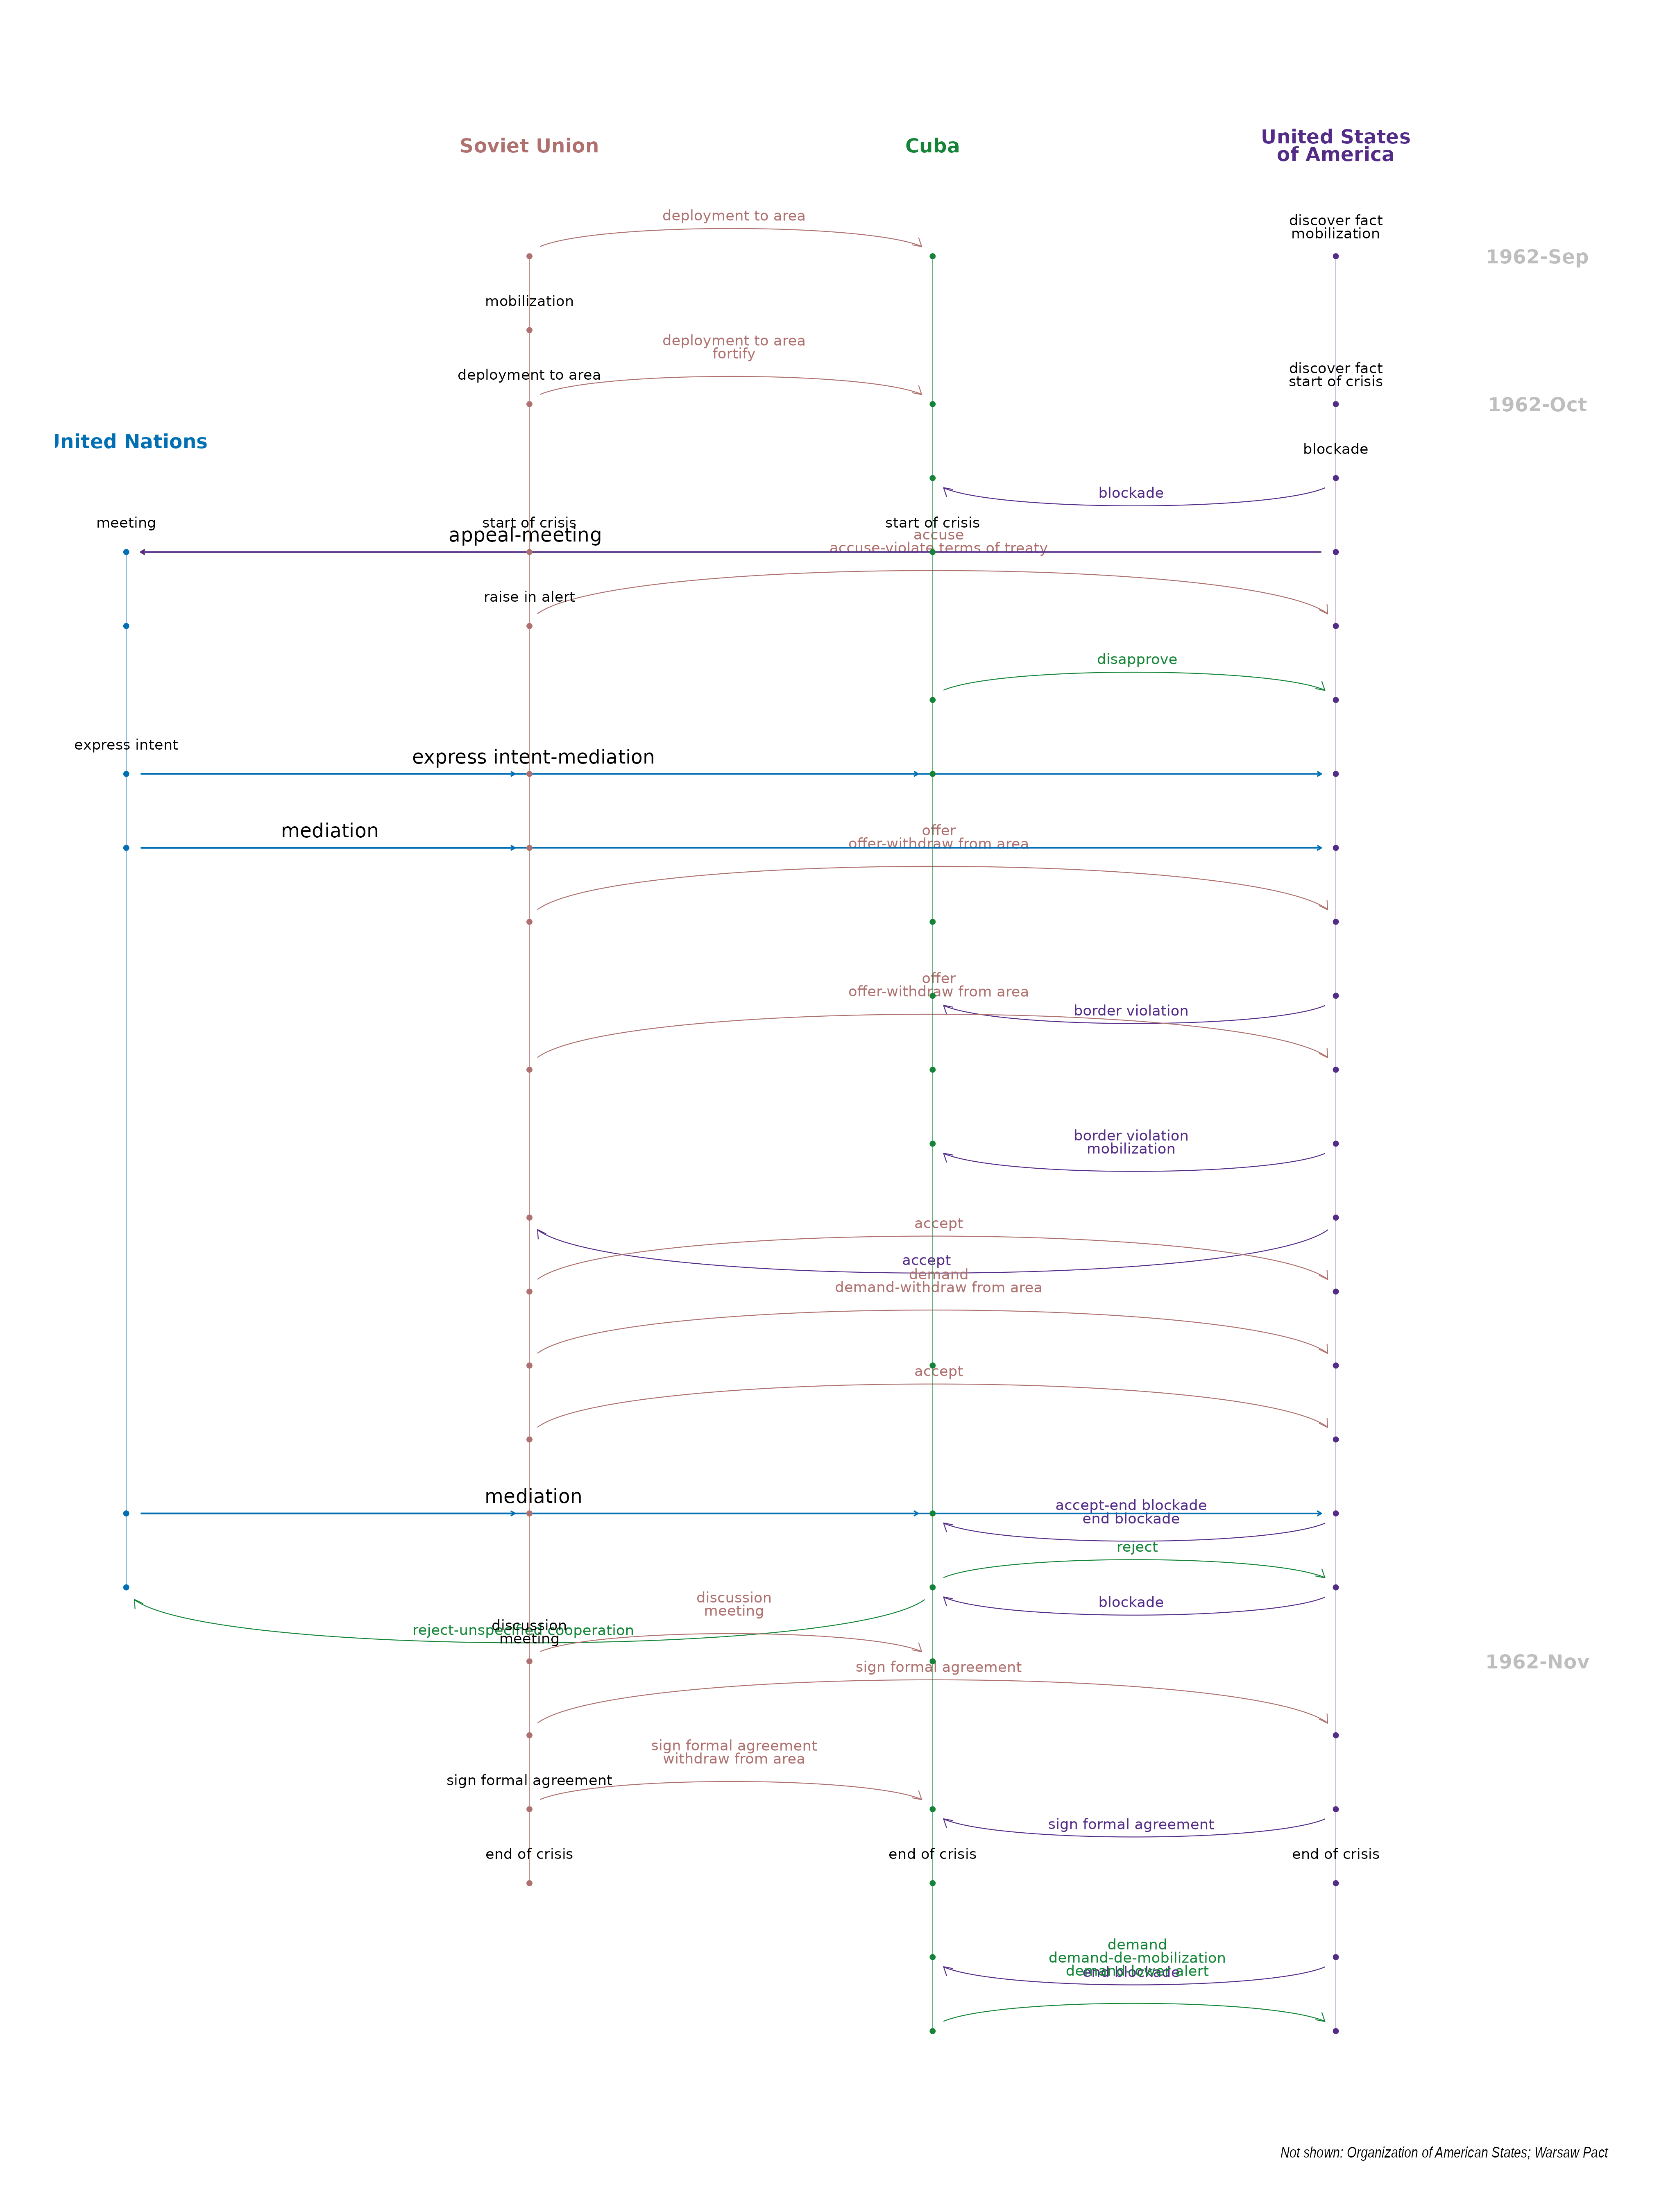
\includegraphics[width=16cm]{./p_196_icbe.png}}
\end{figure}

\clearpage

\begin{figure}[H]
\caption{ICBe event codings in comparison to Semantic Embeddings from source sentences\label{fig:semantic_embeddings}}
\centering{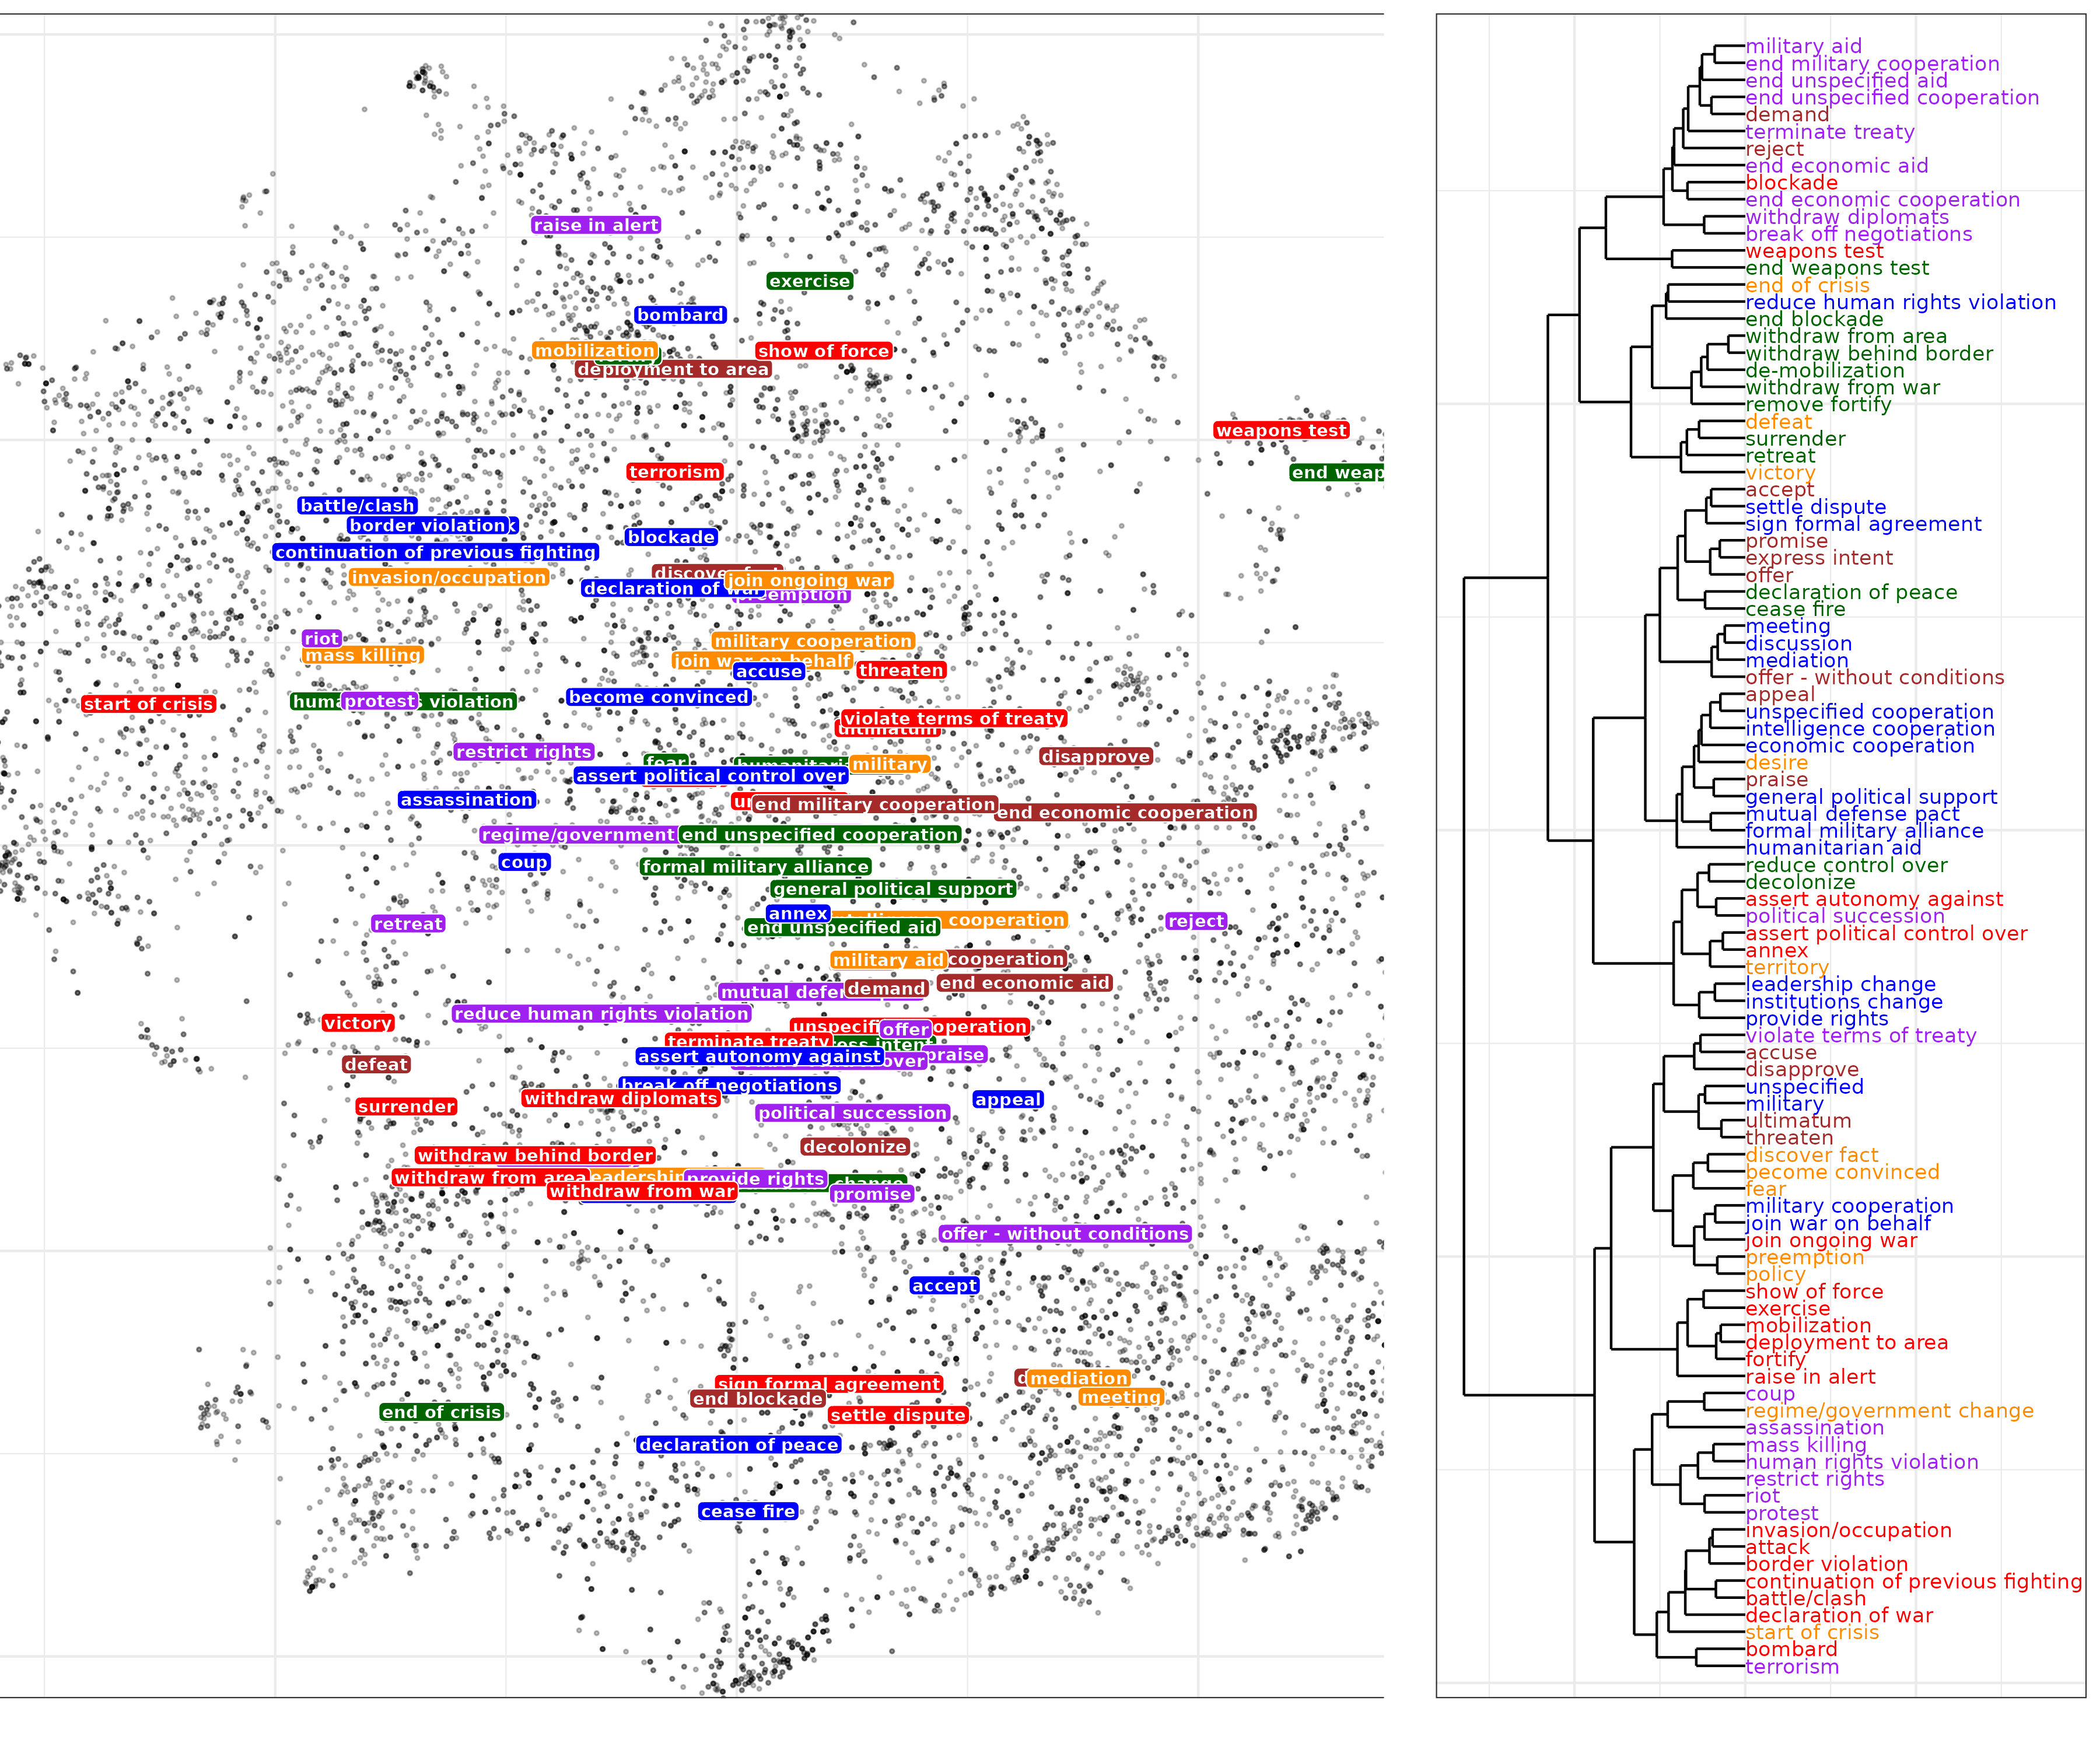
\includegraphics[width=17cm]{./p_semantic_embeddings_dendro.png}}
\textit{Notes: Dots represent individual ICB narrative sentences, as embedded by the Paraphrase-MPNET-base-v2 large language model and flattened into two dimensions with UMAP. Text labels reflect individual leaves of the ICBe ontology, and colors represent intermediate branches of the ontology. Label placement is the median of all of the sentences that the tag was applied to by the coders. The dendrogram shows hierarchical clustering of the tags. If ICBe precision is high, then the sentences that tags were applied to ought to say similar things and the intended shape of the ontology ought to be visually recognizable. }
\end{figure}
\clearpage

\clearpage

\begin{figure}[H]
\caption{ICEWs Events by Day by Type during the Crimea-Donbas Crisis \label{fig:p_precision_icews}}
\centering{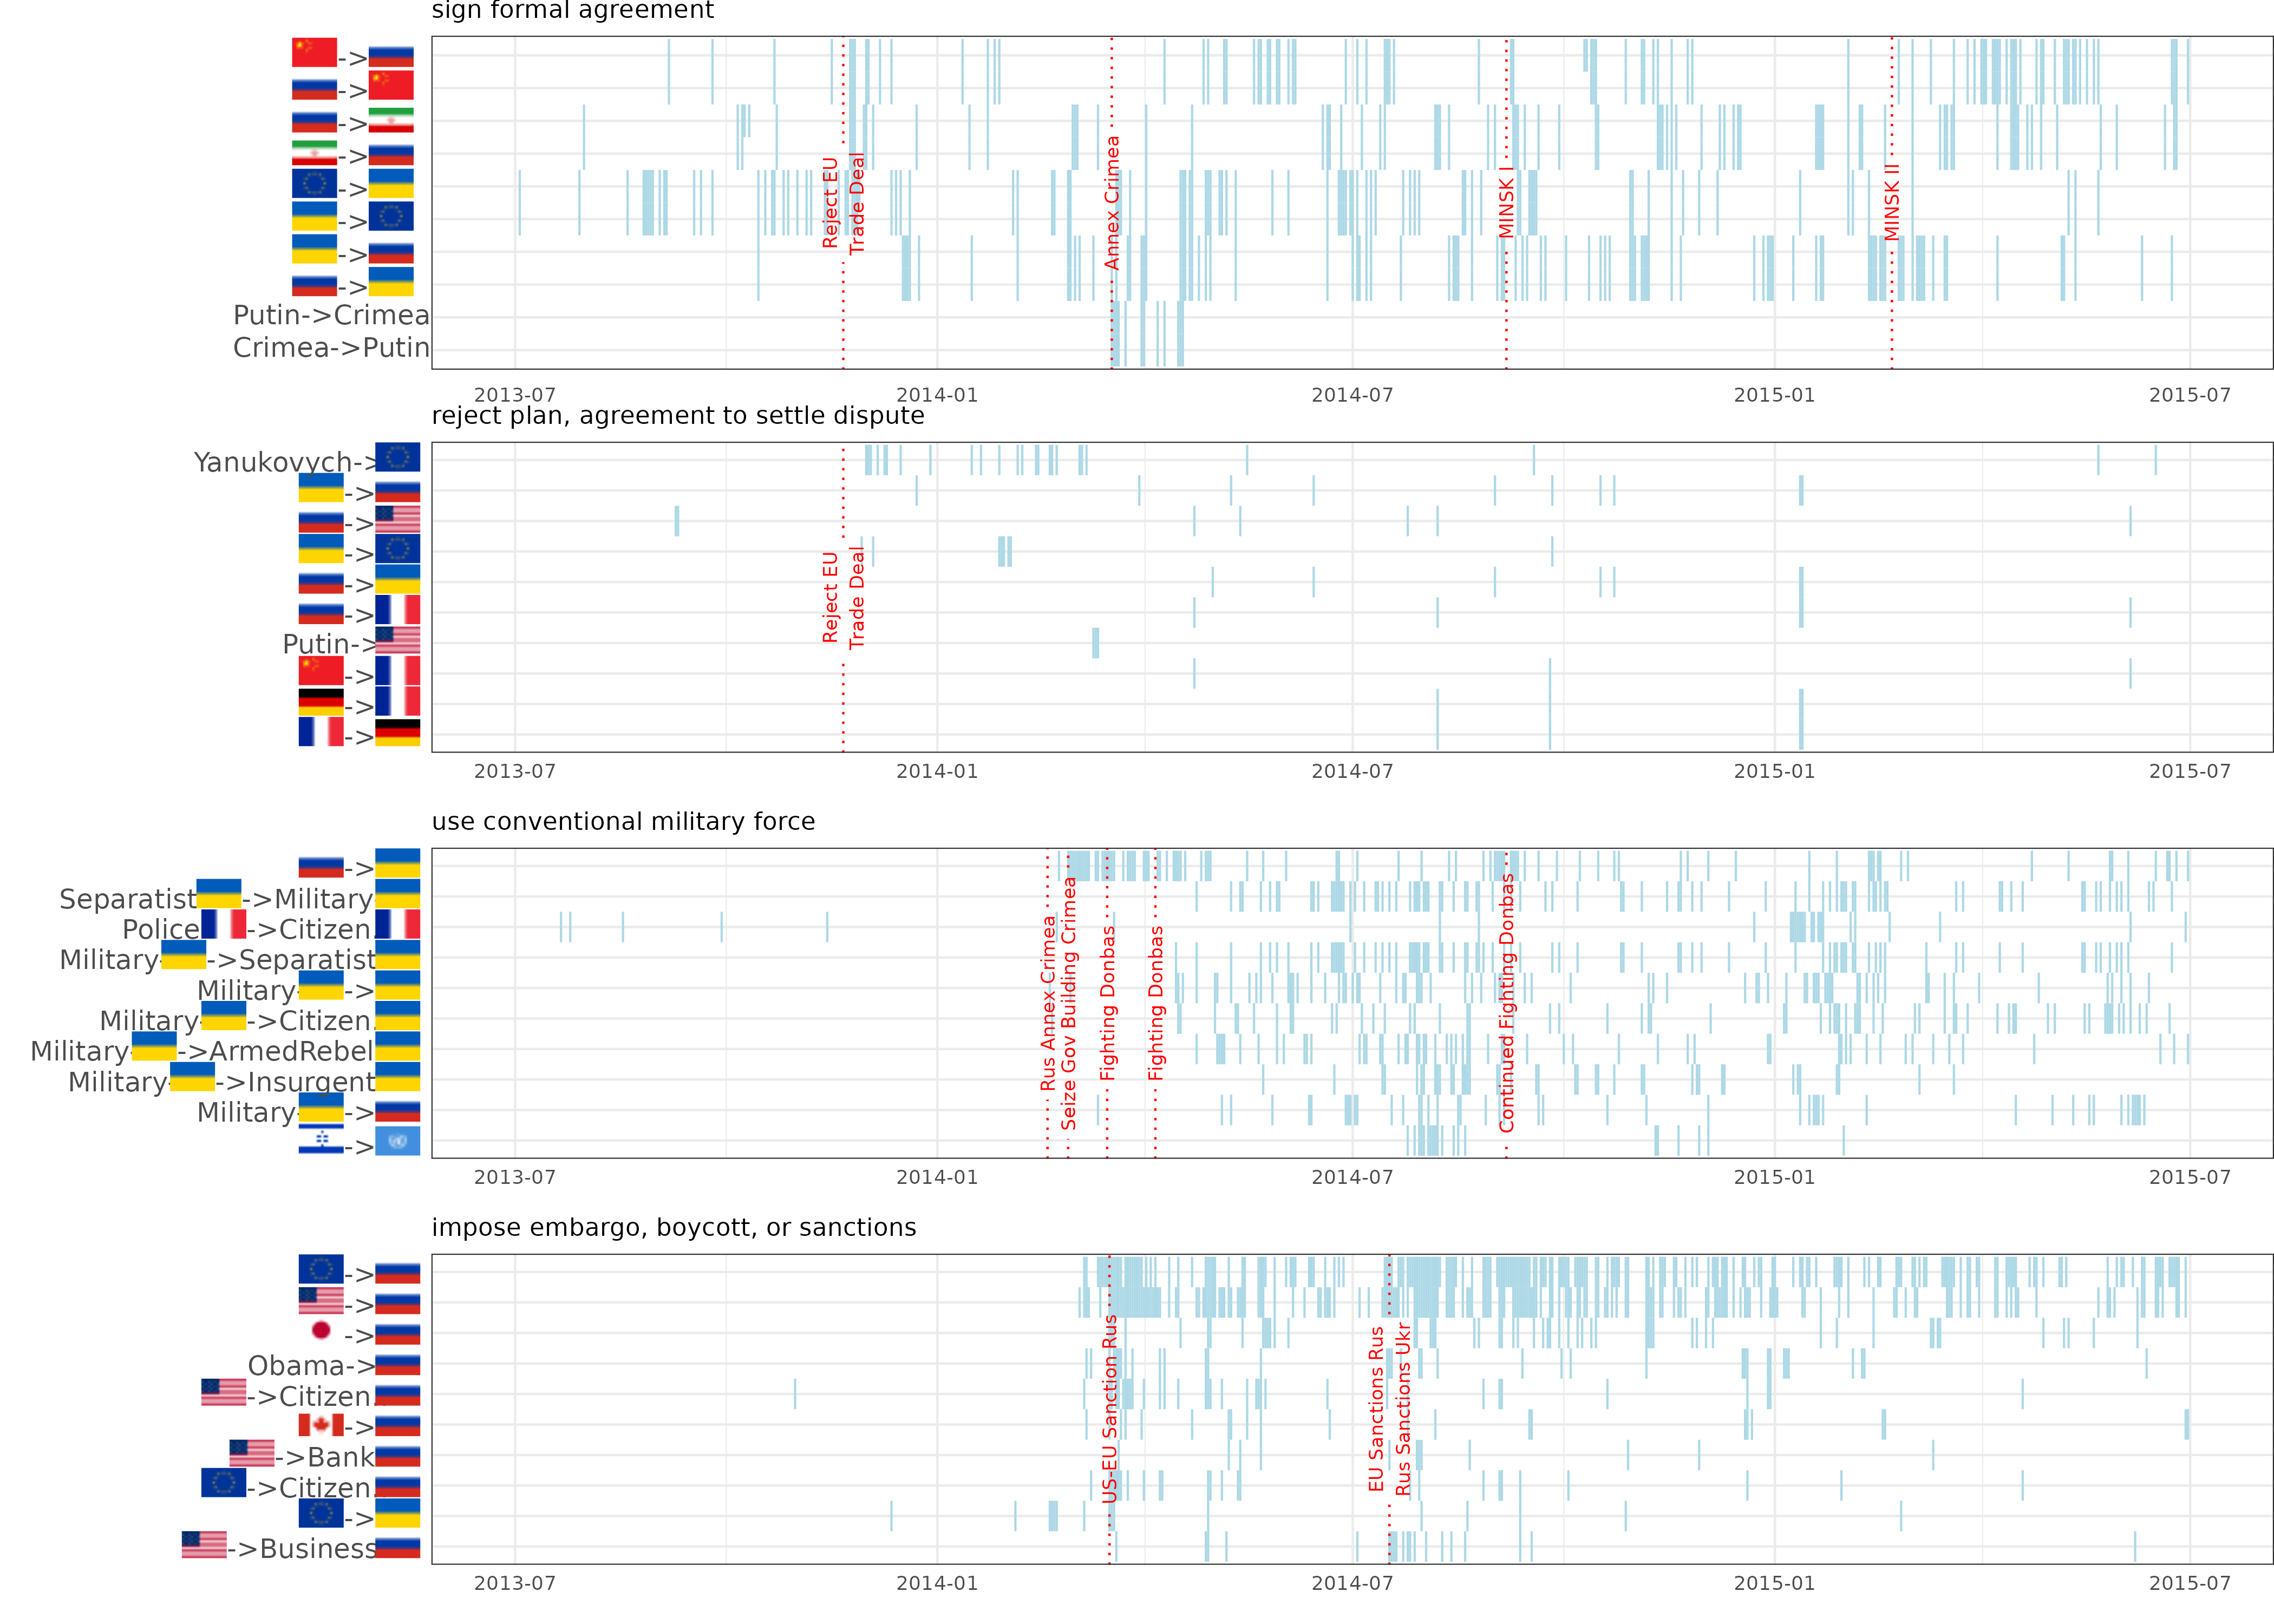
\includegraphics[width=17cm]{./p_precision_icews.png}}
\textit{Notes: The unit of analysis is the Dyad-Day. Top 10 most active dyads per category shown. Red text shows events from the synthetic narrative relative to that event category. Blue bars indicate an event recorded by ICEWs for that dyad on that day. }
\end{figure}
\clearpage

\hypertarget{conclusion}{%
\section{Conclusion}\label{conclusion}}

We investigated event abstraction from narratives describing key
historical episodes in international relations. We synthesized a prior
belief about the latent unobserved phenomena that drive these events in
international relations and proposed a mapping to observable concepts
that enter into the observed historical record. We designed an ontology
with high coverage over those concepts and developed a training
procedure and technical stack for human coding of historical texts.
Multiple validity checks find the resulting codings have high internal
validity (e.g.~intercoder agreement) and external validity
(i.e.~matching source material in both micro-details at the sentence
level and macro-details spanning full historical episodes). Further,
these codings perform much better in terms of recall, precision,
coverage, and overall coherence in capturing these historical episodes
than existing event systems used in international relations.

We release several open-source products along with supporting code and
documentation to further advance the study of IR, event extraction, and
natural language processing. The first is the International Crisis
Behavior Events (ICBe) dataset, an event-level aggregation of what took
place during the crises identified by the ICB project. These data are
appropriate for statistical analysis of hard questions about the
sequencing of events (e.g.~escalation and de-escalation of
conflicts).\footnote{Using ICBe data Gannon (2022) finds that
  cross-domain crises are shorter and less violent than same-domain
  crises.} Second, we provide a coder-level disaggregation with multiple
codings of each sentence by experts and undergrads that allows for the
introduction of uncertainty and human interpretation of events. Further,
we release a direct mapping from the codings to the source text at the
sentence level as a new resource for natural language processing.
Finally, we provide a companion website that incorporates detailed
visualizations of all of the data introduced here
(www.crisisevents.org).

\hypertarget{funding}{%
\section{Funding}\label{funding}}

This work was supported by a grant from the Office of Naval Research
{[}N00014-19-1-2491{]} and from the Charles Koch Foundation
{[}20180481{]}.

\hypertarget{acknowledgements}{%
\section{Acknowledgements}\label{acknowledgements}}

We thank the ICB Project and its directors and contributors for their
foundational work and their help with this effort. We make special
acknowledgment of Michael Brecher for helping found the ICB project in
1975, creating a resource that continues to spark new insights to this
day. We thank the many undergraduate coders for their patience and
dedication. Thanks to the Center for Peace and Security Studies and its
membership for comments. Special thanks to Rebecca Cordell, Philip
Schrodt, Zachary Steinert-Threlkeld, and Zhanna Terechshenko for their
generous feedback. Thank you to the cPASS research assistants that
contributed to this project: Helen Chung, Daman Heer, Syeda ShahBano
Ijaz, Anthony Limon, Erin Ling, Ari Michelson, Prithviraj Pahwa, Gianna
Pedro, Tobias Stodiek, Yiyi `Effie' Sun, Erin Werner, Lisa Yen, and
Ruixuan Zhang.

\hypertarget{author-contributions}{%
\section{Author Contributions}\label{author-contributions}}

Conceptualization: R.W.D., E.G., J.L.; Methodology: R.W.D., T.L.S.;
Software: R.W.D.; Validation: R.W.D., T.L.S.; Formal Analysis: R.W.D.,
T.L.S.; Investigation: S.C., R.W.D., J.A.G., C.K., N.L., E.M., J.M.C.N.,
D.P., D.Q., J.W.; Data Curation: R.W.D., D.Q., T.L.S., J.W.; Writing -
Original Draft: R.W.D., T.L.S.; Writing - Review \& Editing: R.W.D.,
J.A.G., E.G., T.L.S.; Visualization: R.W.D., T.L.S.; Supervision: E.G.;
Project Administration: S.C., R.W.D., J.A.G., D.Q., T.L.S., J.W.;
Funding Acquisition: E.G., J.L.

\hypertarget{data-availability-statement}{%
\section{Data Availability
Statement}\label{data-availability-statement}}

This article's data, supplementary appendix, replication material, and
visualizations of every historical episode are available on the GitHub
repository
\href{https://urldefense.com/v3/__https://github.com/CenterForPeaceAndSecurityStudies/ICBEventData__;!!Mih3wA!WxDJtEczKfxGTh0S2Krunap8ReymFEL5iTWaSfOHeqlSdyfRx77zmjBSWO1OAm13$}{ICBEventData}
and through the companion website www.crisisevents.org.

\hypertarget{conflicts-of-interests}{%
\section{Conflicts of Interests}\label{conflicts-of-interests}}

There are no conflicts of interest to disclose.

\clearpage

\hypertarget{works-cited}{%
\section*{Works Cited}\label{works-cited}}
\addcontentsline{toc}{section}{Works Cited}

\hypertarget{refs}{}
\begin{CSLReferences}{1}{0}
\leavevmode\vadjust pre{\hypertarget{ref-allenUSGlobalMilitary2021}{}}%
Allen, Michael A, Michael E Flynn, and Carla Martinez Machain. 2021.
{``{US} Global Military Deployments, 1950\textendash 2020*.''}
\emph{Conflict Management and Peace Science}, July, 07388942211030885.
\url{https://doi.org/10.1177/07388942211030885}.

\leavevmode\vadjust pre{\hypertarget{ref-allisonEssenceDecisionExplaining1971}{}}%
Allison, Graham T., and Philip Zelikow. 1971. \emph{Essence of Decision:
{Explaining} the {Cuban} Missile Crisis}. Vol. 327. {Little, Brown
Boston}.

\leavevmode\vadjust pre{\hypertarget{ref-althausClineCenterHistorical2019}{}}%
Althaus, Scott, Joseph Bajjalieh, John F. Carter, Buddy Peyton, and Dan
A. Shalmon. 2019. {``Cline {Center Historical Phoenix Event Data
Variable Descriptions}.''} \emph{Cline Center Historical Phoenix Event
Data}.

\leavevmode\vadjust pre{\hypertarget{ref-balaliCOfEEComprehensiveOntology2021}{}}%
Balali, Ali, Masoud Asadpour, and Seyed Hossein Jafari. 2021.
{``{COfEE}: {A Comprehensive Ontology} for {Event Extraction} from
Text.''} {arXiv}. \url{https://doi.org/10.48550/arXiv.2107.10326}.

\leavevmode\vadjust pre{\hypertarget{ref-barariDemocracyTradePolicy}{}}%
Barari, Soubhik, and In Song Kim. n.d. {``Democracy and {Trade Policy}
at the {Product Level}: {Evidence} from a {New Tariff-line Dataset},''}
16.

\leavevmode\vadjust pre{\hypertarget{ref-beardsleyMediationDilemma2011}{}}%
Beardsley, Kyle. 2011. \emph{The Mediation Dilemma}. {Cornell University
Press}.

\leavevmode\vadjust pre{\hypertarget{ref-beardsleyInternationalCrisisBehavior2020}{}}%
Beardsley, Kyle, Patrick James, Jonathan Wilkenfeld, and Michael
Brecher. 2020. {``The {International Crisis Behavior Project}.''}
\emph{Oxford Research Encyclopedia of Politics}.
https://oxfordre.com/politics/view/10.1093/acrefore/9780190228637.001.0001/acrefore-9780190228637-e-1638.
\url{https://doi.org/10.1093/acrefore/9780190228637.013.1638}.

\leavevmode\vadjust pre{\hypertarget{ref-benyehudaEthnicActorsInternational2006}{}}%
Ben-Yehuda, Hemda, and Meirav mishaliram. 2006. {``Ethnic {Actors} and
{International Crises}: {Theory} and {Findings},
1918\textendash 2001.''} \emph{International Interactions} 32 (1):
49--78. \url{https://doi.org/10.1080/03050620600584435}.

\leavevmode\vadjust pre{\hypertarget{ref-bloomfieldCASCONIIIComputeraided1989}{}}%
Bloomfield, Lincoln P., and Allen Moulton. 1989. {``{CASCON III}:
{Computer-aided} System for Analysis of Local Conflicts.''} \emph{MIT
Center for International Studies, Cambridge}.

\leavevmode\vadjust pre{\hypertarget{ref-boscheeICEWSCodedEvent2015}{}}%
Boschee, Elizabeth, Jennifer Lautenschlager, Sean O'Brien, Steve
Shellman, James Starz, and Michael Ward. 2015. {``{ICEWS} Coded Event
Data.''} \emph{Harvard Dataverse} 12.

\leavevmode\vadjust pre{\hypertarget{ref-braithwaiteCodebookMilitarizedInterstate2009}{}}%
Braithwaite, Alex. 2009. {``Codebook for the {Militarized Interstate
Dispute Location} ({MIDLOC}) {Data}, v 1.0.''} \emph{University College
London}.

\leavevmode\vadjust pre{\hypertarget{ref-braithwaiteMIDLOCIntroducingMilitarized2010}{}}%
---------. 2010. {``{MIDLOC}: {Introducing} the {Militarized Interstate
Dispute Location} Dataset.''} \emph{Journal of Peace Research} 47 (1):
91--98. \url{https://doi.org/10.1177/0022343309350008}.

\leavevmode\vadjust pre{\hypertarget{ref-brandtPhoenixRealTimeEvent2018}{}}%
Brandt, Patrick T., Vito DOrazio, Jennifer Holmes, Latifur Khan, and
Vincent Ng. 2018. {``Phoenix {Real-Time Event Data}.''}

\leavevmode\vadjust pre{\hypertarget{ref-brecherInternationalStudiesTwentieth1999}{}}%
Brecher, Michael. 1999. {``International Studies in the Twentieth
Century and Beyond: {Flawed} Dichotomies, Synthesis, Cumulation: {ISA}
Presidential Address.''} \emph{International Studies Quarterly} 43 (2):
213--64.

\leavevmode\vadjust pre{\hypertarget{ref-brecherPatternsCrisisManagement1988}{}}%
Brecher, Michael, and Patrick James. 1988. {``Patterns of Crisis
Management.''} \emph{Journal of Conflict Resolution} 32 (3): 426--56.

\leavevmode\vadjust pre{\hypertarget{ref-brecherCrisisEscalationWar2000}{}}%
Brecher, Michael, Patrick James, and Jonathan Wilkenfeld. 2000.
{``Crisis Escalation to War: {Findings} from the {International Crisis
Behavior Project}.''} \emph{What Do We Know About War}.

\leavevmode\vadjust pre{\hypertarget{ref-brecherCrisesWorldPolitics1982}{}}%
Brecher, Michael, and Jonathan Wilkenfeld. 1982. {``Crises in {World
Politics}.''} \emph{World Politics} 34 (3): 380--417.
\url{https://doi.org/10.2307/2010324}.

\leavevmode\vadjust pre{\hypertarget{ref-brecher_study_1997}{}}%
---------. 1997. \emph{A {Study} of {Crisis}}. {University of Michigan
Press}.

\leavevmode\vadjust pre{\hypertarget{ref-brecherInternationalCrisisBehavior2017}{}}%
Brecher, Michael, Jonathan Wilkenfeld, Kyle C. Beardsley, Patrick James,
and David Quinn. 2017. {``International {Crisis Behavior Data
Codebook}.''} Codebook Version 12.

\leavevmode\vadjust pre{\hypertarget{ref-brecherInternationalCrisisBehavior}{}}%
Brecher, Michael, Jonathan Wilkenfeld, Kyle Beardsley, Patrick James,
and David Quinn. n.d. {``International {Crisis Behavior Data Codebook},
{Version} 12,''} 69.

\leavevmode\vadjust pre{\hypertarget{ref-brustIntegratingDomainKnowledge2020}{}}%
Brust, Clemens-Alexander, and Joachim Denzler. 2020. {``Integrating
Domain Knowledge: Using Hierarchies to Improve Deep Classifiers.''}
\emph{arXiv:1811.07125 {[}Cs{]}}, January.
\url{https://arxiv.org/abs/1811.07125}.

\leavevmode\vadjust pre{\hypertarget{ref-buenodemesquitaDomesticExplanationsInternational2012}{}}%
Bueno de Mesquita, Bruce, and Alastair Smith. 2012. {``Domestic
{Explanations} of {International Relations}.''} \emph{Annual Review of
Political Science} 15 (1): 161--81.
\url{https://doi.org/10.1146/annurev-polisci-070209-174835}.

\leavevmode\vadjust pre{\hypertarget{ref-bushDensityDeclineFounding2019}{}}%
Bush, Sarah Sunn, and Jennifer Hadden. 2019. {``Density and {Decline} in
the {Founding} of {International NGOs} in the {United States}.''}
\emph{International Studies Quarterly} 63 (4): 1133--46.
\url{https://doi.org/10.1093/isq/sqz061}.

\leavevmode\vadjust pre{\hypertarget{ref-carafanoMeasuringMilitaryPower2014}{}}%
Carafano, James Jay. 2014. {``Measuring {Military Power}.''}
\emph{Strategic Studies Quarterly} 8 (3): 11--18.

\leavevmode\vadjust pre{\hypertarget{ref-carterStrategyTerritorialConflict2010}{}}%
Carter, David B. 2010. {``The {Strategy} of {Territorial Conflict}.''}
\emph{American Journal of Political Science} 54 (4): 969--87.
\url{https://doi.org/10.1111/j.1540-5907.2010.00471.x}.

\leavevmode\vadjust pre{\hypertarget{ref-chenowethIntroducingNonviolentAction2019}{}}%
Chenoweth, Erica, Cullen S Hendrix, and Kyleanne Hunter. 2019.
{``Introducing the {Nonviolent Action} in {Violent Contexts} ({NVAVC})
Dataset.''} \emph{Journal of Peace Research} 56 (2): 295--305.
\url{https://doi.org/10.1177/0022343318804855}.

\leavevmode\vadjust pre{\hypertarget{ref-cookLostAggregationImproving2019}{}}%
Cook, Scott J., and Nils B. Weidmann. 2019. {``Lost in {Aggregation}:
{Improving Event Analysis} with {Report-Level Data}.''} \emph{American
Journal of Political Science} 63 (1): 250--64.
\url{https://doi.org/10.1111/ajps.12398}.

\leavevmode\vadjust pre{\hypertarget{ref-cormacGreyNewBlack2018}{}}%
Cormac, Rory, and Richard J. Aldrich. 2018. {``Grey Is the New Black:
Covert Action and Implausible Deniability.''} \emph{International
Affairs} 94 (3): 477--94. \url{https://doi.org/10.1093/ia/iiy067}.

\leavevmode\vadjust pre{\hypertarget{ref-davisThreatsPromisesPursuit2000}{}}%
Davis, James W. 2000. \emph{Threats and {Promises}: {The Pursuit} of
{International Influence}}. {JHU Press}.

\leavevmode\vadjust pre{\hypertarget{ref-demesquitaForeignAidPolicy2007}{}}%
de Mesquita, Bruce Bueno, and Alastair Smith. 2007. {``Foreign {Aid} and
{Policy Concessions}.''} \emph{Journal of Conflict Resolution} 51 (2):
251--84. \url{https://doi.org/10.1177/0022002706297696}.

\leavevmode\vadjust pre{\hypertarget{ref-eckOneSidedViolenceCivilians2007}{}}%
Eck, Kristine, and Lisa Hultman. 2007. {``One-{Sided Violence Against
Civilians} in {War}: {Insights} from {New Fatality Data}.''}
\emph{Journal of Peace Research} 44 (2): 233--46.
\url{https://doi.org/10.1177/0022343307075124}.

\leavevmode\vadjust pre{\hypertarget{ref-fazalStateDeathPolitics2011}{}}%
Fazal, Tanisha M. 2011. \emph{State {Death}: {The Politics} and
{Geography} of {Conquest}, {Occupation}, and {Annexation}}. \emph{State
Death}. {Princeton University Press}.
\url{https://doi.org/10.1515/9781400841448}.

\leavevmode\vadjust pre{\hypertarget{ref-felbermayrGlobalSanctionsData2020}{}}%
Felbermayr, Gabriel, Aleksandra Kirilakha, Constantinos Syropoulos,
Erdal Yalcin, and Yoto V. Yotov. 2020. {``The Global Sanctions Data
Base.''} \emph{European Economic Review} 129 (October): 103561.
\url{https://doi.org/10.1016/j.euroecorev.2020.103561}.

\leavevmode\vadjust pre{\hypertarget{ref-fortnaPeaceTime2018}{}}%
Fortna, Virginia Page. 2018. \emph{Peace Time}. {Princeton University
Press}.

\leavevmode\vadjust pre{\hypertarget{ref-frederickIssueCorrelatesWar2017}{}}%
Frederick, Bryan A, Paul R Hensel, and Christopher Macaulay. 2017.
{``The {Issue Correlates} of {War Territorial Claims Data},
1816\textendash 20011.''} \emph{Journal of Peace Research} 54 (1):
99--108. \url{https://doi.org/10.1177/0022343316676311}.

\leavevmode\vadjust pre{\hypertarget{ref-gaddisExpandingDataBase1987}{}}%
Gaddis, John Lewis. 1987. {``Expanding the {Data Base}: {Historians},
{Political Scientists}, and the {Enrichment} of {Security Studies}.''}
\emph{International Security} 12 (1): 3--21.
\url{https://doi.org/10.2307/2538915}.

\leavevmode\vadjust pre{\hypertarget{ref-gannonOneIfLand2022}{}}%
Gannon, J Andrés. 2022. {``One If by {Land}, and {Two} If by {Sea}:
{Cross-Domain Contests} and the {Escalation} of {International
Crises}.''} \emph{International Studies Quarterly} 66 (4): sqac065.
\url{https://doi.org/10.1093/isq/sqac065}.

\leavevmode\vadjust pre{\hypertarget{ref-gartzkeCrossDomainDeterrenceStrategy2019}{}}%
Gartzke, Erik, and Jon R. Lindsay. 2019. \emph{Cross-{Domain
Deterrence}: {Strategy} in an {Era} of {Complexity}}. {Oxford University
Press}.

\leavevmode\vadjust pre{\hypertarget{ref-gavinHistorySecurityStudies2014}{}}%
Gavin, Francis J. 2014. {``History, {Security Studies}, and the {July
Crisis}.''} \emph{Journal of Strategic Studies} 37 (2): 319--31.
\url{https://doi.org/10.1080/01402390.2014.912916}.

\leavevmode\vadjust pre{\hypertarget{ref-georgeDeterrenceAmericanForeign1974}{}}%
George, Alexander L., and Richard Smoke. 1974. \emph{Deterrence in
{American} Foreign Policy: {Theory} and Practice}. {Columbia University
Press}.

\leavevmode\vadjust pre{\hypertarget{ref-giblerInternationalConflicts181620102018}{}}%
Gibler, Douglas M. 2018. \emph{International {Conflicts}, 1816-2010:
{Militarized Interstate Dispute Narratives}}. {Rowman \& Littlefield}.

\leavevmode\vadjust pre{\hypertarget{ref-giblerMeasuringAlliancesCorrelates2004}{}}%
Gibler, Douglas M., and Meredith Reid Sarkees. 2004. {``Measuring
{Alliances}: The {Correlates} of {War Formal Interstate Alliance}
{Dataset}, 1816\textendash 2000.''} \emph{Journal of Peace Research} 41
(2): 211--22. \url{https://doi.org/10.1177/0022343304041061}.

\leavevmode\vadjust pre{\hypertarget{ref-goemansIntroducingArchigosDataset2009}{}}%
Goemans, Henk E., Kristian Skrede Gleditsch, and Giacomo Chiozza. 2009.
{``Introducing {Archigos}: {A} Dataset of Political Leaders.''}
\emph{Journal of Peace Research} 46 (2): 269--83.

\leavevmode\vadjust pre{\hypertarget{ref-goertzMeasuringMilitaryAllocations1986}{}}%
Goertz, Gary, and Paul F. Diehl. 1986. {``Measuring {Military
Allocations}: {A Comparison} of {Different Approaches}.''} \emph{Journal
of Conflict Resolution} 30 (3): 553--81.
\url{https://doi.org/10.1177/0022002786030003009}.

\leavevmode\vadjust pre{\hypertarget{ref-goldgeierPsychologyInternationalRelations2001}{}}%
Goldgeier, J. M., and P. E. Tetlock. 2001. {``Psychology and
{International Relations Theory}.''} \emph{Annual Review of Political
Science} 4 (1): 67--92.
\url{https://doi.org/10.1146/annurev.polisci.4.1.67}.

\leavevmode\vadjust pre{\hypertarget{ref-grantOUEventData2017}{}}%
Grant, Christan, Andrew Halterman, Jill Irvine, Yan Liang, and Khaled
Jabr. 2017. {``{OU Event Data Project},''} December.

\leavevmode\vadjust pre{\hypertarget{ref-haffarEmergentPeacemakersCataloguing2002}{}}%
Haffar, Warren. 2002. {``Emergent {Peacemakers}: {Cataloguing New
Patterns} of {Activity} in {Post-Cold War Conflict}.''} \emph{Peace
Economics, Peace Science and Public Policy} 8 (2).
\url{https://doi.org/10.2202/1554-8597.1054}.

\leavevmode\vadjust pre{\hypertarget{ref-haltermanExtractingPoliticalEvents2020}{}}%
Halterman, Andy. 2020. {``Extracting {Political Events} from {Text Using
Syntax} and {Semantics}.''}

\leavevmode\vadjust pre{\hypertarget{ref-harknessEthnicArmyState2016}{}}%
Harkness, Kristen A. 2016. {``The Ethnic Army and the State:
{Explaining} Coup Traps and the Difficulties of Democratization in
{Africa}.''} \emph{Journal of Conflict Resolution} 60 (4): 587--616.

\leavevmode\vadjust pre{\hypertarget{ref-hegreIntroducingUCDPCandidate2020}{}}%
Hegre, Håvard, Mihai Croicu, Kristine Eck, and Stina Högbladh. 2020.
{``Introducing the {UCDP Candidate Events Dataset}.''} \emph{Research \&
Politics} 7 (3): 2053168020935257.

\leavevmode\vadjust pre{\hypertarget{ref-henselChartingCourseConflict1996}{}}%
Hensel, Paul R. 1996. {``Charting {A Course To Conflict}: {Territorial
Issues} and {Interstate Conflict}, 1816-1992.''} \emph{Conflict
Management and Peace Science} 15 (1): 43--73.
\url{https://doi.org/10.1177/073889429601500103}.

\leavevmode\vadjust pre{\hypertarget{ref-hermannComparativeResearchEvents1984}{}}%
Hermann, Charles. 1984. {``Comparative {Research} on the {Events} of
{Nations} ({CREON}) {Project}: {Foreign Policy Events}, 1959-1968:
{Version} 1.''} {ICPSR - Interuniversity Consortium for Political and
Social Research}. \url{https://doi.org/10.3886/ICPSR05205.V1}.

\leavevmode\vadjust pre{\hypertarget{ref-hewittEngagingInternationalData2001}{}}%
Hewitt, J. Joseph. 2001. {``Engaging {International Data} in the
{Classroom}: {Using} the {ICB Interactive Data Library} to {Teach
Conflict} and {Crisis Analysis}.''} \emph{International Studies
Perspectives} 2 (4): 371--83.
\url{https://doi.org/10.1111/1528-3577.00066}.

\leavevmode\vadjust pre{\hypertarget{ref-holsti1914Case1965}{}}%
Holsti, Ole R. 1965. {``The 1914 {Case}.''} \emph{The American Political
Science Review} 59 (2): 365--78. \url{https://doi.org/10.2307/1953055}.

\leavevmode\vadjust pre{\hypertarget{ref-iakhnisCrisesWorldPolitics2019}{}}%
Iakhnis, Evgeniia, and Patrick James. 2019. {``Near Crises in World
Politics: {A} New Dataset.''} \emph{Conflict Management and Peace
Science}, July, 0738894219855610.
\url{https://doi.org/10.1177/0738894219855610}.

\leavevmode\vadjust pre{\hypertarget{ref-jagerLimitsStudyingNetworks2018}{}}%
Jäger, Kai. 2018. {``The {Limits} of {Studying Networks} with {Event
Data}: {Evidence} from the {ICEWS Dataset}.''} \emph{Journal of Global
Security Studies} 3 (4): 498--511.

\leavevmode\vadjust pre{\hypertarget{ref-jamesWhatWeKnow2019}{}}%
James, Patrick. 2019. {``What Do We Know about Crisis, Escalation and
War? {A} Visual Assessment of the {International Crisis Behavior
Project}.''} \emph{Conflict Management and Peace Science} 36 (1): 3--19.
\url{https://doi.org/10.1177/0738894218793135}.

\leavevmode\vadjust pre{\hypertarget{ref-jonesHitMissEffect2009}{}}%
Jones, Benjamin F., and Benjamin A. Olken. 2009. {``Hit or {Miss}? {The
Effect} of {Assassinations} on {Institutions} and {War}.''}
\emph{American Economic Journal: Macroeconomics} 1 (2): 55--87.
\url{https://doi.org/10.1257/mac.1.2.55}.

\leavevmode\vadjust pre{\hypertarget{ref-kangUSBiasStudy2019}{}}%
Kang, David C., and Alex Yu-Ting Lin. 2019. {``{US} Bias in the Study of
{Asian} Security: {Using Europe} to Study {Asia}.''} \emph{Journal of
Global Security Studies} 4 (3): 393--401.

\leavevmode\vadjust pre{\hypertarget{ref-kinneDefenseCooperationAgreement2020}{}}%
Kinne, Brandon J. 2020. {``The {Defense Cooperation Agreement Dataset}
({DCAD}).''} \emph{Journal of Conflict Resolution} 64 (4): 729--55.
\url{https://doi.org/10.1177/0022002719857796}.

\leavevmode\vadjust pre{\hypertarget{ref-kuznetsovTheoryPracticeParadiplomacy2014}{}}%
Kuznetsov, Alexander. 2014. \emph{Theory and {Practice} of
{Paradiplomacy}: {Subnational Governments} in {International Affairs}}.
{London}: {Routledge}. \url{https://doi.org/10.4324/9781315817088}.

\leavevmode\vadjust pre{\hypertarget{ref-lacinaExplainingSeverityCivil2006}{}}%
Lacina, Bethany. 2006. {``Explaining the {Severity} of {Civil Wars}.''}
\emph{Journal of Conflict Resolution} 50 (2): 276--89.
\url{https://doi.org/10.1177/0022002705284828}.

\leavevmode\vadjust pre{\hypertarget{ref-lacinaMonitoringTrendsGlobal2005}{}}%
Lacina, Bethany, and Nils Petter Gleditsch. 2005. {``Monitoring {Trends}
in {Global Combat}: {A New Dataset} of {Battle Deaths}.''}
\emph{European Journal of Population / Revue Européenne de Démographie}
21 (2): 145--66. \url{https://doi.org/10.1007/s10680-005-6851-6}.

\leavevmode\vadjust pre{\hypertarget{ref-lafreeIntroducingGlobalTerrorism2007}{}}%
LaFree, Gary, and Laura Dugan. 2007. {``Introducing the Global Terrorism
Database.''} \emph{Terrorism and Political Violence} 19 (2): 181--204.

\leavevmode\vadjust pre{\hypertarget{ref-laiEffectsDifferentTypes2004}{}}%
Lai, Brian. 2004. {``The Effects of Different Types of Military
Mobilization on the Outcome of International Crises.''} \emph{Journal of
Conflict Resolution} 48 (2): 211--29.

\leavevmode\vadjust pre{\hypertarget{ref-lanoszkaLandpowerAmericanCredibility2016}{}}%
Lanoszka, Alexander, and Michael A. Hunzeker. 2016. {``Landpower and
{American} Credibility.''} \emph{Parameters: The United States Army's
Senior Professional Journal} 45 (4): 17--26.

\leavevmode\vadjust pre{\hypertarget{ref-leedsDomesticPoliticalInstitutions1999}{}}%
Leeds, Brett Ashley. 1999. {``Domestic {Political Institutions},
{Credible Commitments}, and {International Cooperation}.''}
\emph{American Journal of Political Science} 43 (4): 979--1002.
\url{https://doi.org/10.2307/2991814}.

\leavevmode\vadjust pre{\hypertarget{ref-leedsAllianceReliabilityTimes2003}{}}%
---------. 2003. {``Alliance {Reliability} in {Times} of {War}:
{Explaining State Decisions} to {Violate Treaties}.''}
\emph{International Organization} 57 (4): 801--27.
\url{https://doi.org/10.1017/S0020818303574057}.

\leavevmode\vadjust pre{\hypertarget{ref-lengMilitarizedInterstateCrises1988}{}}%
Leng, Russell J., and J. David Singer. 1988. {``Militarized {Interstate
Crises}: {The BCOW Typology} and {Its Applications}.''}
\emph{International Studies Quarterly} 32 (2): 155--73.
\url{https://doi.org/10.2307/2600625}.

\leavevmode\vadjust pre{\hypertarget{ref-levyCausesWar2011}{}}%
Levy, Jack S., and William R. Thompson. 2011. \emph{Causes of War}.
{John Wiley \& Sons}.

\leavevmode\vadjust pre{\hypertarget{ref-liComprehensiveSurveySchemabased2021}{}}%
Li, Qian, Hao Peng, Jianxin Li, Yiming Hei, Rui Sun, Jiawei Sheng, Shu
Guo, et al. 2021. {``A {Comprehensive Survey} on {Schema-based Event
Extraction} with {Deep Learning}.''} \emph{arXiv:2107.02126 {[}Cs{]}},
August. \url{https://arxiv.org/abs/2107.02126}.

\leavevmode\vadjust pre{\hypertarget{ref-lindsayPoliticsManyOther2020}{}}%
Lindsay, Jon R., and Erik Gartzke. 2020. {``Politics by Many Other
Means: {The} Comparative Strategic Advantages of Operational Domains.''}
\emph{Journal of Strategic Studies} 0 (0): 1--34.
\url{https://doi.org/10.1080/01402390.2020.1768372}.

\leavevmode\vadjust pre{\hypertarget{ref-luptonReexaminingReputationResolve2018}{}}%
Lupton, Danielle L. 2018. {``Reexamining {Reputation} for {Resolve}:
{Leaders}, {States}, and the {Onset} of {International Crises}.''}
\emph{Journal of Global Security Studies} 3 (2): 198--216.
\url{https://doi.org/10.1093/jogss/ogy004}.

\leavevmode\vadjust pre{\hypertarget{ref-mandelbrotFractalGeometryNature1983}{}}%
Mandelbrot, Benoit B. 1983. \emph{{The fractal geometry of nature}}.
{New York}: {Freeman}.

\leavevmode\vadjust pre{\hypertarget{ref-maozDyadicMilitarizedInterstate2019}{}}%
Maoz, Zeev, Paul L. Johnson, Jasper Kaplan, Fiona Ogunkoya, and Aaron P.
Shreve. 2019. {``The {Dyadic Militarized Interstate Disputes} ({MIDs})
{Dataset Version} 3.0: {Logic}, {Characteristics}, and {Comparisons} to
{Alternative Datasets}.''} \emph{Journal of Conflict Resolution} 63 (3):
811--35. \url{https://doi.org/10.1177/0022002718784158}.

\leavevmode\vadjust pre{\hypertarget{ref-matanockElectingPeaceCivil2017}{}}%
Matanock, Aila M. 2017. \emph{Electing {Peace}: {From Civil Conflict} to
{Political Participation}}. {Cambridge}: {Cambridge University Press}.
\url{https://doi.org/10.1017/9781316987179}.

\leavevmode\vadjust pre{\hypertarget{ref-mcclearyPrivateVoluntaryOrganizations2008}{}}%
McCleary, Rachel M., and Robert J. Barro. 2008. {``Private {Voluntary
Organizations Engaged} in {International Assistance}, 1939-2004.''}
\emph{Nonprofit and Voluntary Sector Quarterly} 37 (3): 512--36.
\url{https://doi.org/10.1177/0899764007313719}.

\leavevmode\vadjust pre{\hypertarget{ref-mcclellandWorldEventInteraction1978}{}}%
McClelland, Charles. 1978. {``World Event/Interaction Survey,
1966-1978.''} \emph{WEIS Codebook ICPSR} 5211.

\leavevmode\vadjust pre{\hypertarget{ref-mcnabbcochranMeasuringMilitaryEffectiveness2017}{}}%
McNabb Cochran, Kathryn, and Stephen B. Long. 2017. {``Measuring
{Military Effectiveness}: {Calculating Casualty Loss-Exchange Ratios}
for {Multilateral Wars}, 1816\textendash 1990.''} \emph{International
Interactions} 43 (6): 1019--40.
\url{https://doi.org/10.1080/03050629.2017.1273914}.

\leavevmode\vadjust pre{\hypertarget{ref-mercerProspectTheoryPolitical2005}{}}%
Mercer, Jonathan. 2005. {``Prospect {Theory} and {Political Science}.''}
\emph{Annual Review of Political Science} 8 (1): 1--21.
\url{https://doi.org/10.1146/annurev.polisci.8.082103.104911}.

\leavevmode\vadjust pre{\hypertarget{ref-merrittMeasuringEventsInternational1994}{}}%
Merritt, Richard L. 1994. {``Measuring Events for International
Political Analysis.''} \emph{International Interactions} 20 (1-2):
3--33.

\leavevmode\vadjust pre{\hypertarget{ref-millerWordNetLexicalDatabase1995}{}}%
Miller, George A. 1995. {``{WordNet}: A Lexical Database for
{English}.''} \emph{Communications of the ACM} 38 (11): 39--41.
\url{https://doi.org/10.1145/219717.219748}.

\leavevmode\vadjust pre{\hypertarget{ref-minInterstateWarBattle2021}{}}%
Min, Eric. 2021. {``Interstate {War Battle} Dataset
(1823\textendash 2003).''} \emph{Journal of Peace Research} 58 (2):
294--303. \url{https://doi.org/10.1177/0022343320913305}.

\leavevmode\vadjust pre{\hypertarget{ref-moyerWhatAreDrivers2020}{}}%
Moyer, Jonathan D, Sara D Turner, and Collin J Meisel. 2020. {``What Are
the Drivers of Diplomacy? {Introducing} and Testing New Annual Dyadic
Data Measuring Diplomatic Exchange.''} \emph{Journal of Peace Research},
September, 0022343320929740.
\url{https://doi.org/10.1177/0022343320929740}.

\leavevmode\vadjust pre{\hypertarget{ref-oneillInternationalNegotiationConceptual2018}{}}%
O'Neill, Barry. 2018. {``International {Negotiation}: {Some Conceptual
Developments}.''} \emph{Annual Review of Political Science} 21 (1):
515--33. \url{https://doi.org/10.1146/annurev-polisci-031416-092909}.

\leavevmode\vadjust pre{\hypertarget{ref-olterIntergovernmentalOrganizationsIGOs2021}{}}%
Olter, Agnieszka. 2021. {``Intergovernmental Organizations ({IGOs}) as
Relevant Actors in {International Relations}.''} \emph{Repositorio
Institucional - Ulima}.

\leavevmode\vadjust pre{\hypertarget{ref-owsiakInternationalBorderAgreements2018}{}}%
Owsiak, Andrew P, Allison K Cuttner, and Brent Buck. 2018. {``The
{International Border Agreements Dataset}.''} \emph{Conflict Management
and Peace Science} 35 (5): 559--76.
\url{https://doi.org/10.1177/0738894216646978}.

\leavevmode\vadjust pre{\hypertarget{ref-paigeKoreanDecisionJune1968}{}}%
Paige, Glenn D. 1968. \emph{The {Korean Decision}, {June} 24-30, 1950}.
{Free Press}.

\leavevmode\vadjust pre{\hypertarget{ref-palmerMID5Dataset20112021}{}}%
Palmer, Glenn, Roseanne W McManus, Vito D'Orazio, Michael R Kenwick,
Mikaela Karstens, Chase Bloch, Nick Dietrich, Kayla Kahn, Kellan Ritter,
and Michael J Soules. 2021. {``The {Mid5 Dataset}, 2011\textendash 2014:
{Procedures}, Coding Rules, and Description.''} \emph{Conflict
Management and Peace Science}, February, 0738894221995743.
\url{https://doi.org/10.1177/0738894221995743}.

\leavevmode\vadjust pre{\hypertarget{ref-petterssonOrganizedViolence19892018}{}}%
Pettersson, Therése, and Kristine Eck. 2018. {``Organized Violence,
1989\textendash 2017.''} \emph{Journal of Peace Research} 55 (4):
535--47. \url{https://doi.org/10.1177/0022343318784101}.

\leavevmode\vadjust pre{\hypertarget{ref-powellGlobalInstancesCoups2011}{}}%
Powell, Jonathan M, and Clayton L Thyne. 2011. {``Global Instances of
Coups from 1950 to 2010: {A} New Dataset.''} \emph{Journal of Peace
Research} 48 (2): 249--59.
\url{https://doi.org/10.1177/0022343310397436}.

\leavevmode\vadjust pre{\hypertarget{ref-powellBargainingTheoryInternational2002}{}}%
Powell, Robert. 2002. {``Bargaining {Theory} and {International
Conflict}.''} \emph{Annual Review of Political Science} 5 (1): 1--30.
\url{https://doi.org/10.1146/annurev.polisci.5.092601.141138}.

\leavevmode\vadjust pre{\hypertarget{ref-raleighIntroducingACLEDArmed2010}{}}%
Raleigh, Clionadh, Andrew Linke, Håavard Hegre, and Joakim Karlsen.
2010. {``Introducing {ACLED}: An Armed Conflict Location and Event
Dataset: Special Data Feature.''} \emph{Journal of Peace Research} 47
(5): 651--60.

\leavevmode\vadjust pre{\hypertarget{ref-ralphsundbergUCDPGEDCodebook2016}{}}%
Ralph Sundberg, and Mihai Croicu. 2016. {``{UCDP GED Codebook} Version
5.0.''} {Department of Peace and Conflict Research, Uppsala University}.

\leavevmode\vadjust pre{\hypertarget{ref-ramsayInformationUncertaintyWar2017}{}}%
Ramsay, Kristopher W. 2017. {``Information, {Uncertainty}, and {War}.''}
\emph{Annual Review of Political Science} 20 (1): 505--27.
\url{https://doi.org/10.1146/annurev-polisci-051215-022729}.

\leavevmode\vadjust pre{\hypertarget{ref-reiterHowWarsEnd2009}{}}%
Reiter, Dan. 2009. \emph{How Wars End}. {Princeton University Press}.

\leavevmode\vadjust pre{\hypertarget{ref-reiterShouldWeLeave2015}{}}%
---------. 2015. {``Should {We Leave Behind} the {Subfield} of
{International Relations}?''} \emph{Annual Review of Political Science}
18 (1): 481--99.
\url{https://doi.org/10.1146/annurev-polisci-053013-041156}.

\leavevmode\vadjust pre{\hypertarget{ref-reiterRevisedLookInterstate2016}{}}%
Reiter, Dan, Allan C. Stam, and Michael C. Horowitz. 2016. {``A {Revised
Look} at {Interstate Wars}, 1816\textendash 2007.''} \emph{Journal of
Conflict Resolution} 60 (5): 956--76.
\url{https://doi.org/10.1177/0022002714553107}.

\leavevmode\vadjust pre{\hypertarget{ref-ryanNationStatesEmpiresWars2021}{}}%
Ryan, Cheyney. 2021. {``Nation-{States}, {Empires}, {Wars},
{Hostilities}.''} \emph{Ethics \& International Affairs} 35 (3):
367--79.

\leavevmode\vadjust pre{\hypertarget{ref-sarkeesResortWar181620072010}{}}%
Sarkees, Meredith Reid, and Frank Wayman. 2010. \emph{Resort to War:
1816-2007}. {CQ Press}.

\leavevmode\vadjust pre{\hypertarget{ref-schrodtTwentyYearsKansas2006}{}}%
Schrodt, Philip A., and Blake Hall. 2006. {``Twenty Years of the
{Kansas} Event Data System Project.''} \emph{The Political
Methodologist} 14 (1): 2--8.

\leavevmode\vadjust pre{\hypertarget{ref-sechserMilitarizedCompellentThreats2011}{}}%
Sechser, Todd S. 2011. {``Militarized {Compellent Threats},
1918\textendash 2001.''} \emph{Conflict Management and Peace Science} 28
(4): 377--401. \url{https://doi.org/10.1177/0738894211413066}.

\leavevmode\vadjust pre{\hypertarget{ref-shermanSHERFACSCrossParadigmHierarchical2000}{}}%
Sherman, Frank L. 2000. {``{SHERFACS}: {A Cross-Paradigm},
{Hierarchical}, and {Contextually-Sensitive International Conflict
Dataset}, 1937-1985: {Version} 1.''} {ICPSR - Interuniversity Consortium
for Political and Social Research}.
\url{https://doi.org/10.3886/ICPSR02292.V1}.

\leavevmode\vadjust pre{\hypertarget{ref-snyderConflictNationsBargaining1977}{}}%
Snyder, Glenn Herald, and Paul Diesing. 1977. \emph{Conflict Among
Nations: {Bargaining} and Decision Making in International Crises}.
{Princeton University Press}.

\leavevmode\vadjust pre{\hypertarget{ref-spruytSovereignStateIts1996}{}}%
Spruyt, Hendrik. 1996. \emph{The {Sovereign State} and {Its
Competitors}: {An Analysis} of {Systems Change}}. {Princeton University
Press}.

\leavevmode\vadjust pre{\hypertarget{ref-steinEvaluatingWarOutcomes1980}{}}%
Stein, Arthur A., and Bruce M. Russett. 1980. {``Evaluating War:
{Outcomes} and Consequences.''} In \emph{Handbook of Political Conflict:
Theory and Research}, 399--422. {Free Press New York}.

\leavevmode\vadjust pre{\hypertarget{ref-steinert-threlkeldFutureEventData2019}{}}%
Steinert-Threlkeld, Zachary C. 2019. {``The {Future} of {Event Data Is
Images}.''} \emph{Sociological Methodology} 49 (1): 68--75.
\url{https://doi.org/10.1177/0081175019860238}.

\leavevmode\vadjust pre{\hypertarget{ref-sullivanWarAimsWar2007}{}}%
Sullivan, Patricia L. 2007. {``War {Aims} and {War Outcomes}: {Why
Powerful States Lose Limited Wars}.''} \emph{Journal of Conflict
Resolution} 51 (3): 496--524.
\url{https://doi.org/10.1177/0022002707300187}.

\leavevmode\vadjust pre{\hypertarget{ref-sundbergIntroducingUCDPGeoreferenced2013}{}}%
Sundberg, Ralph, and Erik Melander. 2013. {``Introducing the {UCDP}
Georeferenced Event Dataset.''} \emph{Journal of Peace Research} 50 (4):
523--32.

\leavevmode\vadjust pre{\hypertarget{ref-terechshenkoHotCollarLatent2020}{}}%
Terechshenko, Zhanna. 2020. {``Hot Under the Collar: {A} Latent Measure
of Interstate Hostility.''} \emph{Journal of Peace Research} 57 (6):
764--76. \url{https://doi.org/10.1177/0022343320962546}.

\leavevmode\vadjust pre{\hypertarget{ref-tragerDiplomacyWarPeace2016}{}}%
Trager, Robert F. 2016. {``The {Diplomacy} of {War} and {Peace}.''}
\emph{Annual Review of Political Science} 19 (1): 205--28.
\url{https://doi.org/10.1146/annurev-polisci-051214-100534}.

\leavevmode\vadjust pre{\hypertarget{ref-vabulasCooperationAutonomyBuilding2021}{}}%
Vabulas, Felicity, and Duncan Snidal. 2021. {``Cooperation Under
Autonomy: {Building} and Analyzing the {Informal Intergovernmental
Organizations} 2.0 Dataset.''} \emph{Journal of Peace Research} 58 (4):
859--69. \url{https://doi.org/10.1177/0022343320943920}.

\leavevmode\vadjust pre{\hypertarget{ref-wilkenfeldInterstateCrisesViolence2000}{}}%
Wilkenfeld, Jonathan, and Michael Brecher. 2000. {``Interstate Crises
and Violence: Twentieth-Century Findings.''} \emph{Handbook of War
Studies II}, 282--300.

\leavevmode\vadjust pre{\hypertarget{ref-wuestExternalValidationProtest2020}{}}%
Wüest, Bruno, and Jasmine Lorenzini. 2020. {``External Validation of
Protest Event Analysis.''} \emph{Contention in Times of Crisis:
Recession and Political Protest in Thirty Euro-Pean Countries}, 49--78.

\leavevmode\vadjust pre{\hypertarget{ref-yarhi-miloEyeBeholderHow2013}{}}%
Yarhi-Milo, Keren. 2013. {``In the {Eye} of the {Beholder}: {How
Leaders} and {Intelligence Communities Assess} the {Intentions} of
{Adversaries}.''} \emph{International Security} 38 (1): 7--51.
\url{https://doi.org/10.1162/ISEC_a_00128}.

\leavevmode\vadjust pre{\hypertarget{ref-yarhi-miloArmAllyPatron2016}{}}%
Yarhi-Milo, Keren, Alexander Lanoszka, and Zack Cooper. 2016. {``To
{Arm} or to {Ally}? {The Patron}'s {Dilemma} and the {Strategic Logic}
of {Arms Transfers} and {Alliances}.''} \emph{International Security} 41
(2): 90--139. \url{https://doi.org/10.1162/ISEC_a_00250}.

\leavevmode\vadjust pre{\hypertarget{ref-zartmanEscalationNegotiationInternational2005}{}}%
Zartman, I. William, and Guy Olivier Faure. 2005. \emph{Escalation and
Negotiation in International Conflicts}. {Cambridge University Press}.

\leavevmode\vadjust pre{\hypertarget{ref-zhangCASMDeepLearningApproach2019}{}}%
Zhang, Han, and Jennifer Pan. 2019. {``{CASM}: {A Deep-Learning
Approach} for {Identifying Collective Action Events} with {Text} and
{Image Data} from {Social Media}.''} \emph{Sociological Methodology} 49
(1): 1--57. \url{https://doi.org/10.1177/0081175019860244}.

\end{CSLReferences}

\bibliographystyle{unsrt}
\bibliography{paper.bib}


\end{document}
